\documentclass[12pt]{niuthesis}
% \documentclass[12pt,singlespacing]{niuthesis}

% some packages are loaded here

\usepackage{latexsym}		% to get LASY symbols
\usepackage{graphicx}		% to insert PostScript figures
\usepackage{rotating}           % defines sidways table and figure env.
% default env and hepunits has issues with degree - workaround 
\usepackage{savesym}
\savesymbol{degree}
\usepackage{hepunits}
\usepackage[hidelinks]{hyperref}
\usepackage[acronym]{glossaries}
\usepackage[style=numeric-comp,sorting=none,block=ragged,firstinits=true]{biblatex}
\renewbibmacro{in:}{}
\bibliography{biblio}

\usepackage{xcolor}
\usepackage{microtype}

\let\degree\relax
\restoresymbol{DEFAULT}{degree} % make sure this is ok
% \usepackage{hyperref}		% to insert hyperrefs

%%%%%%%%%%%%%%%%%%%%%%%%%%%%%%%%%%%%%%%%%%%%%%%%%%%%%%%%%%%%%%%%
% Some LaTeX macros

\newcommand{\twochoices}[2]{\left\{ \begin{array}{lcc}
        \displaystyle #1 \\ \vspace{-10pt} \\
        \displaystyle #2 \end{array} \right. } %}

\newcommand{\twovec}[2]{\left(\begin{array}{c} #1 \\ #2 \end{array}\right)}

\newcommand{\twomatrix}[4]{\left(\begin{array}{cc} #1 & #2 \\ 
     #3 & #4 \end{array}\right)}

% Uncomment the following line for a List of Symbols
% \newcommand{\listofXXX}{\input{symbols}}

%%%%%%%%%%%%%%%%%%%%%%%%%%%%%%%%%%%%%%%%%%%%%%%%%%%%%%%%%%%%%%%%%%
% Choose the chapter(s) / files you want to work with

%%% use this to compile all chapters
%\def\files{ch1,ch2,refs,app1,app2}

%%% use this to work with only one chapter
%\def\files{chapters/chapter2_experiment/experiment}

%\includeonly{\files}

%%%%%%%%%%%%%%%%%%%%%%%%%%%%%%%%%%%%%%%%%%%%%%%%%%%%%%%%%%%%%%%%%
\loadglsentries{glossary}
\makeglossaries
\begin{document}

\title{A search for resonant and non-resonant di-Higgs production in the $\gamma \gamma \lowercase{b \bar{b}}$ channel using the  ATLAS Detector}

\author{Tyler James Burch}

\major{Physics}
\degree{Dissertation}{Ph.D.}{Doctor of Philosophy}
\degreedate{December}{2019}
\department{Department of Physics}
\director{Jahred Adelman}


\begin{abstract}
  %short

%long

This dissertation uses 139 \ifb of \pp collision data collected at a center of mass energy of \sqs by the ATLAS detector to search for charged Higgs bosons decaying to a tau lepton and a neutrino (\HpLong) in association with a leptonically decaying top quark. No significant excess was found, therefore limits are set at the 95\% confidence level on the charged Higgs production cross section times the branching fraction into the \taunu ranging from XX pb to XX fb. These limits are interpreted in the hMSSM benchmark scenario as an exclusion at 95\% confidence on \tanb as a function of \mHp. In this scenario, for $\tanb=60$, the \Hp mass range up to $\unit{XXXX}{GeV}$ is excluded, with all values of \tanb excluded for $\mHp \leq \unit{XXX}{GeV}$
\end{abstract}

\begin{acknowledgments}

\end{acknowledgments}

\begin{dedication}

\end{dedication}

% comment this to suppress prologue
\MakeThesisPrologue % includes table of contents
\tableofcontents

\chapter{Theory}
    In this chapter, the theoretical motivation of a search for \HpLong is described. Firstly, a review of the Standard Model of particle physics (SM) is laid out, then a brief overview of Supersymmetry focusing on the Minimal Supersymmetric Standard Model (MSSM) Higgs sector is detailed. Finally, the Type II 2-Higgs Doublet Model's (2HDM) relation to the \Hp production cross section and subsequent branching ratio into SM particles is described as motivation for the choice of studying \HpLong.

\section{The Standard Model}
	The Standard Model of particle physics is a mathematical model that describes all known matter and forces. The Standard Model is built upon a gauge group of type $SU(3)_C \times SU(2)_L \times U(1)_Y$. The $SU(3)_C$ term dictates the strong interaction while the $SU(2)_L \times U(1)_Y$ term describes the electroweak interaction. These interactions occur between fundamental particles called fermions that comprise the known matter of the universe. The interactions, or forces, are mediated by fundamental particles called bosons. 

	\subsection{Particles}        
		The particles that make up the Standard Model are separated into two groups according to their intrinsic angular momentum charge, or spin. Fermions are those that carry half-integer spin while Bosons carry full integer spin values.


		\textcolor{red}{Include standard model diagram}

		\subsubsection{Fermions}	
		Fermions are even further divided into two groups, quarks and leptons. The quarks participate in the strong interaction via their color charge. Quarks cannot exist as a singular particle and thus combine into hadrons. Leptons carry no color charge and therefore do not participate in strong force interactions. The fermions in the standard model all participate in the electroweak interaction. However, the electromagnetic interaction is limited to those fermions that carry an electromagnetic charge.

		Fermions can then be split further into three generations, each lepton has a weak force partner in the form of a neutrino.

		\subsubsection{Bosons}
			\textcolor{red}{NEEDS TO BE DONE}

	\subsection{Interactions}

		At its core, the SM relies upon symmetries. From these symmetries, conservation laws follow. It is these laws of conservation, and the breaking of said symmetries,  that dictate the allowed interactions of matter. The first, being a symmetry under charge conjugation, mirror reflection, and time reversal is known as CPT symmetry. The symmetry between charge conjugation and mirror reflection (CP) can be broken in certain circumstances, but holds in strong and electromagnetic interactions. This breaking of CP symmetry occurs in the weak interaction and implies a non-symmetry between matter and antimatter. Since this symmetry holds for strong and electromagnetic interactions, baryon number $(B = \frac{1}{3}(n_{q} - n_{\bar{q}}) )$ and lepton number are conserved in SM interactions. Lepton generation number \footnote{Ignoring neutrino oscillations}, electric charge, color charge, 4-momentum ($p=(E,\vec{p})$), and angular momentum are all conserved in the SM.


		\subsubsection{Electromagnetic Interaction}

			\textcolor{red}{NEEDS TO BE DONE}

		\subsubsection{Weak Interaction}
			\textcolor{red}{NEEDS TO BE DONE}

		\subsubsection{Strong Interaction}
			\textcolor{red}{NEEDS TO BE DONE}

	\subsection{The Higgs Mechanism}
		\textcolor{red}{NEEDS TO BE DONE}

\section{Supersymmetry}
	\textcolor{red}{NEEDS TO BE DONE}

	\subsection{MSMM Particles}
		\textcolor{red}{NEEDS TO BE DONE}

	\subsection{R-Parity}
		\textcolor{red}{NEEDS TO BE DONE}

	\subsection{The MSSM Higgs Sector}
		\textcolor{red}{NEEDS TO BE DONE}

\section{Charged Higgs Bosons}
	\textcolor{red}{NEEDS TO BE DONE}

	\subsection{Previous Result}
		\textcolor{red}{NEEDS TO BE DONE}		% file with Chapter 1 contents
\chapter{Experimental Apparatus}\label{chap:experiment}

\section{Particle Accelerators}\label{sec:accelerators}

	To study the Standard Model, the Higgs boson, and hints of new physics, particle accelerators are used. Particle accelerators can be categorized as either fixed target or colliders. As the naming suggest, in a fixed target accelerator the beam hits a target that then produces the desired particle collisions. Whereas a collider uses two opposite circulating beams that are then brought to collide inside a detector. A fixed target accelerator energy scales as $E_{CM} = \sqrt{E_{beam}}$ whereas a collider scales as $E_{CM} = 2 \, E_{beam}$. 

	\subsection{Hadron Colliders}\label{ssec:hadron-colliders}

		There are two main types of particle colliders, those that use hadrons and those that use leptons. Lepton colliders are often referred to as precision machines, as the longitude momentum is known and backgrounds are well understood. The center of mass energy is well controlled in a lepton collider, meaning particles can be produced on resonance. On the other hand, due to the nature of hadrons not being fundamental particles a hadron collider produces a wide range of collisions. The constituents of a hadron participate in the collisions, meaning it is impossible to know the exact longitude momentum of the initial state. It is because of this exact reason that hadron colliders are referred to as discovery machines. The synchrotron radiation produced from a hadron collider is much lower than that of a lepton collider; meaning the beams are easier to control and can be pushed to higher energies without extra loses. The center of mass energy scales with $\frac{1}{m^4}$ in a hadron collider; again leading to an increased energy gain by simply using heavier particles.

	\subsection{The Large Hadron Collider}\label{ssec:LHC}

		The Large Hadron Collider (LHC) is a 27 km circumference circular collider built outside of Geneva, Switzerland at CERN (Conseil Européen pour la Recherche Nucléaire). At center of mass energy $13.6$ TeV, the LHC is the largest and highest energy particle accelerator ever built. There are four main collision points along the LHC: the ATLAS, CMS, ALICE, and LHCb experiments. ATLAS and CMS are general purpose particle detectors while ALICE and LHCb focus on heavy ion collisions. The numbers stated in the following sections are in reference to proton-proton collisions.

		The LHC consists of 1104 NbTi superconducting dipole magnets, each being 15 m long, weighing 35 tonnes, cooled to 2 K, operating at 11,000 Amps, and produce a magnetic field of 8.3 T. A cross-section of a dipole magnet and the surrounding cryogenic system can be see in figure \ref{fig:dipole-xsec}. The dipole magnets are used to bend the beam around the ring with another 128 used in the beam dump system to remove the beam safely from the LHC. A 2-in-1 configuration is used within the dipole magnets to create the required magnetic fields to bend two equally charged beams in opposite directions. A diagram of the magnetic fields in this configuration produced can be seen in \ref{fig:dipole-field}. To focus the beam in the horizontal and vertical planes two quadrapole magnets are used; one magnet focuses in one plane while defocusing in the other. The end result is a horizontally and vertically focused beam. While in the LHC, the hadrons are accelerated using radiofrequency cavities. Table \ref{tab:LHC} lists some information on the LHC. 

		\begin{table}[!thp]
			\centering
			\caption{LHC parameters  \cite{lhc-facts}}
			\begin{tabular}{| l | l |}  
			\hline
			Circumference 						& $26,659$ m 					\\ 	\hline
			Dipole operating temperature 		& $1.9$ K 						\\ 	\hline
			Dipole magnets 						& $1232$ 						\\	\hline
			Quadrapole magnets 					& $392$ 						\\	\hline
			Radiofrequency cavities 			& $16$ ($8$ per beam) 			\\ 	\hline
			Beam energy 						& $6.5$ TeV ($13$ CoM TeV) 		\\ \hline
			Protons per bunch 					& $1.2 \mathrm{x} 10^11$ 		\\ \hline
			Bunches per beam 					& $2808$ 						\\ \hline
			Revolutions per second 				& $11245$ 						\\ \hline
			Collisions per second 				& $1,000,000,000$ 				\\ \hline
			\end{tabular}
			\label{tab:LHC}
		\end{table}

		\begin{figure}[!ht]
		\centering
		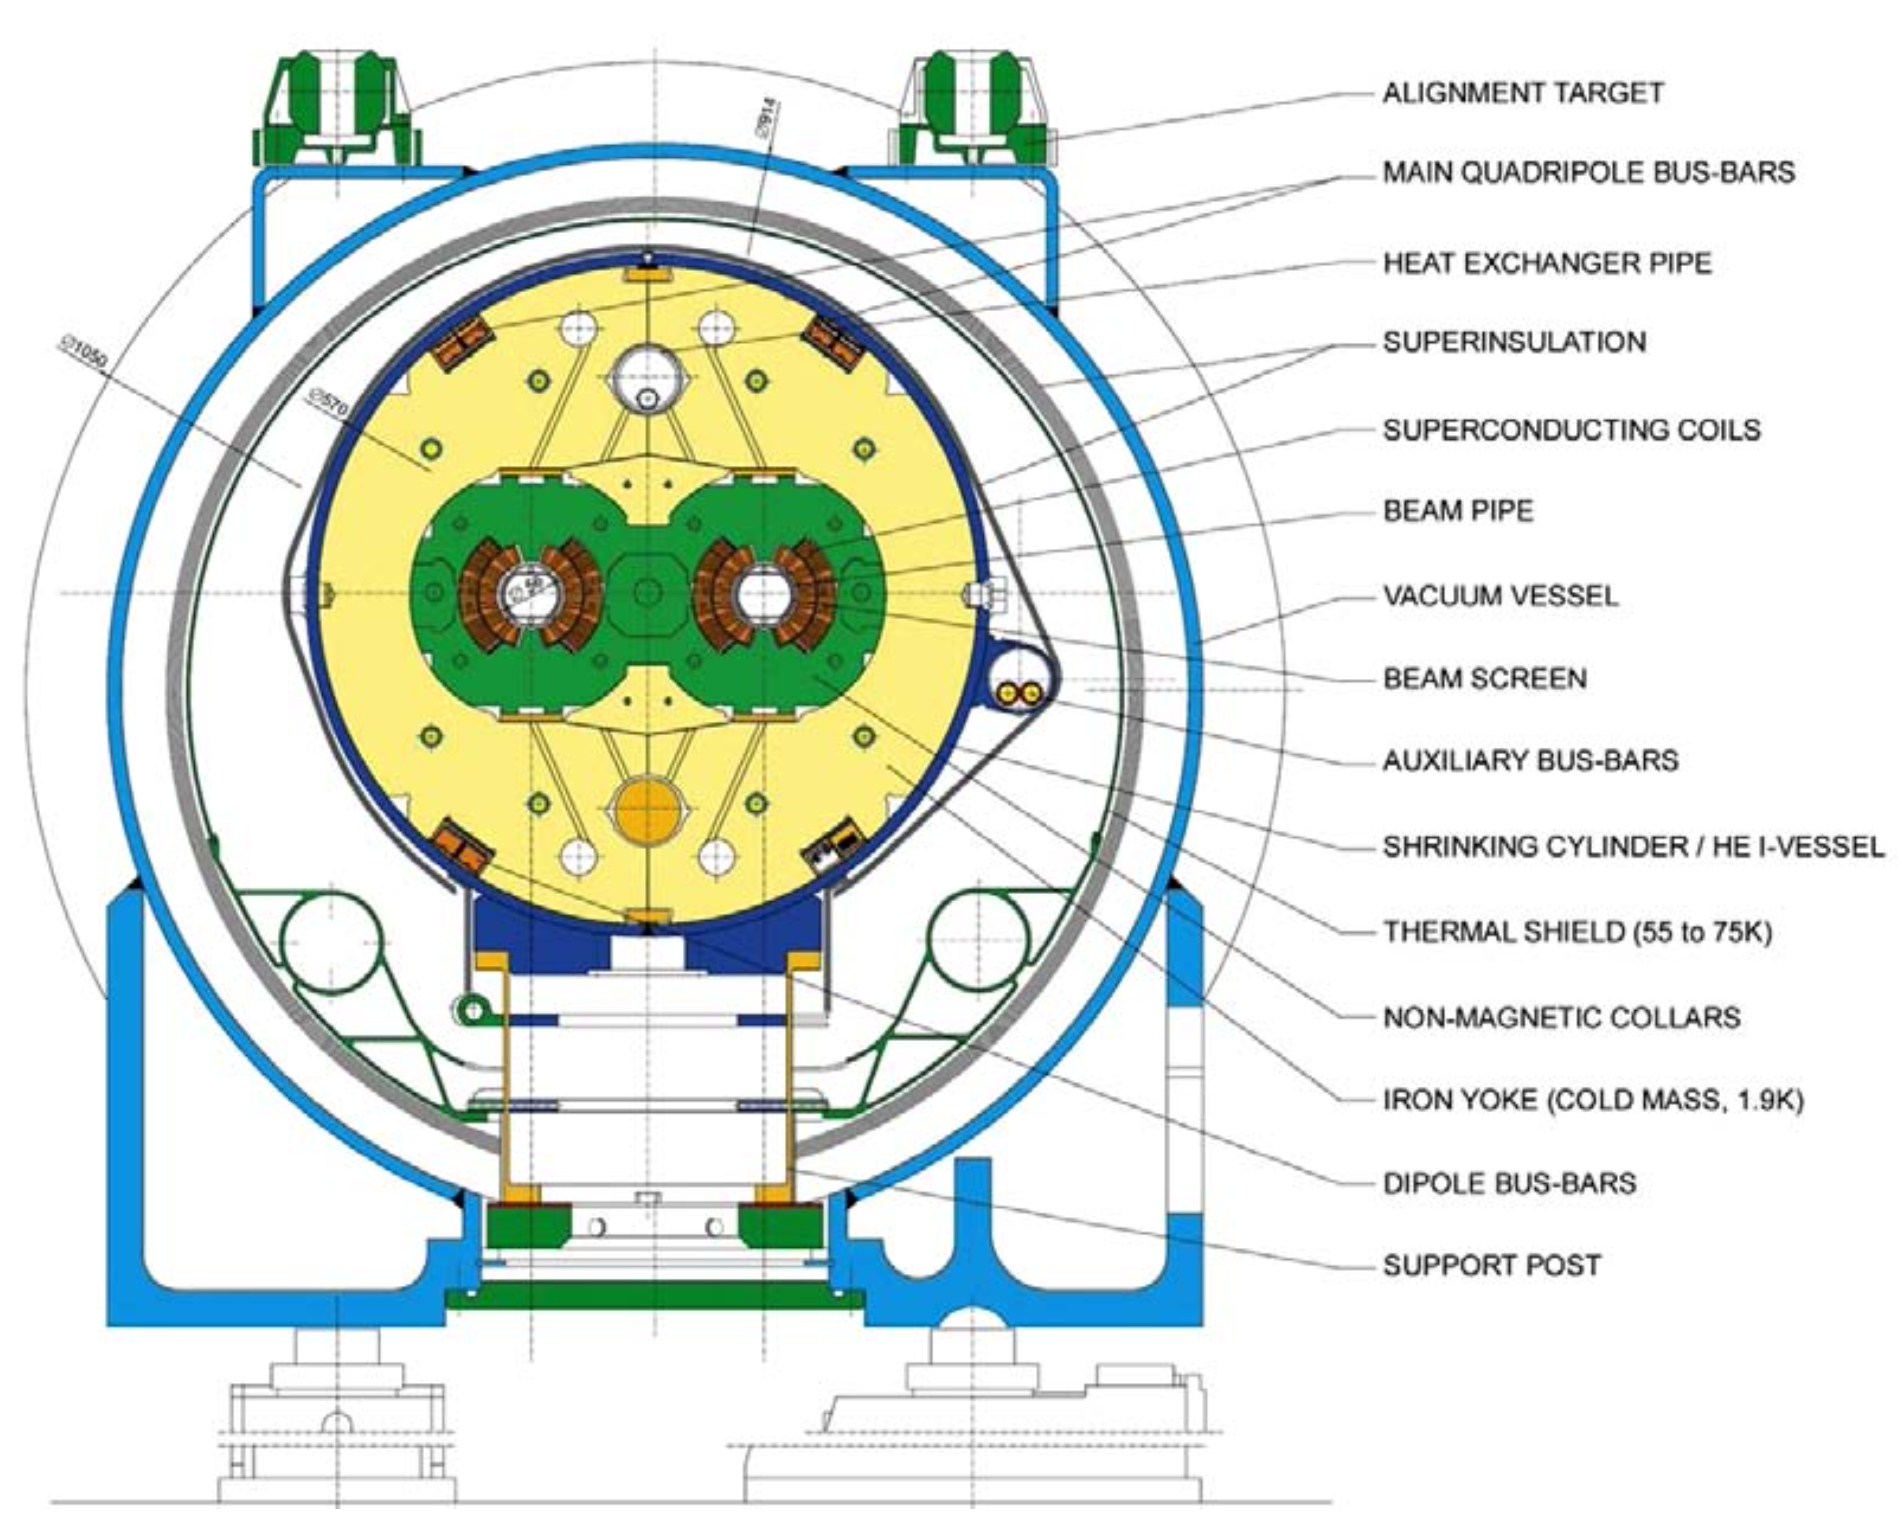
\includegraphics[width=\textwidth,keepaspectratio=true]{chapters/chapter2_experiment/images/dipole-crosssection.png}
		\caption{Cross-section of cryodipole (lengths in mm). \cite{lhc-machine}}
		\label{fig:dipole-xsec}
		\end{figure}

		\begin{figure}[!ht]
		\centering
		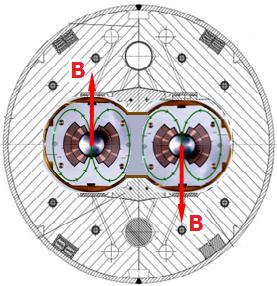
\includegraphics[width=.45\textwidth,keepaspectratio=true]{chapters/chapter2_experiment/images/dipole-field.jpeg}
		\caption{Field of the LHC dipole magnets. \cite{dipole-field}}
		\label{fig:dipole-field}
		\end{figure}

	\subsection{CERN Accelerator Complex}\label{ssec:cern-accelerators}
		There are a series of accelerators used to get each beam up to its final energy of 6.5 TeV. The protons used in collisions are sourced from hydrogen atoms. The hydrogen is ionized, leaving the nucleus consisting of one proton, these protons are then accelerated in radiofrequency (RF) cavities. Figure \ref{fig:CERN-complex} shows in detail the full accelerator complex at CERN.\footnote{Figure \ref{fig:CERN-complex} shows the newer LINAC 4 at the start of Run-3. This work is concerning data taken with LINAC 2.} 
		\begin{figure}[!ht]
		\centering
		\includegraphics[width=\textwidth,keepaspectratio=true]{chapters/chapter2_experiment/images/CERN-complex.png}
		\caption{The CERN accelerator complex. \cite{CERN-complex}}
		\label{fig:CERN-complex}
		\end{figure}
		The protons used in the LHC start the accelerating process in the linear accelerator LINAC 2. They then are accelerated in the booster, PS, SPS, and are finally injected at the LHC where they are accelerated to the final 6.5 TeV beam energy. The final energies of protons from each accelerator can be seen in Table \ref{tab:accelerator-complex}.
		\begin{table}[!thp]
			\centering
			\caption{Accelerator final energies}
			\begin{tabular}{| l | l |}  
			\hline
			Accelerator 					& Final Energy 	\\ \hline
			\hline
			LINAC 2 						& $50$ MeV 		\\ 	\hline
			Booster 						& $1.4$ GeV 	\\ 	\hline
			Proton Synchrotron (PS)			& $26$ GeV 		\\ 	\hline
			Super Proton Synchrotron (SPS) 	& $450$ GeV 	\\ 	\hline
			Large Hadron Collider (LHC)		& $6.5$ TeV 	\\ 	\hline
			\end{tabular}
			\label{tab:accelerator-complex}
		\end{table}

	\subsection{Luminosity}\label{ssec:lumi}
		The amount of data collected from colliders is often referred to in terms of luminosity. Luminosity is measured in terms of inverse barns, where $1 \, b = 10^{-28} \, m^2$. Instantaneous luminosity of one bunch crossing can be written as 
		\begin{equation}\label{eqn:bunch-lumi}
		\mathcal{L}_{bunch} = \frac{ \mu  f }{\sigma}
		\end{equation}
		where $\sigma$ is the cross section and can be thought of as the probability of a collision occurring, $\mu$ is the number of inelastic interactions per bunch crossing, and $f$ is the revolution frequency of the LHC $f=11246$ Hz. Therefore, the total instantaneous luminosity is 
		\begin{equation}\label{eqn:tot-inst-lumi}
		\mathcal{L} = N_b \frac{ \langle \mu \rangle f}{\sigma}
		\end{equation}
		where $\langle \mu \rangle$ is the average number of inelastic interactions per bunch crossing. 

		The integrated luminosity then corresponds to the total amount of data that was taken during a time period and can be seen for the LHC Run-2 in \ref{fig:lhc-lumi}
		\begin{figure}[!ht]
		\centering
		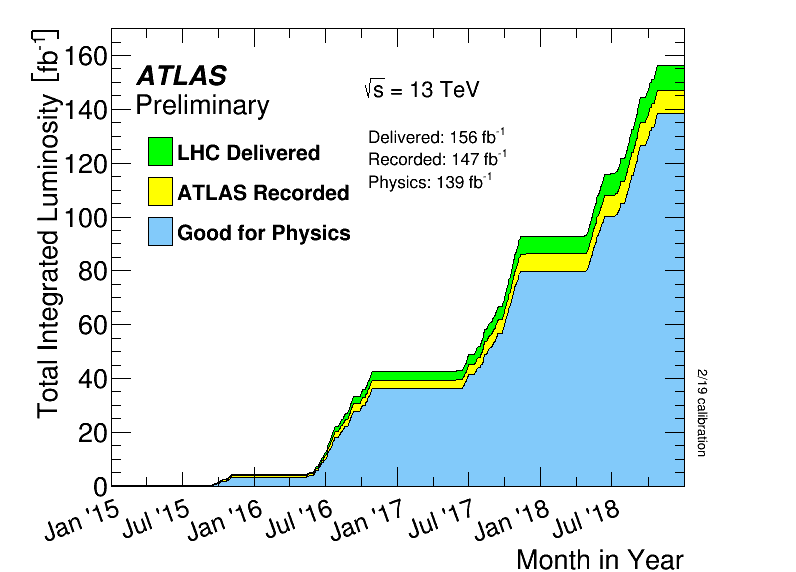
\includegraphics[width=.65\textwidth,keepaspectratio=true]{chapters/chapter2_experiment/images/intlumivstimeRun2DQall.png}
		\caption{ Cumulative luminosity versus time delivered to ATLAS (green), recorded by ATLAS (yellow), and certified to be good quality data (blue) during stable beams for pp collisions at 13 TeV center of mass energy in 2015-2018. The difference between the colored histograms reflects inefficiencies, especially those seen when restarting data taking. }
		\label{fig:lhc-lumi}
		\end{figure}
		The value of $\langle \mu \rangle$ changed throughout data taking and can be seen in Figure \ref{fig:run2-mu} and is referred to as pileup because the higher the $\langle \mu \rangle$ value, the more messy a collision becomes.
		\begin{figure}[!ht]
		\centering
		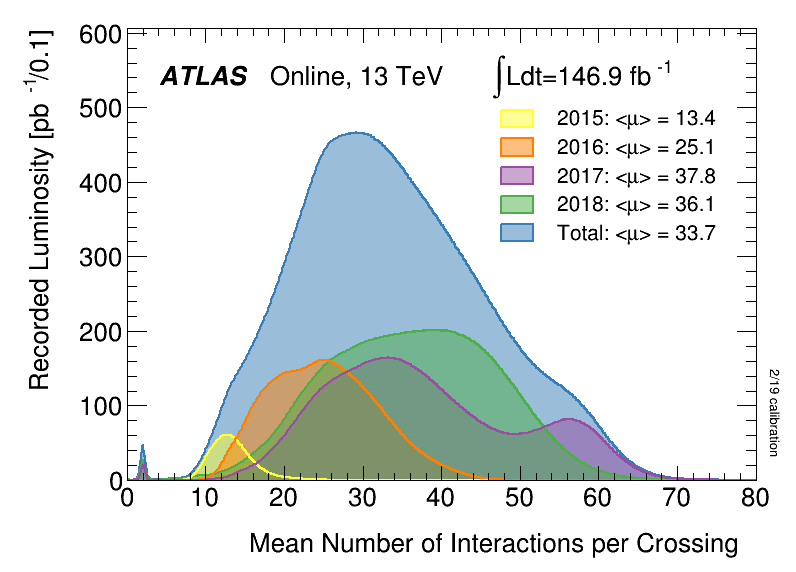
\includegraphics[width=.65\textwidth,keepaspectratio=true]{chapters/chapter2_experiment/images/mu_2015_2018.png}
		\caption{ The luminosity-weighted distribution of the mean number of interactions per bunch crossing for the 2015-2018 \pp collision dataset at $13$ TeV center of mass energy. }
		\label{fig:run2-mu}
		\end{figure}
		The effect of high pileup can be seen in Figure \ref{fig:high-pileup-event-display}, a collision event taken in 2018 with 29 reconstructed vertices shown on the bottom right as colored circles.
		\begin{figure}[!ht]
		\centering
		\includegraphics[width=\textwidth,keepaspectratio=true]{chapters/chapter2_experiment/images/event_display_r349114_e216445472_v4_wMoreTracks_v3_wAtlantisTrackColor_Inset.png}
		\caption{ A display of a candidate Z boson event from proton-proton collisions recorded by ATLAS with LHC stable beams at a collision energy of 13 TeV. The Z boson candidate is reconstructed in a beam crossing with 28 additionally reconstructed primary vertices from the minimum bias interactions. The candidate event is reconstructed in the 2$\mu$ final state. In the left display, the red lines show the path of the two muons including the hits in the muon spectrometer and the yellow tracks are the remaining charged particles from the 29 vertices, with transverse momentum above 0.5 GeV. The colored squares in the lower display correspond to the position of the reconstructed vertices. The invariant mass of the two muons is 92.3 GeV. }
		\label{fig:high-pileup-event-display}
		\end{figure}


		A common calculation using the total integrated luminosity is shown in Equation \ref{eqn:tot-proc-num}; where the number of times a particular process was produced is calculated.
		\begin{equation}\label{eqn:tot-proc-num}
		N_{x} = \mathcal{L} \sigma_{x}
		\end{equation}
		where again, $\sigma$ is the cross section. In this case, the cross section corresponding to process $x$.


\section{The ATLAS Detector}\label{sec:ATLAS}
	The ATLAS (\textbf{A} \textbf{T}oroidal LHC \textbf{A}pparatu\textbf{S}) detector is one of two general purpose particle detectors on the LHC. The other being the \textbf{C}ompact \textbf{M}uon \textbf{S}olenoid (CMS). ATLAS, like other particle detectors, is comprised of four main components; the inner detector, calorimeters, muon system, and the magnet system. Each component has several types of technology in order to measure the energy of all possible particle decays.\footnote{Neutrinos are not directly detected, but inferred via a missing transverse energy calculation described in Section \ref{sec:reco-etmiss}.} The full ATLAS detector measures 44 m in length, 25 m in diameter, and weighs over 7000 tonnes. Figure \ref{fig:ATLAS} shows a 3D model of the ATLAS detector and Figure \ref{fig:ATLAS-XSec} shows a cross section of the detector and various particles trajectory.\footnote{Figure \ref{fig:ATLAS} shows the New Small Wheel muon-chambers. This dissertation concerns data collected with the old Small Wheel muon-chambers.} All of the subdetectors output data to the Trigger and Data Acquisition (TDAQ) system that selects collisions with interesting physics using a complex mix of hardware and software algorithms detailed in \ref{ssec:trigger}. 

	\begin{figure}[!ht]
	\centering
	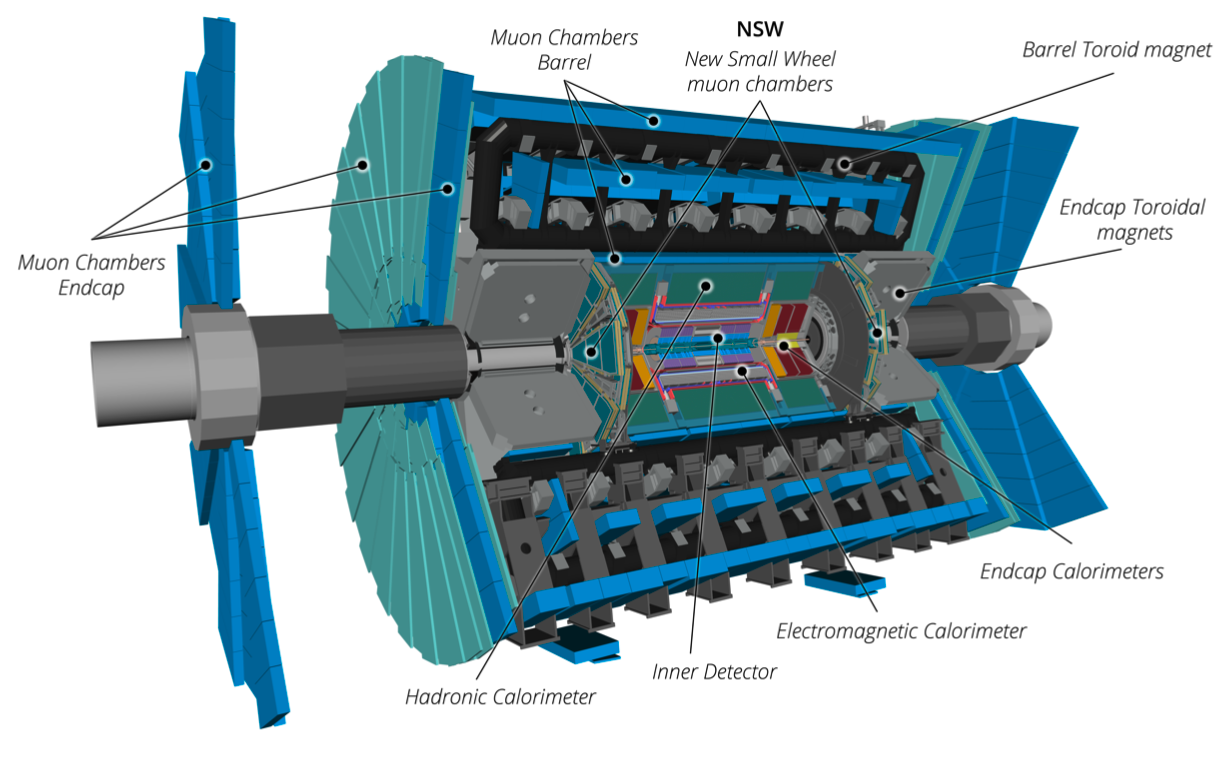
\includegraphics[width=.75\textwidth,keepaspectratio=true]{chapters/chapter2_experiment/images/ATLAS_3d_run3.png}
	\caption{ Cut-away view of the ATLAS detector with major subdetectors highlighted.}
	\label{fig:ATLAS}
	\end{figure}

	\begin{figure}[!ht]
	\centering
	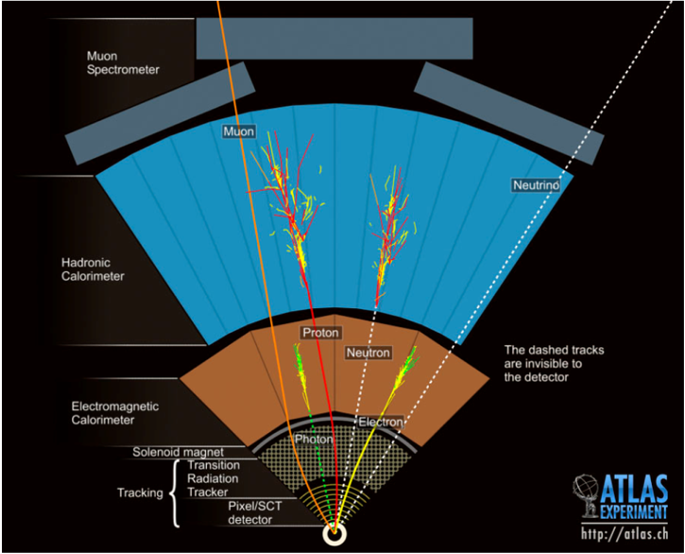
\includegraphics[width=.65\textwidth,keepaspectratio=true]{chapters/chapter2_experiment/images/ATLASCrossSectionDiagram.png}
	\caption{ Cross section view of the ATLAS detector with subdetectors labeled. Various types of particles radial trajectories are shown.}
	\label{fig:ATLAS-XSec}
	\end{figure}

	\subsection{Detector Coordinates}\label{ssec:coordinates}
	Since ATLAS is a cylinder, it is convenient to start with polar cylindrical coordinates. For ATLAS, the z-axis is inline with the beam line, the x-axis points towards the center of the LHC ring, and the y-axis points vertically. However, since particle collisions are relativistic by nature, a set of Lorentz invariant coordinates is much more useful. The radial coordinate r defines the radial distance from the interaction point (IP) at the center of ATLAS, $\phi$ is the azimuthal angle describing the angle from the x-axis in, and $\eta$, the pseudorapidity, is defined as 
	\begin{equation}\label{eqn:eta}
	\eta \equiv - ln(tan(\frac{\theta}{2}))
	\end{equation}
	where $\theta$ is the angle from the y-axis. It is in the differences in $\eta$ between particles that provides the Lorentz invariance in this coordinate system of $(r,\phi,\eta)$. Due to the large collision energies of the LHC, the pseudorapidity is a close estimate to the true rapidity of the particles. 
	\begin{equation}\label{eqn:rapidity}
	y \equiv \frac{1}{2} ln(\frac{E+p_Z}{E-p_Z}) \approx \eta
	\end{equation}
	When speaking of differences in particle locations within ATLAS, $\Delta R$  is often used.
	\begin{equation}\label{eqn:dR}
	\Delta R \equiv \sqrt{ (\Delta \eta)^2 + (\Delta \phi)^2}
	\end{equation}

	% In the ATLAS detector, the central barrel section corresponds to $|\eta| < 2.5$
	Figure \ref{fig:pseudorapidity} shows visually how $\eta$ relates to $\theta$. In the ATLAS detector, the central barrel section corresponds to a range of $|\eta|<1$. 

	\begin{figure}[!ht]
	\centering
	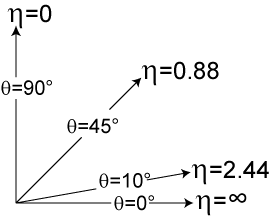
\includegraphics[width=.25\textwidth,keepaspectratio=true]{chapters/chapter2_experiment/images/Pseudorapidity.png}
	\caption{ A diagram showing the pseudorapidity $\eta$ and corresponding $\theta$ values. \cite{pseudorapidity} }
	\label{fig:pseudorapidity}
	\end{figure}

	\subsection{Magnet Systems}\label{ssec:magnets}
	The ATLAS detector makes use of two superconducting magnet systems; a central solenoid and a toroid system. Both systems provide large magnetic fields to curve charged particles. The curvature can be used to measure the electromagnetic charge and charge to mass ratio, effectively measuring the momentum of charged particles. Figure \ref{fig:ATLAS-magnets} shows the magnets in ATLAS.

	\begin{figure}[!ht]
	\centering
	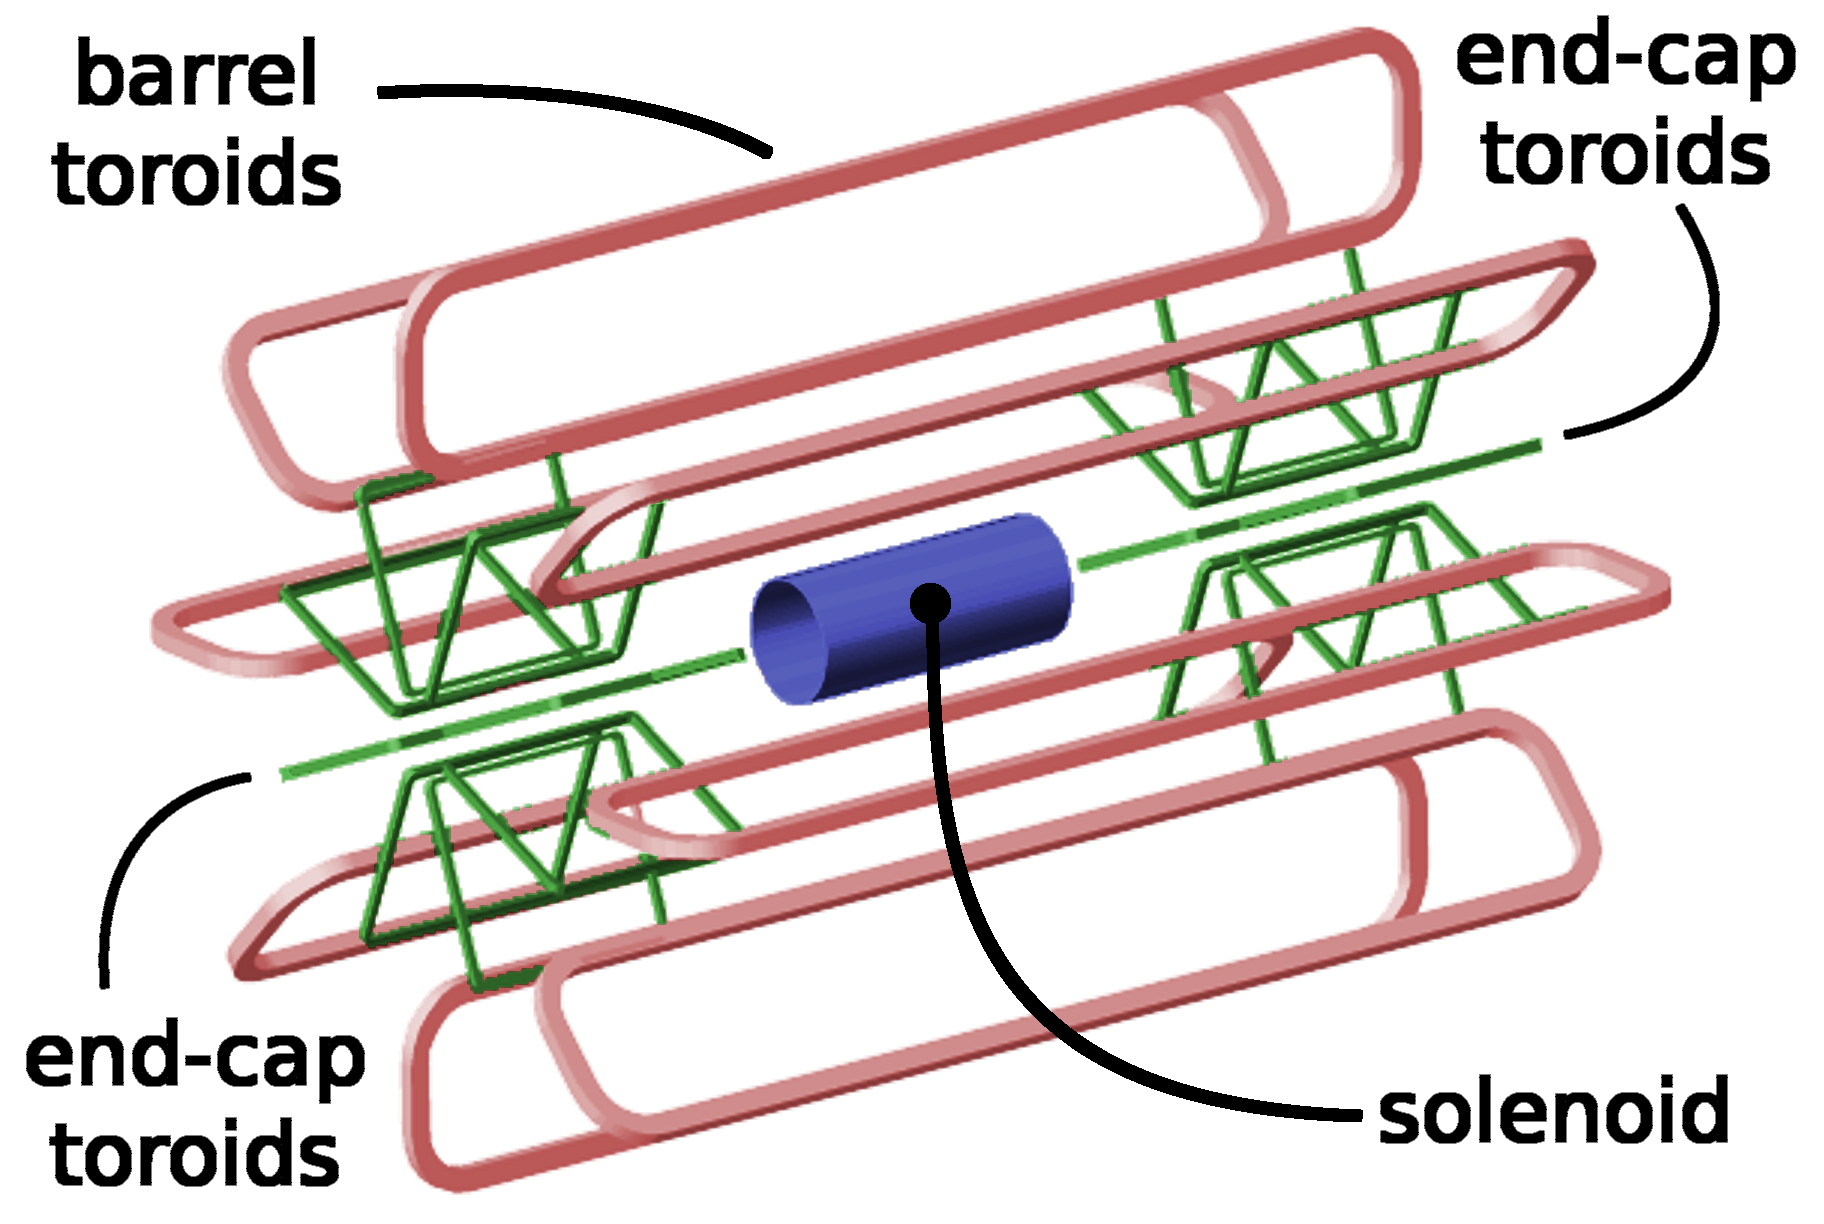
\includegraphics[width=.65\textwidth,keepaspectratio=true]{chapters/chapter2_experiment/images/magnetSystems.png}
	\caption{ The ATLAS magnet systems.}
	\label{fig:ATLAS-magnets}
	\end{figure}

	\subsubsection{Solenoid System}\label{sssec:solenoid}
	The central solenoid encases the Inner Detector (ID), creating an axially symmetric 2 T magnetic field. This magnetic field bends charged particles in the transverse plane throughout the ID. The solenoid magnet itself measures 5.3 m in length and 2.63 m in diameter. In an effort to decrease the amount of material in front of the calorimeters the solenoid magnet was made to be thin. It is a single-layer coil with approximately 1200 turns of NbTi superconducting wires encased in Al-Cu to structurally stabilize the magnet material \cite{atlas-solenoid}. The steel structure within the Tile calorimeter acts as the magnetic flux return for the solenoid magnet system. 70\% of this flux passes through the supporting girder structure, 25\% through the active calorimeter material, and roughly 2\% through the front-plates of the Tile calorimeter \cite{ATLAS-tile}.

	\subsubsection{Toroid System}\label{sssec:toroid}
	The ATLAS detector gets its name from the toroid magnetic system that is critical in the identification of high energy muons. The toroid system bends any charged particles that make it past the calorimeters along the beam axis. This is achieved through a radially symmetric magnetic field of 3.9 T in the barrel and 4.1 in the end-caps. The barrel toroid system is comprised of 8 air core superconducting toroid magnets that each measure 25 m in length, 10 m in diameter, and weigh 750 tonnes. The superconducting wires are the same used in the solenoid, NbTi encased in Al-Cu \cite{atlas-toroid}. Each magnet is encased in a stainless steel cryogenic chamber, or cryostat. The toroid magnet system has two end-cap toroids that are very similar in construction to the barrel toroids. The end-cap toroids also have 8 coils measuring 5 m in length and 10 m in diameter. Instead of individual cryostats for each coil, the end-caps are encased in large cryostats that hold all 8 coils. This allows the end-caps to be pulled out and offers easy access to the rest of the detector. Just like with the central solenoid system, the design of the toroid system was chosen to limit the amount of material between detector components. A solenoid magnet of similar size to the toroid system would not only add more material, but would be cost prohibitive as well.


	\subsection{Inner Detector}\label{ssec:ID}
		\begin{figure}[!ht]
		\centering
		\subfloat[\label{fig:hpm-diagrams_a}]{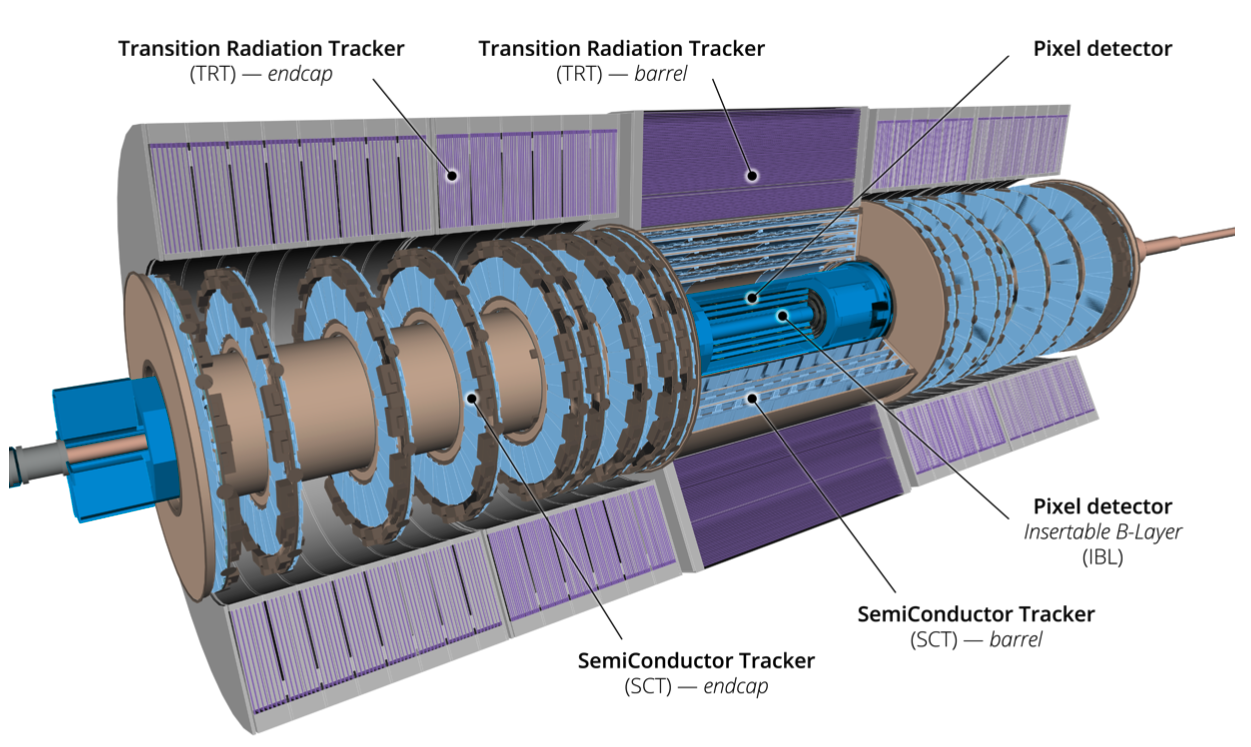
\includegraphics[width=.55\textwidth,keepaspectratio=true]{chapters/chapter2_experiment/images/ATLAS_ID_Run3.png}}
		\subfloat[\label{fig:hpm-diagrams_b}]{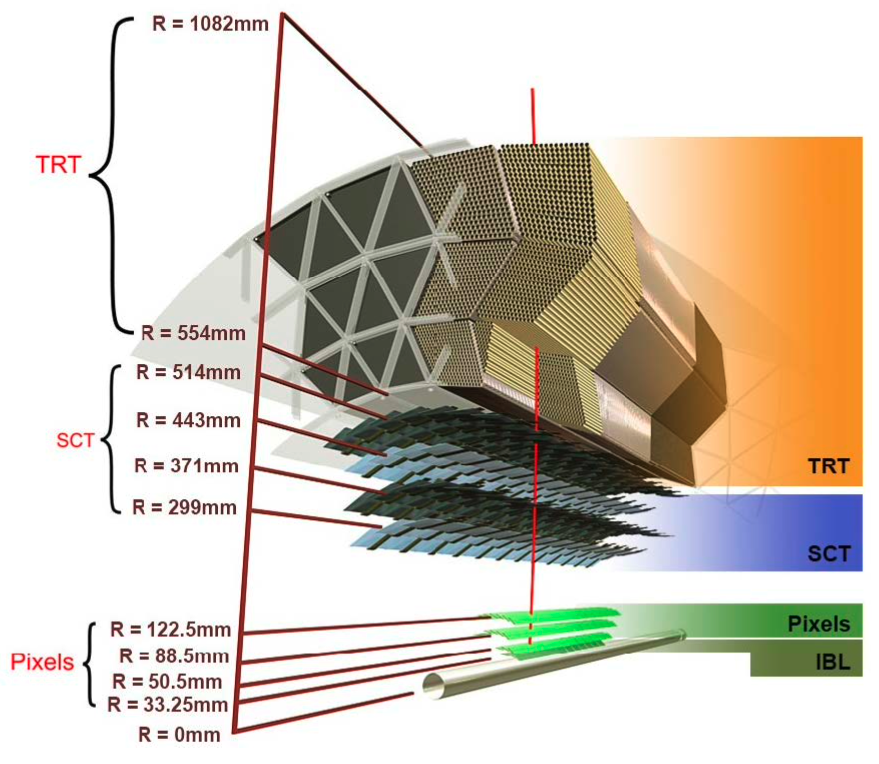
\includegraphics[width=.45\textwidth,keepaspectratio=true]{chapters/chapter2_experiment/images/ATLAS_ID_Transverse_View.png}}
		\caption{\label{fig:ATLAS-ID} (a) Cut-away view of the ATLAS Inner Detector. (b) Cross-sectional view of the ATLAS Inner Detector.}
		\end{figure}

		The ID is the inner-most detector, closest to the IP and is used to track the trajectory of charged particles leading to the measurement of electromagnetic charge and momentum. The ID is immersed in the 2 T magnetic field provided by the central solenoid described in section \ref{sssec:solenoid} and covers a pseudorapidity range of $|\eta|<2.5$. The three subdetectors within the ID can be seen in Figure \ref{fig:ATLAS-ID}, the Pixel, \textbf{S}emi\textbf{C}onductor \textbf{T}racker (SCT), and the \textbf{T}ransition \textbf{R}adiation \textbf{T}racker (TRT). Like the toroid system, and many of the other subdetectors, the ID is comprised of barrel and end-cap segments. The ID barrel section is 1.6 m in length and covers $|\eta|<1$ while the end-caps measure over 7 m in length and cover $1 < |\eta| < 2.5$. 

		A track is considered good if there are hits in at least 3 pixel layers and 8 strips. The ID tracking system was designed with a resolution of 
		\begin{equation}\label{eqn:tracking-resolution}
		\frac{\sigma_{\pt}}{\pt} = 0.05 \% \, \pt \oplus 1\%
		\end{equation}
	
		\subsubsection{Pixel}\label{sssec:pixel}
		The detector closest to the beam and IP is the Pixel Detector. The Pixel Detector is designed to measure with high-precision and high-granularity. The barrel Pixel detector consists of three layers of n-type silicon substrate with n-type implants. The closest layer to the IP sits at 50.5 mm and the outermost layer extends out to 12 cm. This combination gives the Pixel Detector the ability to determine the impact parameters of collisions with incredible precision. Due to the high radiation dose this close to the IP, the Pixel Detector was designed to be operated only in partial depletion. Each pixel cell measures $200 \mu m \times 400 \mu m \times 250 \mu m$. There are five Pixel disks on each end-cap of the ID. In total there are 1,744 modules, 46,080 readout channels per module, giving over 80 million channels with a spatial resolution of $10 \, \mu m (R-\phi) \times 115 \, \mu m (z)$ \cite{ATLAS-pixel}. 

		In order to keep up with the increased demand of Run-2 data taking conditions, an additional layer of pixels was installed in the Long Shutdown 1 (LS1) between 2013 and 2015. This \textbf{I}nsertable \textbf{B} \textbf{L}ayer (IBL) provides even finer granularity tracking with pixel cells measuring $50 \, \mu m \times 250 \, \mu m$ installed at a radial distance of $R=33.25$ mm from the IP and a spatial resolution of $8 \, \mu m (R-\phi) \times 40 \, \mu m (z)$ \cite{ATLAS-IBL}. The IBL has proved incredibly useful in the reconstruction of displaced vertices from processes like \bjet hadronization and $\gamma \rightarrow e^+ e^-$.

		\subsubsection{Semiconductor Tracker}\label{sssec:SCT}
		Moving radially outward, the next subdetector is the SCT that provides tracking in the intermediate radial range from the IP and covers a range of $|\eta| < 2.5$. Similar to the Pixel Detector, the SCT has 4 barrel layers and 9 end-cap wheels on each side. The SCT provides four measurements per track via silicon microstrip detectors. Each microstrip is made of two $6.36 \times 6.40 \, cm^2$ detectors glued end to end so each microstrip is $12.8 \, cm$ long. Two microstrips are then glued back to back with a $40 \, \mu rad$ angle. In total there are 768 strips, giving 6.2 million readout channels. The SCT has a spatial resolution of $17 \, \mu m (R-\phi) \times 580 \,\mu m (z)$ and can distinguish tracks with as small as a $200 \, \mu m$ separation \cite{ATLAS-ID}.

		\subsubsection{Transition Radiation Tracker}\label{sssec:TRT}
		The final subdetector of the ID is the TRT $(R=554 \, \mathrm{mm} \, - 1082 \, \mathrm{mm})$ . Instead of silicon detectors the TRT uses 4 mm diameter straw tubes; a hollow tube with a sense wire held at high voltage in the middle. The max length of a straw is 150 cm. The straws are filled with a gaseous mixture of $70\% \, \mathrm{Xe,} \, 27\% \, \mathrm{CO}_2, \, 3\% \, \mathrm{O}_2$.\footnote{During Run-2 the Xe was replaced with Ar as a cost saving measure. Ar provides similar performance as Xe in tracking, but is less efficient in absorbing X-rays from transition radiation.} Charged particles ionize the gas mixture, thereby releasing an electron and an ion. The ion drifts to the straw surface and the electron drifts to the wire; this charge drift is then measured as a signal. The TRT checks the signals against two thresholds, a lower threshold for measuring the drift time to derive a position and a higher threshold that is used to identify transition radiation X-rays. The higher threshold provides discriminating power between charged pions and electrons.

		The TRT consists of a barrel section and 18 wheels in each end-cap. In the barrel, there are 50,000 straws divided in two at the center to allow for two separate readouts. The end-caps have 320,000 straws. In total, there are 420,000 readout channels. Each straw provides a spatial resolution of $170 \mu m$. \cite{ATLAS-ID}

	\subsection{Calorimeters}\label{ssec:calorimeters}
	The ATLAS detector makes use of two types of sampling calorimeters, one that uses liquid argon as the active medium and another that uses scintillating plastic tiles. Both types of calorimeters are designed to fully absorb particles via showering. Incoming particles interact with an absorber material and generate secondary particles. Those secondary particles interact with the absorber and create another set of particles. This cascading effect creates showers of particles inside the calorimeters. The shape and depth of these particles is important in the design choices for the calorimeters as well as particle identification. Two helpful variables when talking about shower depth are radiation length $\chi_0$ and nuclear interaction length $\lambda$. $\chi_0$ is defined as the distance where a particle has lost energy via bremsstrahlung equal to $\frac{1}{e}$.\footnote{$\chi_0$ can also be defined as $\frac{7}{9}$ of the mean free path of a high energy photon.} Whereas $\lambda$ is the mean free path of a hadron before undergoing a inelastic nuclear interaction. In order to fully absorb a wide energy range of incident particles the calorimeters are such that any path through them is at least $25 \, \chi_0$ or $10 \, \lambda$. Figure \ref{fig:calo-interaction-length} shows the calorimeters and their nuclear interaction lengths as a function of $\eta$.

	\begin{figure}[!ht]
	\centering
	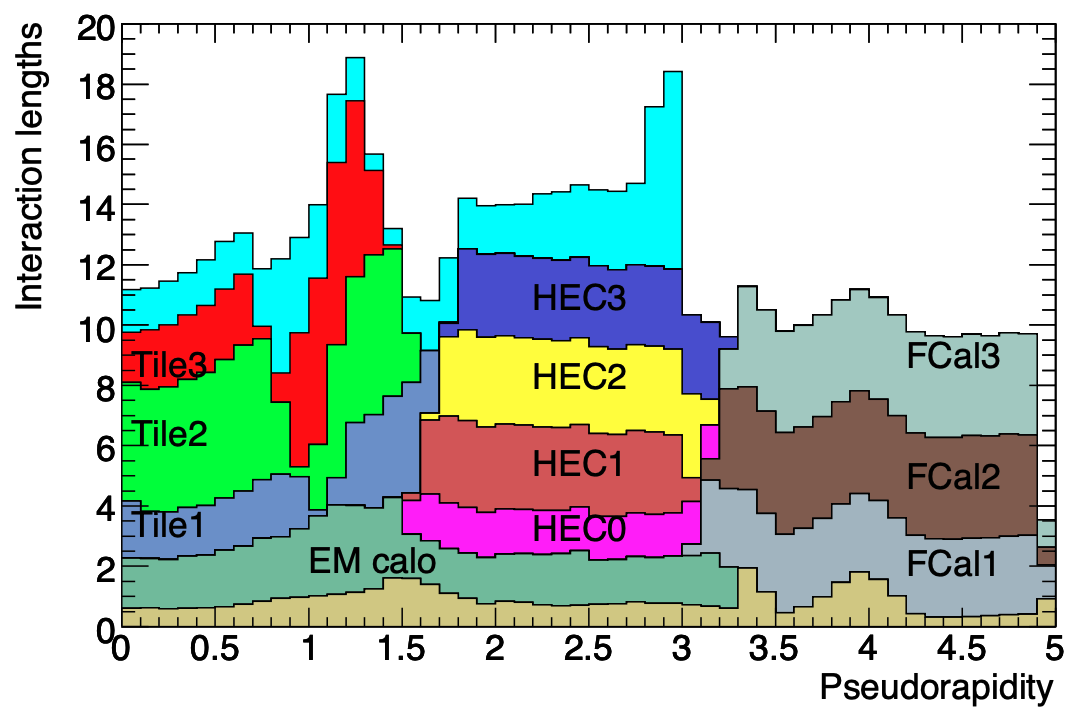
\includegraphics[width=.65\textwidth,keepaspectratio=true]{chapters/chapter2_experiment/images/Calo_Interaction_Lengths.png}
	\caption{ Interaction lengths as a function of $\eta$ in the ATLAS calorimeters. The unlabeled brown color is the material in front of the EM calorimeters and the unlabeled cyan is the amount of material in front of the first active layer of the muon spectrometer. \cite{atlas-experiment}}
	\label{fig:calo-interaction-length}
	\end{figure}

	The design resolution of the calorimeters can be seen in Table \ref{tab:calo-resolution}.

	\begin{table}[!thp]
	\centering
	\caption{ Design resolution of EM and hadronic calorimeters in the ATLAS Detector.}
	\resizebox{.45\textwidth}{!}{\begin{tabular}{| c | c | c |}  
	\hline
	Calorimeter											& Pseudorapidity range 																		& Resolution \\[1ex] \hline 
	Electromagnetic 									& $| \eta | < 3.2$ 																			& $\frac{\sigma}{E} = \frac{10\%}{\sqrt{E}} \oplus 0.7\%$ \\[1ex] \hline
	\multicolumn{1}{|c|}{\multirow{2}{*}{Hadronic}} 	& \begin{tabular}[c]{@{}c@{}} $| \eta | < 3.2$ \\[1ex] $3.1 < | \eta | < 4.9$ \end{tabular} & \begin{tabular}[c]{@{}c@{}} $\frac{\sigma}{E} = \frac{50\%}{\sqrt{E}} \oplus 3\%$ \\[1ex] $\frac{\sigma}{E} = \frac{100\%}{\sqrt{E}} \oplus 10\%$ \end{tabular} \\ \hline 
	\end{tabular}}
	\label{tab:calo-resolution}
	\end{table}

	The layout of calorimeters in the ATLAS detector can be seen in Figure \ref{fig:calo-layout}.
	\begin{figure}[!ht]
	\centering
	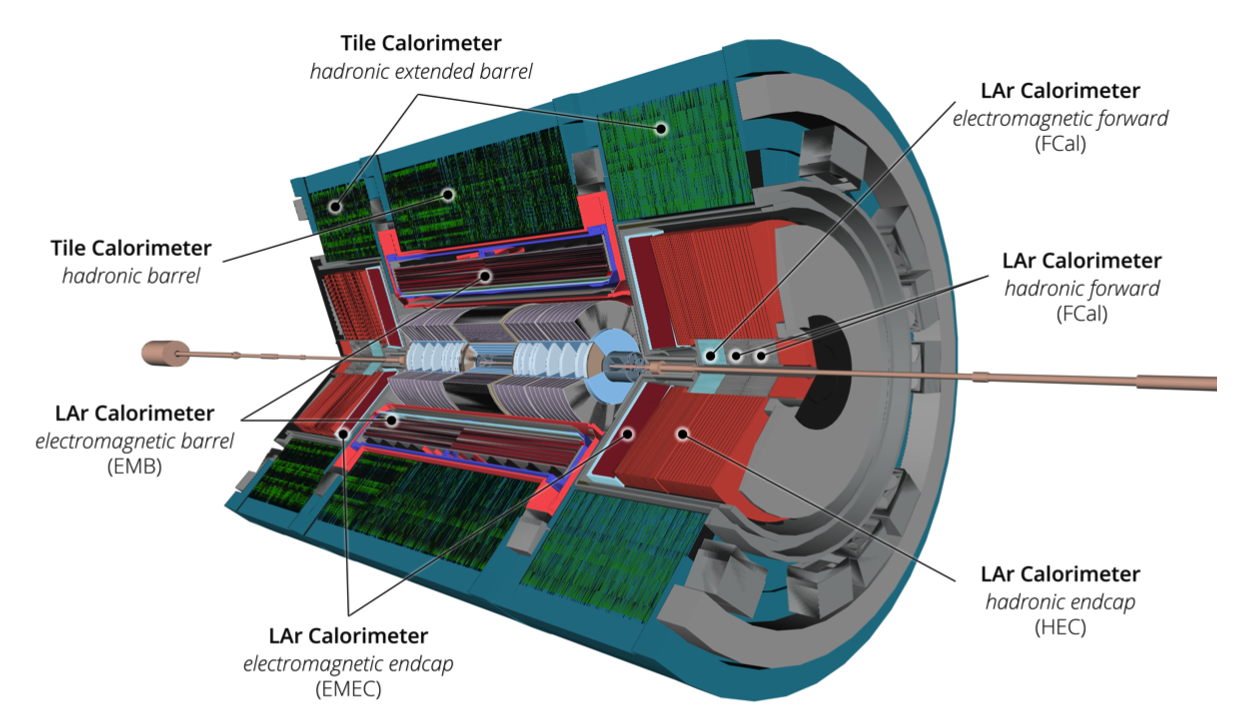
\includegraphics[width=.65\textwidth,keepaspectratio=true]{chapters/chapter2_experiment/images/ATLAS_Calorimeters_Run3.png}
	\caption{ Cut-out view of the ATLAS detector's calorimeters.}
	\label{fig:calo-layout}
	\end{figure}

		\subsubsection{Liquid Argon Calorimeters}\label{sssec:LAr}
		A liquid argon (LAr) is based on a similar principle to the straw tubes of the TRT described in section \ref{sssec:TRT}. In this case, the LAr is the active medium that is ionized by the incoming particle. The free electron then drifts to an electrode, copper-tungsten in the case of the barrel LAr calorimeter. The drifting electrons are then readout as an electrical signal; there are approximately 180,000 LAr readout channels in the ATLAS detector. LAr was chosen as the active medium due to it's intrinsic radiation hardness, stability over time, and linear response. The LAr must be kept at very cold temperatures, around 85 K. To achieve this, the LAr calorimeters are kept in cryostats, the barrel calorimeter shares the cryostat and vacuum with the central solenoid.

		There are four LAr calorimeters within the ATLAS detector. The main barrel section (EMB) is designed for electromagnetic calorimetry with a lead-stainless steel absorber and covers a pseudorapidity range of $|\eta|<2.5$. Next in $\eta$ is the LAr Electromagnetic End-Cap (EMEC) that also uses lead-stainless steel absorber and the LAr Hadronic End-Cap (HEC) which has a copper plate absorber; both EMEC and HEC cover $1.5 < |\eta| < 3.2$. The final LAr calorimeter is the aptly named Forward Calorimeter (FCAL) that covers $|\eta|<4.9$ and has three modules. The first is optimized for EM calorimetry and uses a copper absorber. The other two FCAL modules are used to measure hadronic showers and use tungsten absorbers.

		The EMB and EMEC both utilize an accordion geometry pictured in Figure \ref{fig:LAr-accordion} to ensure a full $\phi$ coverage. 
		\begin{figure}[!ht]
		\centering
		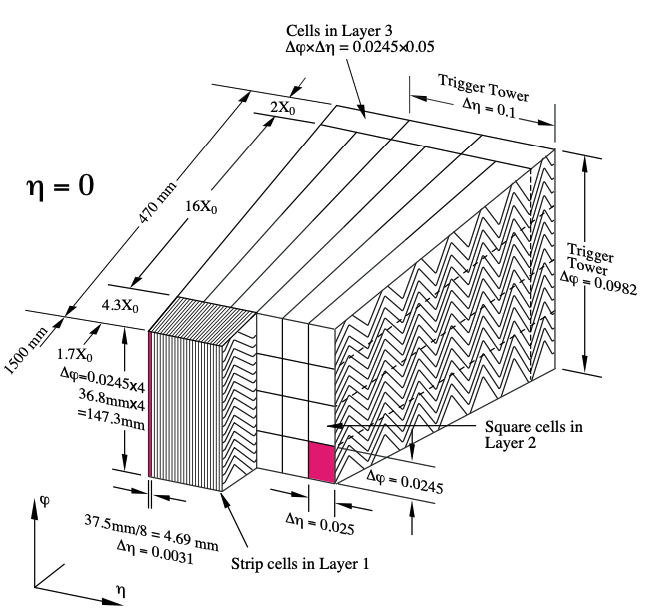
\includegraphics[width=.45\textwidth,keepaspectratio=true]{chapters/chapter2_experiment/images/LAr_Accordion_Geometry.png}
		\caption{ A EMB module showing the accordion geometry and granularity. \cite{atlas-experiment}}
		\label{fig:LAr-accordion}
		\end{figure}
		The EMB consists of four layers, the first being a LAr presampler of 1.1 cm thickness. The presampler is used to correct for energy losses due to material in front of the calorimeter. The first layer after the presampler is finely segmented to ensure good position measurements. The second layer is $16 \, \chi_0$ thick and collects most of the electromagnetic showers. Typically, only the tails of EM showers make it to the third and final layer, so a courser granularity is used. 

		\subsubsection{Tile Calorimeter}\label{sssec:Tile}
		\begin{figure}[!ht]
		\centering
		\subfloat[\label{fig:tile-modules_a}]{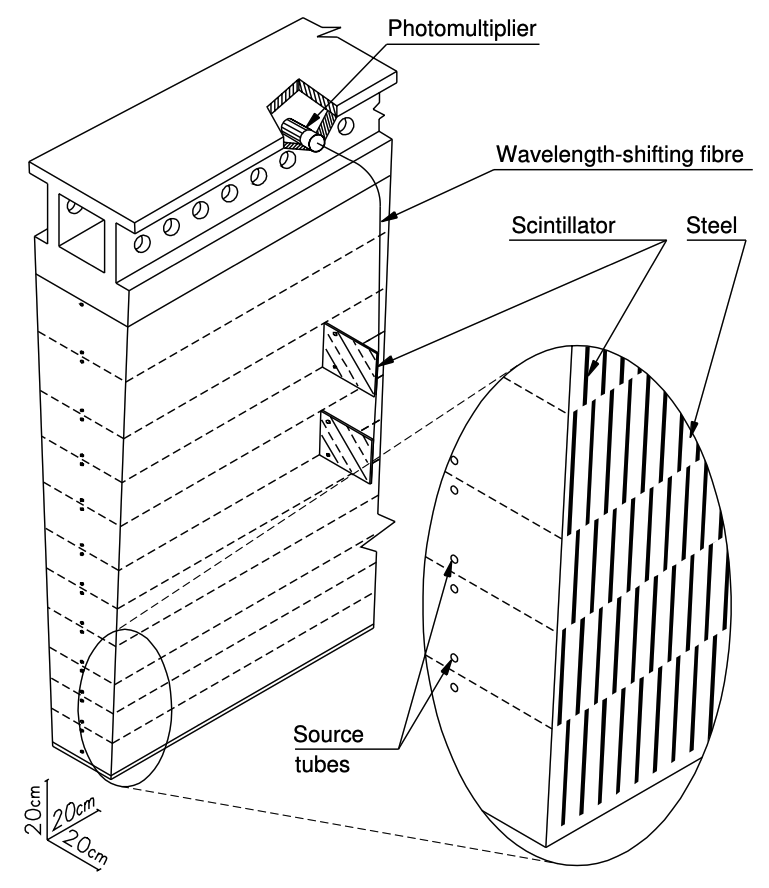
\includegraphics[width=.45\textwidth,keepaspectratio=true]{chapters/chapter2_experiment/images/TileModuleCrossSection.png}} \\
		\subfloat[\label{fig:tile-modules_b}]{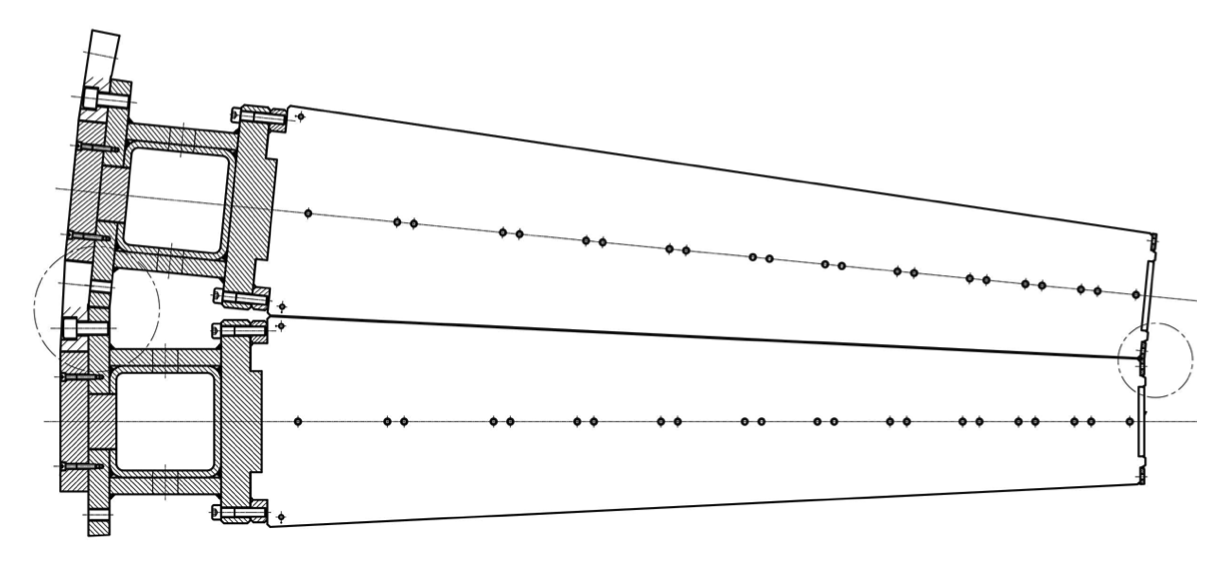
\includegraphics[width=.45\textwidth,keepaspectratio=true]{chapters/chapter2_experiment/images/Tile_Modules_Azimuth_View.png}}
		\caption{\label{fig:tile-modules} (a) Diagram of an individual TileCal module. (b) Azimuthal view of two TileCal modules with the IP being to the right.}
		\end{figure}
		The hadronic Tile Calorimeter (TileCal) is a sampling calorimeter that is designed to fully absorb hadronic showers covering a range of $|\eta|<1.7$ at a radial distance of $2.28 \, \mathrm{m} \leq R \leq 4.25 \, \mathrm{m}$ from the IP. This radial distance translates to approximately $7.4\, \lambda$. A similar design of absorber and electrode is used in TileCal to capture the full energy of hadronic showers. TileCal uses a steel absorber. However, instead of a liquid or gas being ionized and the free electrons being collected as a signal, TileCal takes advantage of a special material called scintillating plastic. When an ionizing particle interacts with the scintillating plastic, light is created; this light is absorbed in wavelength shifting (WLS) fibers. It is then re-emitted and transmitted to photomultiplier tubes (PMTs). The PMT signal is then shaped, amplified at two gains with a ratio of 64:1, then digitized at 40 MHz with 10-bit analogue-to-digital converters (ADCs). Each cell within TileCal has 2 PMTs, giving over 10,000 readout channels. There are 256 modules within TileCal. A diagram of an individual module and the layout of two modules side-by-side can be seen in Figure \ref{fig:tile-modules}.
		

		A significant fraction of the author's time and effort during their PhD went to data quality monitoring and maintenance of TileCal. These works are detailed in Appendix \ref{app:Tile-DQ}.

	\subsection{Muon Spectrometer}\label{ssec:muon-system}
	High momentum muons provide a vital signature at the LHC. Muons are minimally ionizing particles, meaning they leave a small amount of energy inside detectors and travel to the edge and beyond the volume of the ATLAS detector. Instead of attempting to fully absorb muons, high precision position measurements are taken to track their trajectories. The toroid magnet system described in section \ref{sssec:toroid} is an integral part of the Muon Spectrometer; it provides the bending force, changing the trajectories to the direction of the beamline. The barrel section of the Muon Spectrometer consists of three concentric cylindrical shells at $R=5 \, \mathrm{ m, }\, 7.5 \, \mathrm{ m, } \,  10 \, \mathrm{ m}$ made of Monitored Drift Tubes (MDTs) $(|\eta|<1)$. \cite{ATLAS-muon} These cylindrical shells sit in-between and on the air core toroid magnets. On the $2^{\mathrm{nd}}$ and $3^{\mathrm{rd}}$ shells are Resistive Plate Chambers (RPCs) that provide quick triggering. Complimenting the barrel section are the end-caps, referred to as wheels for the Muon Spectrometer. The wheels are placed at $|z|\approx 7.4 \, \mathrm{ m, } \, 10.8 \, \mathrm{ m, } \, 14 \, \mathrm{ m, and} \,21.5 \,\mathrm{ m }$ $(2.0 < |\eta| < 2.7)$. The innermost layer of these wheels experience the highest rates of incident particles. To cope with this, Cathode Strip Chambers (CSCs) with a finer granularity than the MDTs that are used in the barrel. Similarly, Thin Gap Chambers (TGCs) are used for triggering instead of RPCs. These wheels provide spatial coordinates orthogonal to those of the precision-tracking MDTs in the barrel. Figure \ref{fig:muon-spec} shows the positioning of the various Muon Spectrometer components.\footnote{Figure \ref{fig:muon-spec} Shows the New Small Wheel (NSW). The NSW is an upgrade to the old Small Wheels that were used in the data taking period that concerns this dissertation.}

	% \begin{figure}[!h]
	% \centering
	% \subfloat[\label{fig:muon-spec_a}]{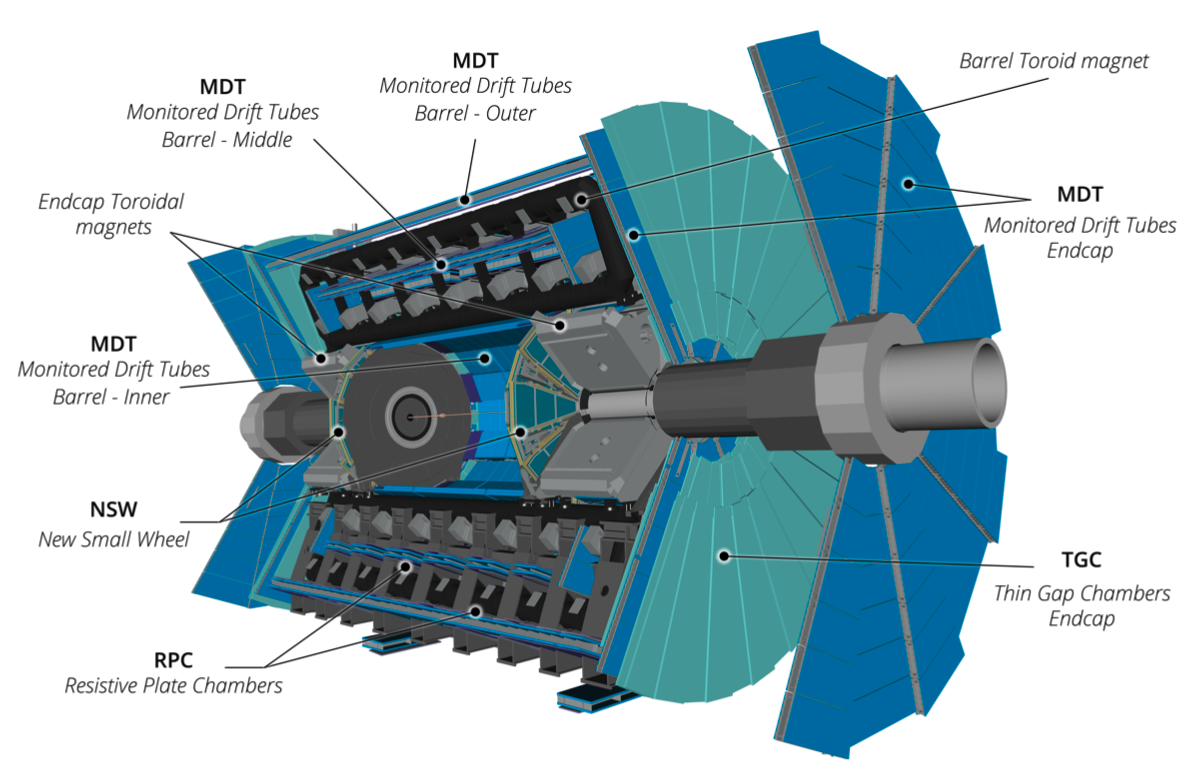
\includegraphics[width=.45\textwidth,keepaspectratio=true]{chapters/chapter2_experiment/images/ATLAS_Muon_System_Run3.png}}
	% \subfloat[\label{fig:muon-spec_b}]{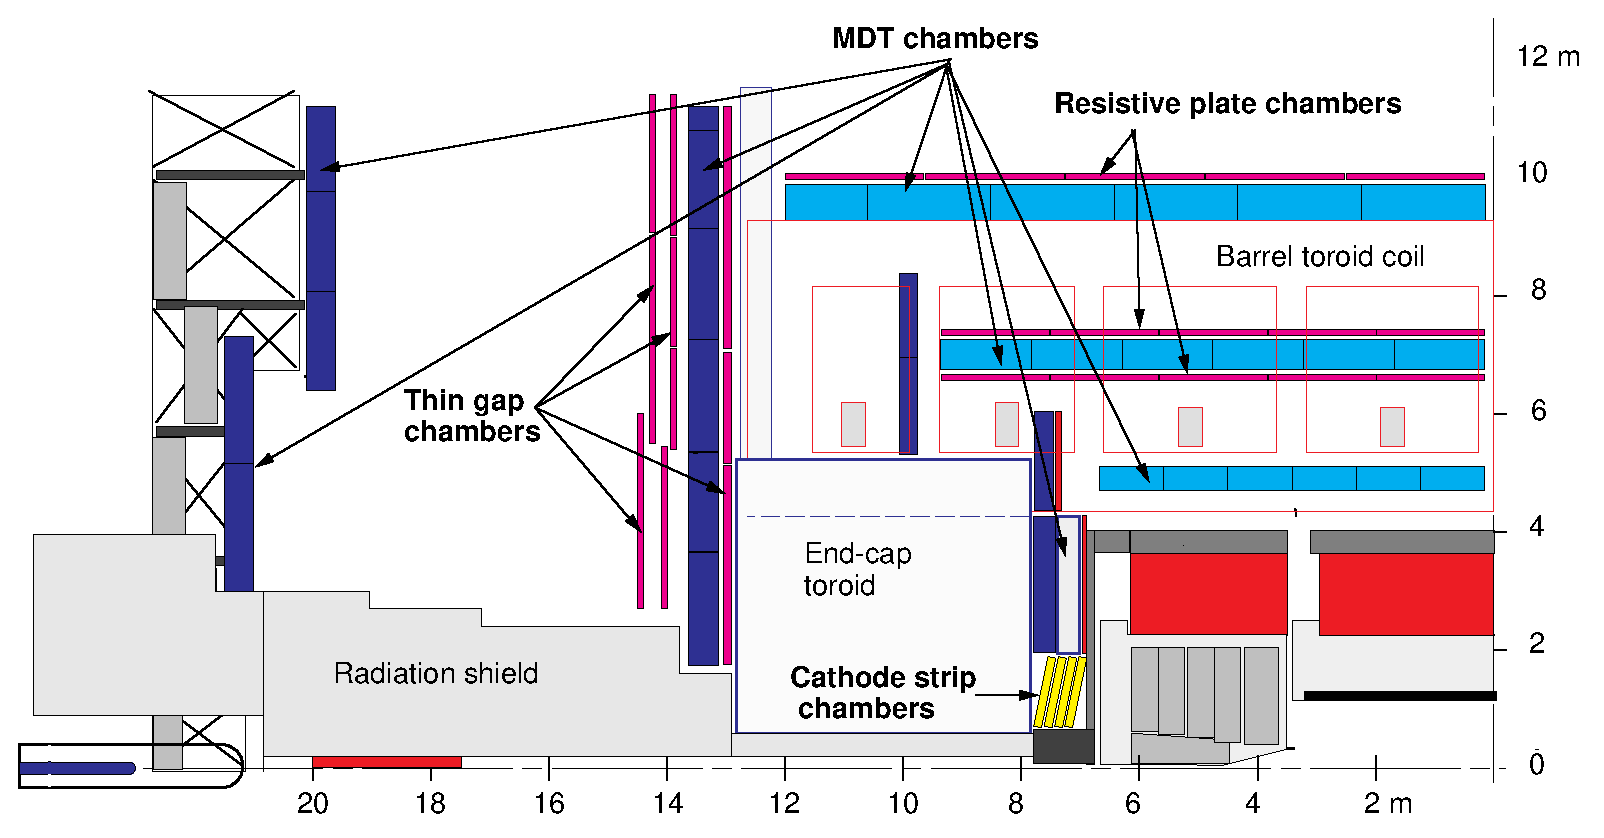
\includegraphics[width=.45\textwidth,keepaspectratio=true]{chapters/chapter2_experiment/images/ATLAS-muon-rz-tdr.eps}} \\
	% \subfloat[\label{fig:muon-spec_c}]{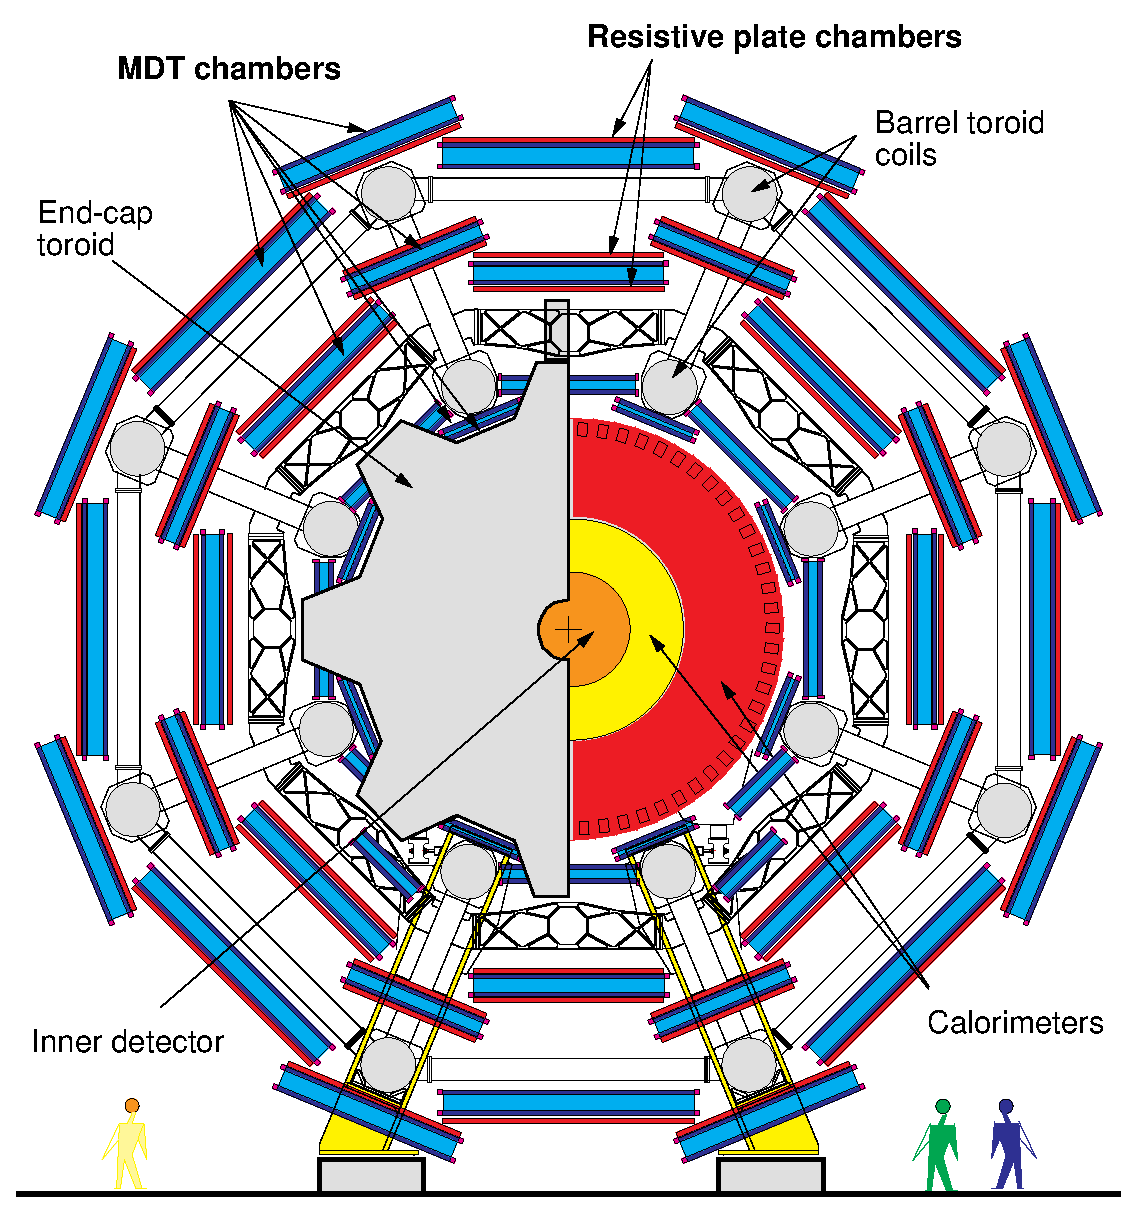
\includegraphics[width=.45\textwidth,keepaspectratio=true]{chapters/chapter2_experiment/images/ATLAS-muon-xy-tdr.eps}}
	% \caption{\label{fig:muon-spec} (a)   (b)}
	% \end{figure}

	\begin{figure}[!ht]
	\centering
	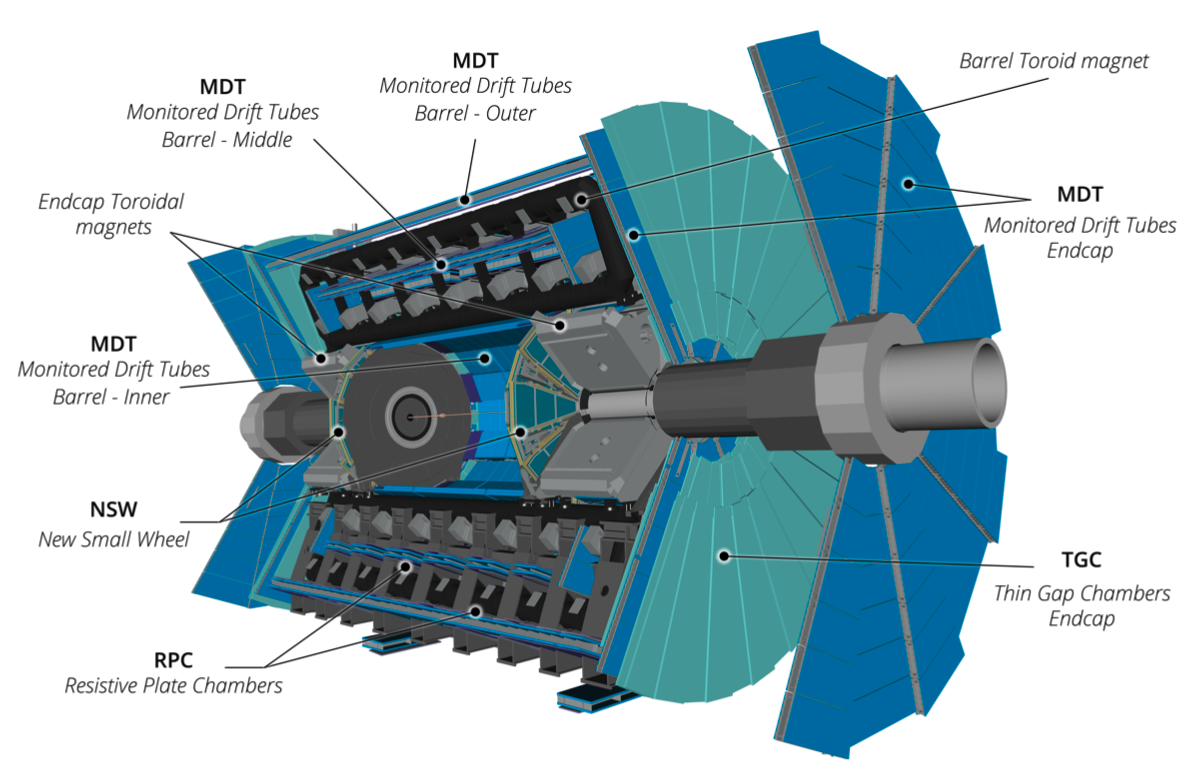
\includegraphics[width=\textwidth,keepaspectratio=true]{chapters/chapter2_experiment/images/ATLAS_Muon_System_Run3.png}
	\caption{Cut-out view of the ATLAS detector Muon Spectrometer.}
	\label{fig:muon-spec}
	\end{figure}

	\subsection{Trigger System}\label{ssec:trigger}
	The high luminosity provided by the LHC is critical in collecting enough data to make detailed physics analyses. However, it also means that there is an incredibly large amount of data to sort through. So much that it is not possible to write out the data from every bunch crossing. As shown in Figure \ref{fig:high-pileup-event-display}, even one single event can contain an inordinate amount of data. Another issue arises due to the nature of hadron collisions; in that not all bunch crossing provide hard scatter inelastic collisions that are ``interesting'' enough to save data on. 

	To solve this issue, the data coming out of ATLAS is combed through in real time at a variable rate of 1 kHz to 40 MHz. This is done with a Trigger and Data Acquisition (TDAQ) system. The TDAQ system used in Run-2 is described in detail here: \cite{ATLAS-trigger-Run2}. The TDAQ system reads in data from the ATLAS detector, calculates relevant quantities, and makes a decision on if there was an event worth storing. A diagram showing the data flow into the TDAQ system is show in \ref{fig:trigger-run2}.\footnote{Figure \ref{fig:trigger-run2} shows the Fast TracKer (FTK). During Run 2 FTK was undergoing commissioning and was not used in the active TDAQ system.} 
	\begin{figure}[!ht]
	\centering
	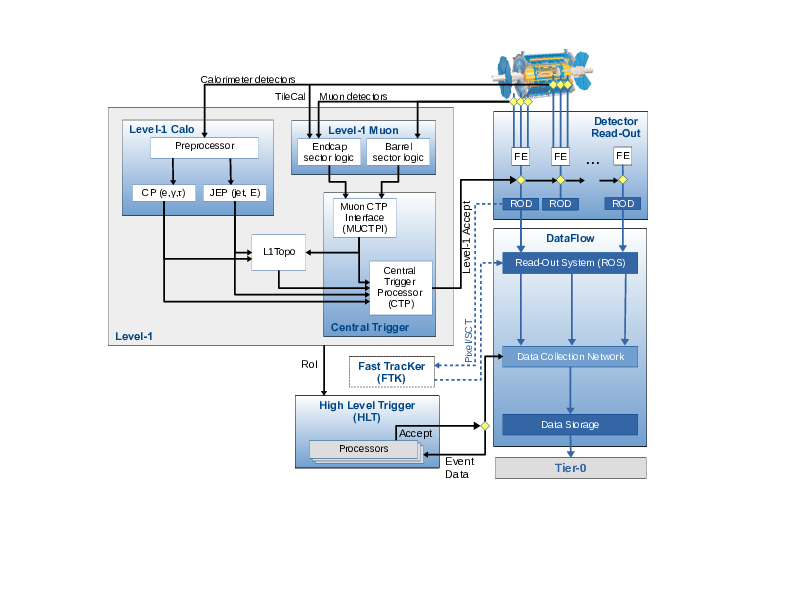
\includegraphics[width=\textwidth,keepaspectratio=true]{chapters/chapter2_experiment/images/Trigger_Run2.png}
	\caption{The ATLAS TDAQ system in Run-2 showing the components relevant for triggering as well as the detector read-out and data flow.}
	\label{fig:trigger-run2}
	\end{figure}
	The ATLAS TDAQ system consists of two main components, Level-1 (L1) and High Level Trigger (HLT). The L1 trigger is a hardware based trigger system that reads in data from the calorimeters and muon spectrometer. The L1 trigger has a latency of $2.5 \, \mu \mathrm{s}$ and can read-out accepted events up to 100 kHz, the detector maximum readout rate. The HLT is a software based trigger system based on the offline reconstruction software. During Run-2 the HLT operated with an average output rate of 1.2 kHz, which translates to about 1.2 GB/s of data sent to permanent storage.	

	After the TDAQ system accepts an event, the data is set to be stored on magnetic tape for long term storage. It is also processed at the local computing farm named Tier-0 with the full reconstruction software suite described in Chapter \ref{chap:reco}.

		% file with Chapter 2 contents
\chapter{Event Simulation and Reconstruction}

\section{Simulation} \label{sec:simulation}

To properly understand and interpret results, comparisons to theoretical prediction must be made. In the context of particle colliders, this means an understanding of both the underlying process as well as predictions of detector effects. To do this, a simulation framework has been developed by ATLAS. 

This simulation framework relies on several steps of \gls{MC} integration. A \gls{MC} simulation attempts to model a process by taking a function's underlying probability distribution and sampling it randomly. Furthermore, these steps of \gls{MC} integration evolve serially, and each step is Markovian: the process is completely dependent \textit{only} on the prior step, so sampling is performed on its posterior distribution. Producing \gls{MC} from a set of subsequent Markovian processes is known as \gls{MCMC}, which is used to simulate complex processes, such as particle collisions.

The framework is designed to produce \gls{MCMC}, evolving in steps of event generation (Section \ref{ssec:eventgen}), those events then undergo parton showering (Section \ref{ssec:partonshower}), hadronization (Section \ref{ssec:hadronization}), detector simulation (Section \ref{ssec:simulation}), and finally reconstruction of physics objects (Section \ref{sec:reconstruction}).

\subsection{Event Generation} \label{ssec:eventgen}
The first step of the ATLAS simulation is generating the hard-scatter process. At in $pp$ collisions, the object ultimately collided are partons, the constituent strongly interacting particles (quarks and gluons) that comprise the protons. When simulating collisions, parton distribution functions are used, which describe the probability of finding a parton carrying a given fraction of the proton momentum.


Event generators produce \textit{matrix elements}, which take into account the partonic cross-section to a specified order approximation. The matrix element is returned in the \textit{Les Houches Accord} format \cite{les-houches}, which was designed to create a uniform event generator output. This format can then be interfaced to tools for parton shower and hadronization.

The ATLAS software contains many event generators. For the samples used in the presented analysis, the following generators are used:

\begin{description}
    \item \HERWIGpp: A general-purpose event generator \cite{herwigpp}
    \item \MADGRAPH: A matrix element generator, generating tree-level matrix elements for Lagrangian-based models \cite{mg5}
    \item \PYTHIA: A standard event generator \cite{pythia8.2}
    \item \POWHEG: A \gls{NLO} event generator that is built to overcome the problem of negatively weighted events \cite{powheg} % Used for vbf resonant samples, check if used otherwise
    \item \SHERPA: A general-purpose simulation tool, containing all necessary components for a factorized description of scattering events \cite{sherpa2.2}
\end{description}

\subsection{Parton Showering} \label{ssec:partonshower} % https://arxiv.org/pdf/1411.4085.pdf
After interacting, the parton showering must then be simulated. As a hard scatter process accelerates, it emits \gls{QCD} bremsstrahlung radiation in the form of gluons. Emitted gluons carry color charge, which also can further radiate. This process is known as parton showering, and generators approximate these higher-order \gls{QCD} corrections through a chain of one-to-two parton branching. This is performed iteratively until reaching the non-perturbative regime, around $\unit{1}{\GeV}$.

This radiation then must be matched to the matrix element, which is done through either matching or merging. Matching uses the difference of the parton shower at fixed-order and higher-order calculation. Merging, by contrast, performs a tree-level on each parton, using resolution cuts to regulate divergences of the hard matrix element, then removes double-counting through shower branching vetoes.

Three event generators in the ATLAS software have parton shower built in: \PYTHIA, \HERWIG, and \SHERPA. Those which do not interface with one of those three for parton showering and hadronization. \PYTHIA and \SHERPA orders showers by $p_{T}$, while \HERWIG utilizes angular ordering, to account for coherence effects. 

In addition to the hard scatter process, these generators simulate the underlying event. This process accounts for effects due to rescattering or multiple parton interactions within the colliding protons.

\subsection{Hadronization} \label{ssec:hadronization}
Once partons have reached sufficiently low energies, they form hadrons. This is known as hadronization\footnote{Also known as jet fragmentation}. Hadronization is a non-perturbative process, that relies on phenomenological models alone, and those are then tuned on data. Commonly used models are the Lund string model \cite{lund-string} (\PYTHIA) or clustering models \cite{clustering-hadronization} (\HERWIG, \SHERPA).

Through hadronization, simulation is agnostic of detector, describing just the particle interaction. A schematic of the evolution of a simulated event from event generation through hadronization is shown in Figure \ref{fig:parton-shower-sketch}.

\begin{figure}[!thp]
    \centering
    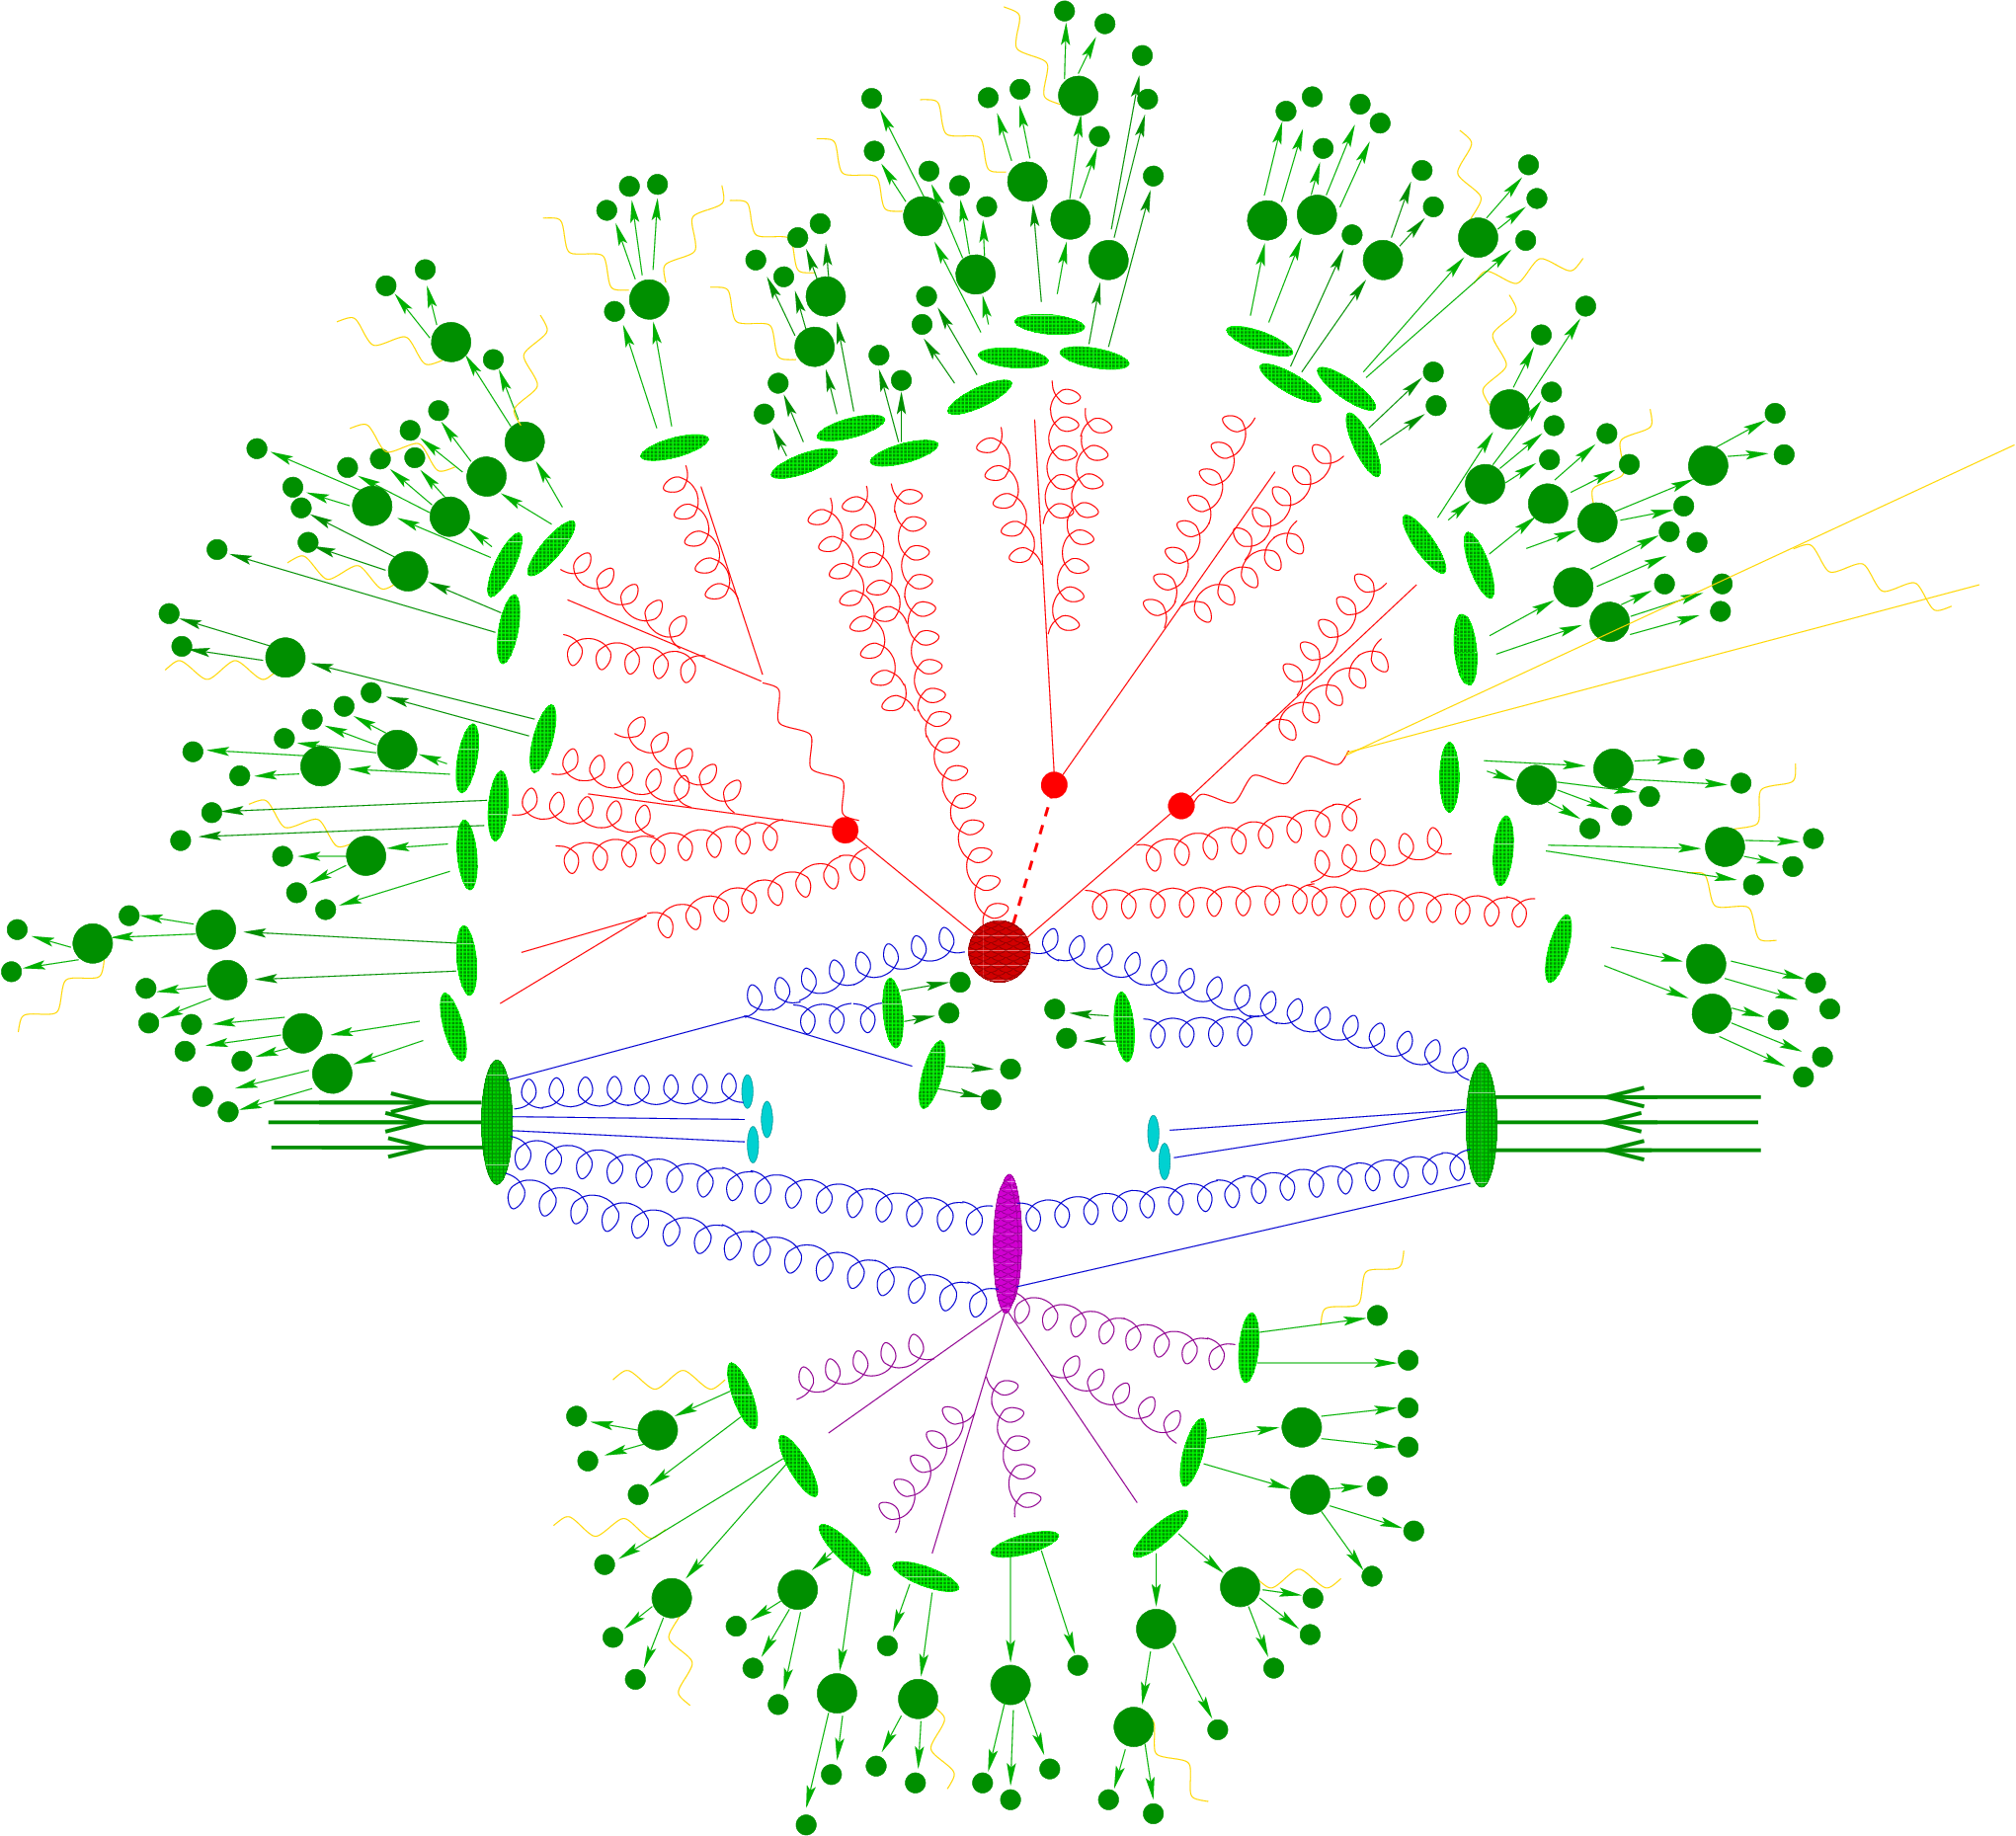
\includegraphics[width=.70\textwidth]{chapters/chapter3_eventreco/images/parton-shower.png}

    \caption[Schematic of the procession of a simulated hadron-hadron collision.]{Schematic of the procession of a simulated hadron-hadron collision through hadronization. The red circle represents the matrix element, simulated by an event generator. The emitted red lines represent the Bremsstrahlung radiation, which is simulated by a parton shower. The purple oval represents a secondary vertex. Hadronization is represented by the light green circles, in which hadrons are produced (dark green) as well as photon radiation (yellow) \cite{parton-shower-sketch}.}
    \label{fig:parton-shower-sketch}
\end{figure}


\subsection{Detector Simulation}  \label{ssec:simulation}
After hadronization, the model is a full detector-independent description of a process; next the simulation must model how the particle will interact with the ATLAS detector. In order to do this, a component-level model of the ATLAS detector is implemented in \GEANTFOUR \cite{geant4}, and particles are propagated through this model. Along the trajectory of the particle, the energy deposition in each component is calculated stochastically, and this is output as a collection of hits, and the electrical response along hits in each detector component is simulated. The output format matches that from actual data collection, so physics objects may be reconstructed via the same methods as real data, outlined in Section \ref{sec:reconstruction}.

The ATLAS simulation framework is known as \ATHENA, and is built on the Gaudi Architecture \cite{gaudi}.

\section{Object Reconstruction} \label{sec:reconstruction}

After the full simulation chain, the output is a set of hits in the ATLAS detector. Reconstruction is the method by which these hits are defined into final physics objects useful for analysis. This is performed independently for each type of signature. The following sections discuss the reconstruction of objects used in the presented analysis. For the Higgs decays, the final state physics objects are a pair of photons (discussed in \ref{ssec:em-signatures}) and a pair of jets (discussed in \ref{ssec:jet-reco}). To account for energy losses in jets, corrections using muons (discussed in \ref{ssec:muon-reco}) are applied. In addition to the objects used in this analysis, ATLAS reconstructs tau leptons and \gls{MET} (corresponding to neutrino signatures in \gls{SM} analyses, as well as a number of \gls{BSM} signatures), not discussed here.

\subsection{Electromagnetic Signatures: Electrons and Photons} \label{ssec:em-signatures} %https://arxiv.org/pdf/1908.00005.pdf

\noindent\textbf{Interaction}\\
\indent Photons and electrons interact with the \gls{LAr} calorimeter, leaving an electromagnetic signature in a group of neighboring cells known as \textit{showering}. Their reconstruction is performed in parallel due to the similarity in signature.

There are three sources that \gls{EM} clusters:
\begin{itemize}
    \item Electrons: Being a charged lepton, in addition to the showering, electrons interact with the \gls{ID}, leaving a track that can be extrapolated to the \gls{EM} cluster.
    \item Converted Photons: Photons that pair produce electron-positron pairs in the detector prior to the calorimeter have a \gls{EM} cluster matched to a secondary vertex. At low \abseta, about 20\% of photons convert, where above $\abseta=2.3$, up to 65\% convert \cite{photon-electron-perf}.
    \item Unconverted Photons: Unconverted photons do not interact with the \gls{ID}, and thus are not matched to an electron track or secondary vertex.
\end{itemize}

As a result of bremsstrahlung radiation, an electron can lose a substantial portion of its energy as it traverses the detector material. In this process, the electron radiates a photon, which itself can radiate an electron-positron pair. Should these occur in the beampipe or \gls{ID}, there may be multiple track candidates from the same electron.
%% TODO Clarify this


\noindent\textbf{Cluster Reconstruction}\\
\indent The algorithm to build electron and photon candidates is a dynamic algorithm, building variable-sized clusters known as superclusters. This is in contrast to previous methods, which use a fixed ``sliding window'' definition \cite{sliding-window}. The algorithm starts from a \textit{seed} cell, which is identified by a signal larger than a high signal threshold relative to underlying electronic noise, $S\sigma_{noise}$. The seed and its neighbors are added to the cell, known as a \textit{proto-cluster}. Then, all neighbor\footnote{In the same sampling layer, neighboring means cells are adjacent. In adjacent layers, neighboring cells must have overlap in the $(\eta,\phi)$ plane.} cells are scanned for a signal larger than a moderate threshold, $N\sigma_{noise}$. The subsequent neighbors of cells meeting this criteria are added to the cluster, and themselves evaluated if they pass the moderate signal threshold, provided that they pass a cell filter defined by $P\sigma_{noise}$. In the case where two clusters have an overlapping cell, the clusters are merged. ATLAS uses default values of $S=4,N=2,P=0$ in this algorithm. The choice of $P=0$ means that no filter is applied, and candidates passing the $2\sigma_{noise}$ have all neighboring cells added to the cluster. This method of clustering is known as  ``topological clustering'' \cite{topo-cluster}. 


The electron reconstruction efficiency is shown in Figure \ref{fig:electron-eff} as a function of truth (generator-level) \et, where this stage of candidate formation is shown in red. Due to $\unit{2.5}{\GeV}$ threshold of the clustering algorithm, the efficiency falls off below $\et = \unit{4.5}{\GeV}$.



\begin{figure}[!thp]
    \centering
    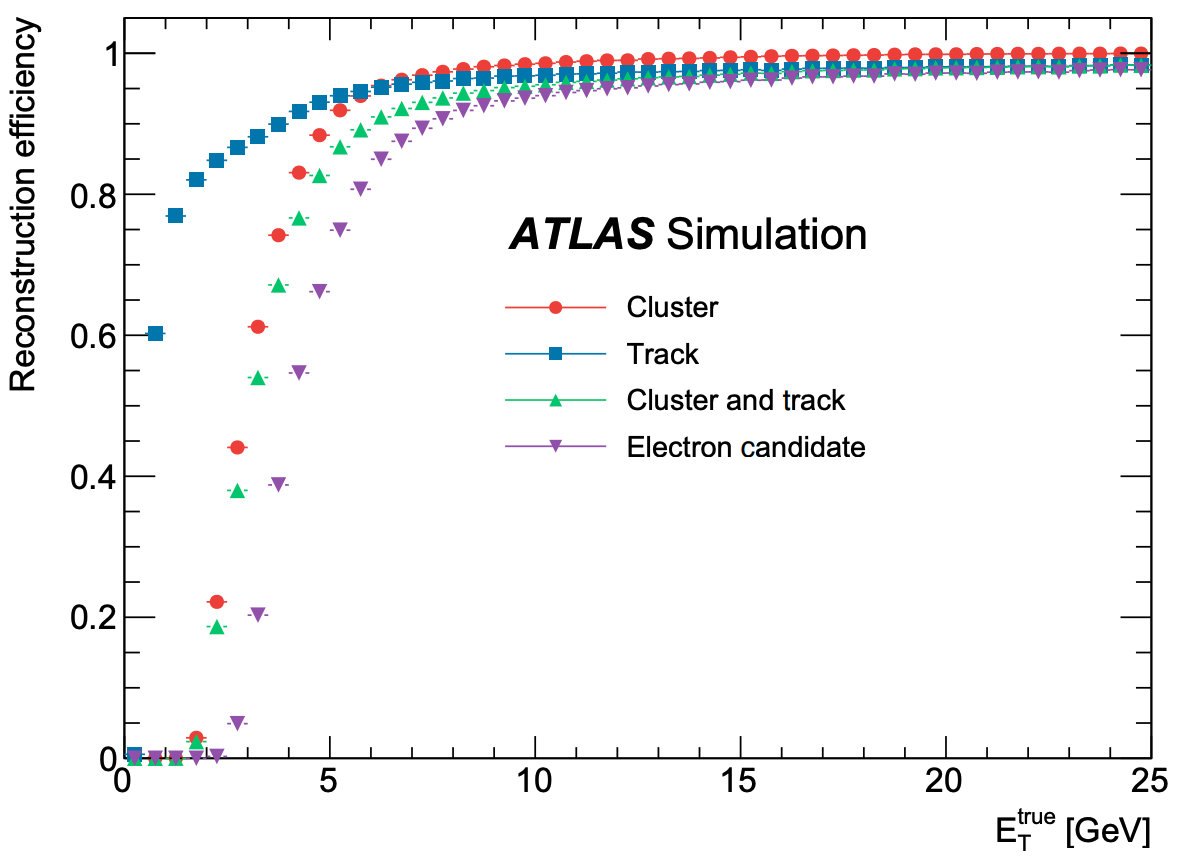
\includegraphics[width=.65\textwidth]{chapters/chapter3_eventreco/images/electron-efficiency.png}

    \caption[The reconstruction efficiency for electrons as a function of true \et.]{The reconstruction efficiency for electrons as a function of true \et for a single-electron sample. Each step of the candidate formation is shown \cite{electron-efficiency}.}
    \label{fig:electron-eff}
\end{figure}

\noindent\textbf{Track Reconstruction}\\ %https://arxiv.org/pdf/1902.04655.pdf
\indent Tracks are constructed out of hits within the \gls{ID}, in which three dimensional space-points are constructed out of clustered hits. Three sets of space-points are formed into track seeds, which then undergo stages of pattern recognition, ambiguity resolution, and \gls{TRT} extension. Track candidates with $\pt > \unit{400}{\MeV}$ are fit with the ATLAS Global $\chi^2$ fitter \cite{chi-2-fitter}. This uses the pion hypothesis for energy loss, however to accommodate for the bremsstrahlung losses, a second fit is performed using the electron hypothesis.

For tracks with at least four silicon hits that match to an \gls{EM} cluster, a secondary fit is performed using a Gaussian-sum filter \cite{gaussian-sum-filter}. This filter is is a generalization of the Kalman filter \cite{kalman-filter}, taking into account non-linearities resulting from bremsstrahlung radiation. The track perigee is then used to extrapolate to the \gls{EM} cluster in the second layer of the calorimeter, and must satisfy the following matching criteria to the cluster barycenter:
\begin{itemize}
    \item $|\eta_{cluster} - \eta_{track}| < 0.05$
    \item One of two azimuthal requirements:
    \begin{description}
        \item $-0.20 < \Delta \phi < 0.05$ for $\Delta \phi = -q \times (\phi_{cluster}-\phi_{track})$
        \item $-0.10 < \Delta \phi_{res} < 0.05$ for $\Delta \phi_{res}$ with the same definition as $\Delta \phi$,but the track momentum rescaled to the energy of the cluster
    \end{description}
\end{itemize}

%Figure \ref{fig:electron-eff} also shows the track reconstruction efficiency (blue), which is greater than 80\% efficient as low as $\et = \unit{1}{GeV}$, and more than 98\% efficient above $\et = \unit{10}{\GeV}$.




\subsection{Jets} \label{ssec:jet-reco}
As discussed in Section \ref{ssec:fermions}, strongly interacting particles cannot exist independently due to color confinement. Due to this, partons created in $pp$ collisions shower, a process where quarks radiating gluons and gluons split, ultimately creating a proliferation of subsequent partons. Ultimately, once they've reached a sufficiently low energy, about $\unit{1}{\GeV}$, they hadronize in order to create a colorless state, such as mesons or baryons that deposits energy into the calorimeters. This spray of interactions, both the showering and hadronization, all proceed in the general same direction and location, known as a ``jet.''

In principle, jets can be built from any set of 4-vector objects. For this work, they are constructed via topological clusters, described in detail in \ref{ssec:em-signatures}. Two classes of jet definitions exist. The first is cluster-based, which defines the jet by combining sets of four-vector objects until the distance between objects surpasses a stopping condition. The second is cone-based, which define jets as the sum of momenta within a defined radius, realizing jets as energy flow in a specified direction. ATLAS uses one such cone-based algorithm, known as the Anti-$k_t$ algorithm \cite{anti-kt}. The cone is built from topological clusters using a fixed radius, $R=0.4$\footnote{In analyses that probe high mass regimes, two jets may be overlapping and merge to produce one single large radius jet. This is known as a ``boosted'' topology, where the radius parameter is typically $R=1.0$. The presented analysis is not sensitive at high mass, thus such topologies are not considered.}. Since there is no a priori assumption on how fragmentation proceeds, jets are entirely defined via their algorithm.


Since all fragmenting strongly interacting particles appear as jets in the detector, an important process is \textit{flavor tagging}, which aims to classify the type of particle that produced a given jet. Paramount to the presented analysis is the process of $b$-tagging\footnote{In addition to $b$-tagging, ATLAS has also produced discriminators for charm jets ($c$-tagging).}, algorithms to classify jets which come from $b$-quarks. There are several algorithms to perform this classification, notably a \gls{BDT} named MV2 \cite{mv2-dl1} and a feed-forward deep \gls{NN}\footnote{See Appendix \ref{app:MVA} for an explanation of these multivariate techniques.} \cite{mv2-dl1}. From this score, $b$-tagging working points are established and calibrated based on their identification efficiency. 


\subsection{Muons} \label{ssec:muon-reco}
%http://cds.cern.ch/record/2139897/files/arXiv:1603.05598.pdf

Muons are a minimum-ionizing particle, leaving very little energy in the calorimeter, and are not stopped by any of the material in ATLAS. Thus, muons are reconstructed using a combination of track-based information from the \gls{ID} and the \gls{MS}. In the \gls{ID} tracks for muons is identical to other charged particles, outlined in Section \ref{ssec:em-signatures}. In the \gls{MS}, in each detector region (i.e. \glspl{MDT}, \glspl{CSC}, etc.), track segments are built from aligned hits in the bending plane of the detector, found via a Hough transform \cite{hough-transf}. Track candidates are formed by fitting together hits from different track segments via a combinatorial search outlined in Reference \cite{muon-reco}. Then an overlap removal algorithm finds the optimum track assignment. Ultimately hits are fitted with a global $\chi^2$ fit. Afterwards a hit recovery and subsequent track refit are performed if necessary.

Ultimately four muon types are defined \cite{muon-reco}:
\begin{itemize}
    \item Combined (CB) muon: Tracks reconstructed in the \gls{ID} are formed into a combined track using a global refit incorporating hits from both subdetectors.
    \item Segment-tagged (ST) muon: An \gls{ID} track is extrapolated to a local track segment in the \gls{MDT} or \gls{CSC}, accounting for muons that only cross one layer of \gls{MS} chambers.
    \item Calorimeter-tagged (CT) muon: An \gls{ID} track matched to a energy deposit in the calorimeter compatible with a minimum-ionizing particle. This muon type compensates for portions of the \gls{MS} that are only partially instrumented, near $\abseta \approx 0$.
    \item Extrapolated (ME) muons: These use only track information from the \gls{MS}, where parameters must be loosely in agreement with the location of the \gls{IP}. ME muons are useful for acceptance in $2.5 < \abseta < 2.7$, which is uncovered by the \gls{ID}.
\end{itemize}


From these muons, four selections are created (\textit{Loose}, \textit{Medium}, \textit{Tight}, and \textit{High-\pt}). These are defined based on varying requirements on the type of muon considered, number of hits, $\chi^2$ fit, $\eta$, $q/p$ \textit{significance}, and \pt. The efficiencies for the \textit{Loose} and \textit{Medium} selections are $>98\%$, and the \textit{Tight} selection ranges from $90\%$ to $98\%$ efficient. Figure \ref{fig:muon-eff} shows these efficiencies as a function of $\eta$.


\begin{figure}[!thp]
    \centering
    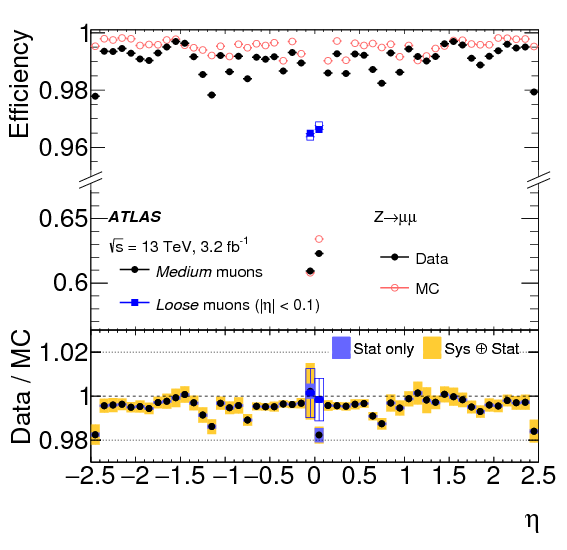
\includegraphics[width=.48\textwidth]{chapters/chapter3_eventreco/images/muon-medium.png}
    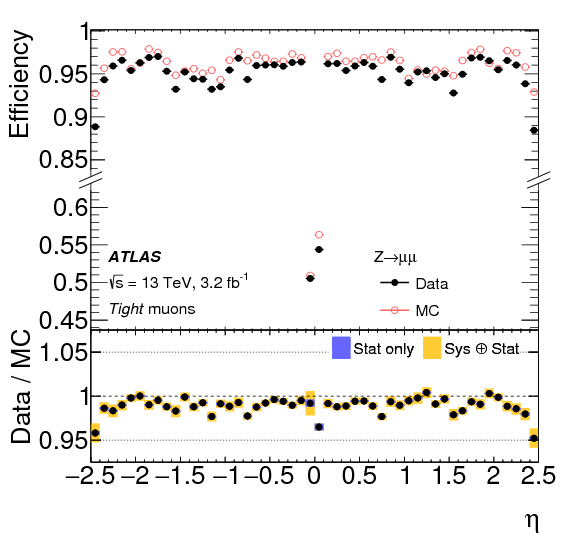
\includegraphics[width=.48\textwidth]{chapters/chapter3_eventreco/images/muon-tight.png}

    \caption[The reconstruction efficiency for \textit{Loose} and \textit{Tight} muons with $\pt >\unit{10}{\GeV}$ as a function of $\eta$.]
    {The reconstruction efficiency for muons with $\pt >\unit{10}{\GeV}$ as a function of $\eta$. The left panel shows the \textit{Loose} selection, the right shows the \textit{Tight} selection \cite{muon-reco}.}
    \label{fig:muon-eff}
\end{figure}
		
\chapter{Photon Identification Optimization}

Photon identification in ATLAS is carried out through applying cuts to 9 shower shape variables that explain the longitudinal and lateral showering development of electromagnetic interaction in the calorimeter. These include variables describing the leakage in the hadronic calorimeter ($R_{had}$, $R_{had_1}$), widths of energy depositions in the \gls{EM} calorimeter ($w_{\eta_2}$, $w_{s3}$), energy ratios of depositions in the \gls{EM} calorimeter ($R_{\eta}$, $R_{\phi}$, $F_{side}$), and the energy difference and ratios of the strips ($\Delta E$, $E_{ratio}$). A schematic of all these variables can be found in Figure \ref{fig:ss-vars-schematic}. Additionally, a table describing these variables can be found in Table \ref{tab:ss-vars-table}. Two sets of cuts are defined, corresponding to two working points, nominally the \textit{tight} and \textit{loose} menus.

\begin{figure}
    \centering
    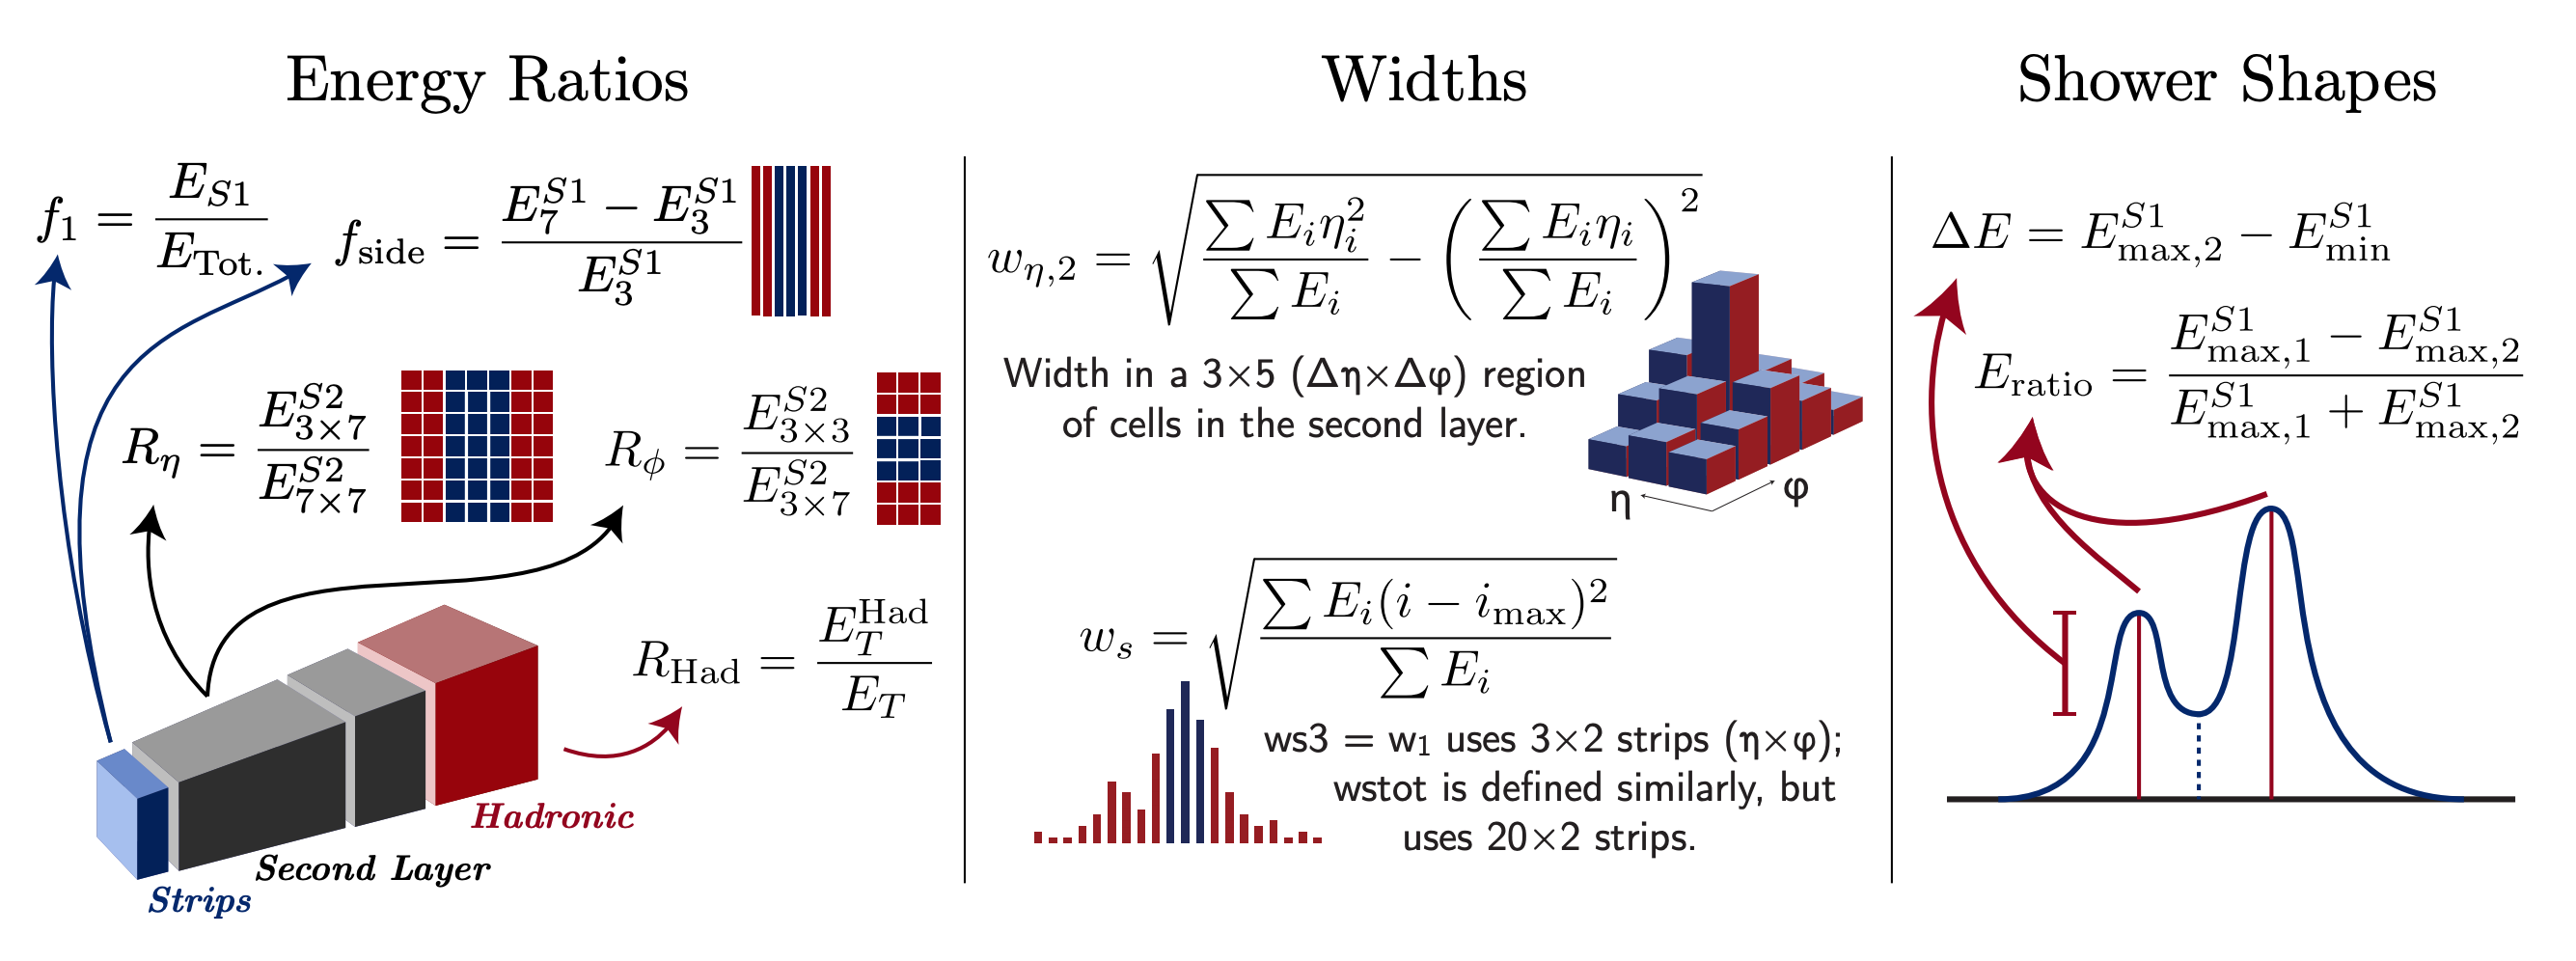
\includegraphics[width=.98\textwidth]{chapters/chapter4_photonID/images/ss-vars.png}
    \caption[Schematic of the shower shape variables used in the present cut-based photon identification menu.]
    {Schematic of the shower shape variables used in the present cut-based photon identification menu \cite{ss-var-schematic}.}
    \label{fig:ss-vars-schematic}
\end{figure}

\begin{table}
    \centering
    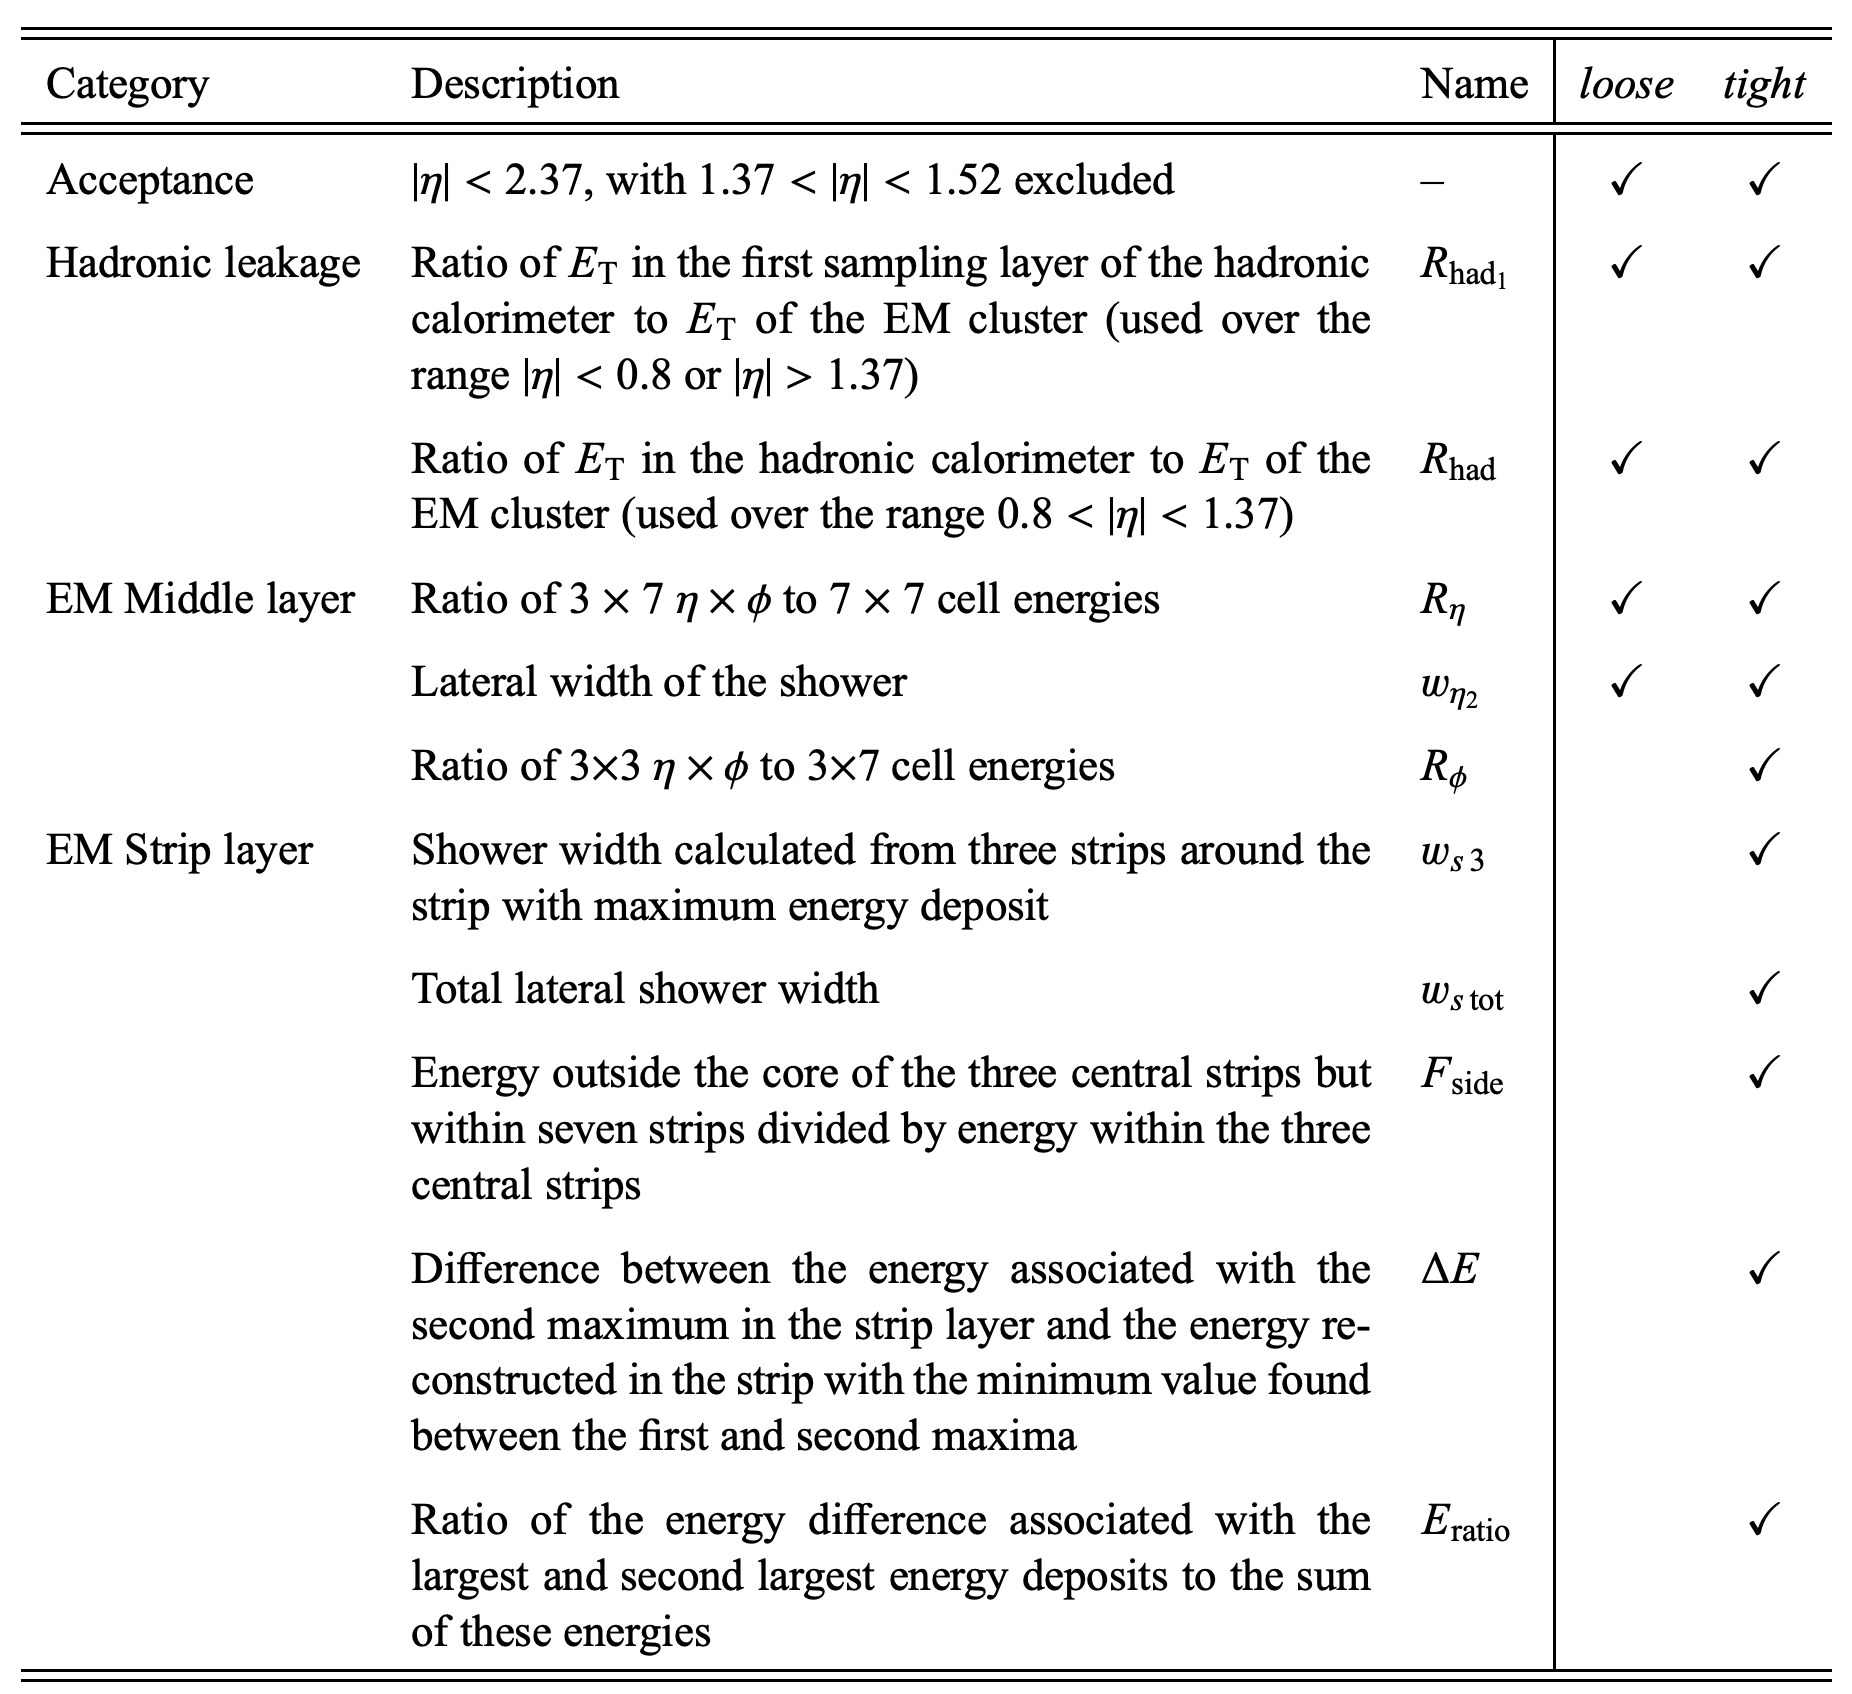
\includegraphics[width=.90\textwidth]{chapters/chapter4_photonID/images/ss-table.png}
    \caption[List of discriminating variables used in the present photon identification menu.]
    {List of discriminating variables used in the present photon identification menu \cite{r1-photonID}.}
    \label{tab:ss-vars-table}
\end{table}

% todo: maybe describe these a bit better https://arxiv.org/pdf/1606.01813.pdf 

In order to account for detector segmentation and differences in upstream material, cuts on these variables are derived in bins of \abseta. The intervals are 0.0, 0.6, 0.8, 1.15, 1.37, 1.52, 1.81, 2.01, 2.37, with a bin defined between each step (e.g. $[0.0,0.6)$, $[0.6,0.8)$, etc.) except over $[1.37,1.52)$ where the transition crack between the \gls{EMB} and \gls{EMEC} lies. 

% TODO : pT binning

\section{Samples} \label{sec:photon-id-samples}

In optimization of photon identification, the aim is to discriminate prompt photons from various background sources. The predominant background is that from hadronically decaying jets. 

For these studies, a sample of leading-order $\gamma+$jet events from $qg \rightarrow q \gamma$ and $q\bar{q} \rightarrow g \gamma$ hard scattering, as well as and quark fragmentation in QCD dijet events is used. Additionally, \gls{MC} truth information is used to require a prompt photon in the event. For background, a sample of all tree-level $2\rightarrow2$ QCD processes, except $\gamma+$jet events from quark fragmentation is used. \gls{MC} truth information is used to veto prompt photons in this sample as well. Both samples are generated using \PYTHIA. For both samples, simulation matched the detector conditions in the 2015 and 2016 data taking period. 



\section{Topological Clusters}

Photon reconstruction is performed through a method known as ``topological clustering,'' which is outlined in Section \ref{ssec:em-signatures}. In the calorimeter, energy depositions are clustered via this method, then merged into superclusters, which are ultimately the detector signature defined as the photon. The reconstructed observables of these topological clusters, or \textit{moments}, can be used to characterize them. This section will discuss the use of these topological cluster moments in photon identification to better reject background from non-prompt photons.

\noindent\textbf{Number of Topo-Clusters}\\
\indent As described in Section \ref{ssec:em-signatures}, photons are  superclusters, which can be made up of one or more topo-clusters as a result of cluster splitting or bremsstrahlung radiation. In over 90\% of photon events, there is only 1 topo-cluster associated to the photon supercluster. As a result, the quantities studied as inputs are all of the leading topo-cluster. Additionally, the number of topo-clusters is on average fewer for prompt photons than fakes, so this value is used as an input into the photon identification menu.


\begin{figure}
    \centering
    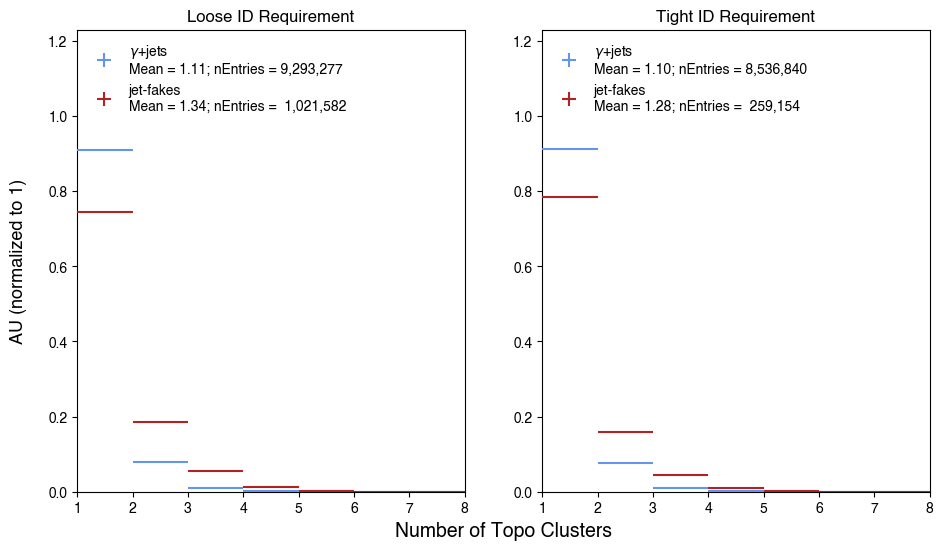
\includegraphics[width=\textwidth]{chapters/chapter4_photonID/images/hists/y_nTopoClusters.png}
    \caption[Number of topo-clusters in photon superclusters]
    {Number of topo-clusters in photon superclusters in truth-matched $\gamma+$jet events and truth-vetoed jet fake events} 
    \label{fig:topo-geom}
\end{figure}


\noindent\textbf{Shape Information}\\
\indent The size of the topological cell is parametrized by moments in $r_i$ and $\lambda_i$, which are defined as:

\begin{equation}
    r_i = |(\vec{x_i} - \vec{c}) \times \vec{s}| \text{\hspace{2em}(radial distance to shower axis)} \\
\end{equation}
\begin{equation}
    \lambda_i = (\vec{x_i} - \vec{c}) \cdot \vec{s} \text{\hspace{2em}(longitudinal distance to shower center of gravity)} 
\end{equation}

Where $\vec{s}$ is the shower axis and $\vec{c}$ is the center of gravity. Through this parametrization, the topo-cluster can be analyzed as a spheroid, with the second moments in $r$ and $\lambda$ as the extensions. $\sqrt{\langle \lambda^2 \rangle}$ is the semi-major axis in depth (along the shower axis), $\sqrt{\langle r^2 \rangle}$ is the semi-major axis in width. The distribution of these two parameters are shown for the leading topo cluster in Figures \ref{fig:topo-secondLambda} and \ref{fig:topo-secondR}, after applying the current loose and tight photon identification criteria.

\begin{figure}
    \centering
    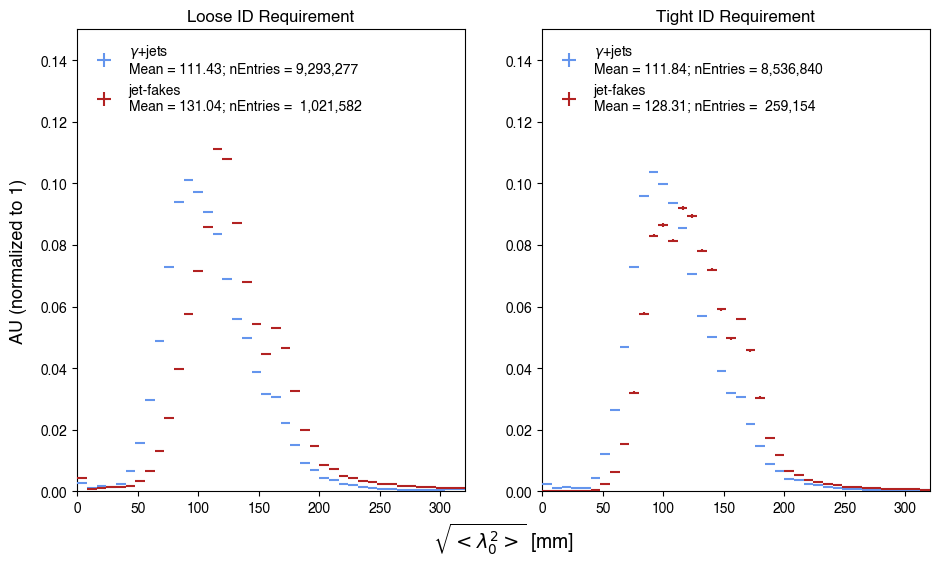
\includegraphics[width=\textwidth]{chapters/chapter4_photonID/images/hists/y_topoCluster0_secondLambda.png}
    \caption[The distribution of the semi-major axis in depth, $\sqrt{\langle \lambda^2 \rangle}$, for the leading topo-cluster]{The distribution of the semi-major axis in depth, $\sqrt{\langle \lambda^2 \rangle}$, for the leading topo-cluster in truth-matched $\gamma+$jet events and truth-vetoed jet fake events.}
    \label{fig:topo-secondLambda}

\end{figure}

\begin{figure}[t]
    \centering 
    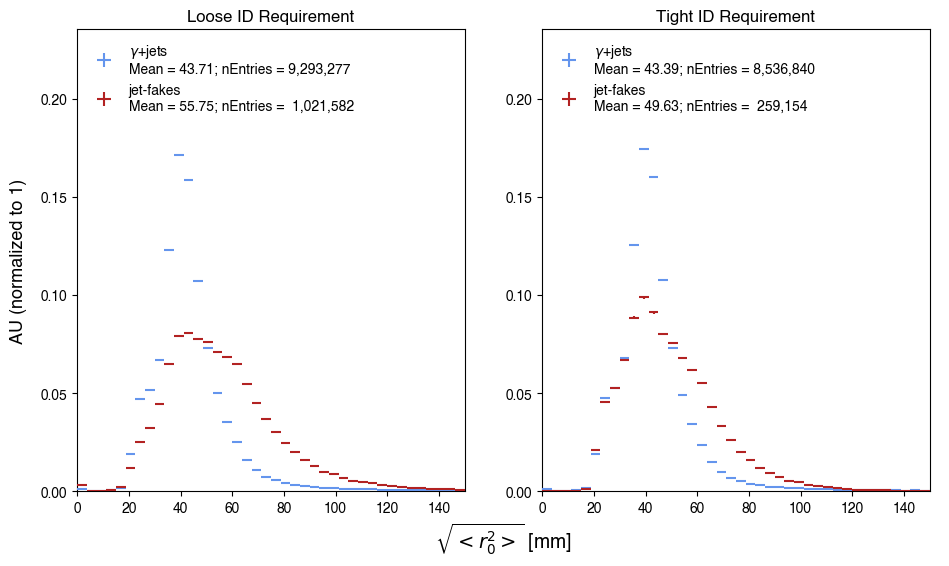
\includegraphics[width=\textwidth]{chapters/chapter4_photonID/images/hists/y_topoCluster0_secondR.png}
    \caption[The distribution of the semi-major axis in width, $\sqrt{\langle r^2 \rangle}$, for the leading topo-cluster]{The distribution of the semi-major axis in width, $\sqrt{\langle r^2 \rangle}$, for the leading topo-cluster in truth-matched $\gamma+$jet events and truth-vetoed jet fake events.}
    \label{fig:topo-secondR}
\end{figure}



\noindent\textbf{Location Information}\\
\indent The location of the topo-cluster is calculated from the first moments of the three cartesian coordinates, describing the position of $\vec{c}$. Due to azimuthal symmetry in the detector, the key component to locational parametrization of topo-clusters is the depth in the calorimeter. Thus, this location can be described via $\lambda_{clus}$, the distance of the center of gravity from the front face of the calorimeter. This distribution is shown in Figure \ref{fig:topo-centerLambda}.

\begin{figure}
    \centering 
    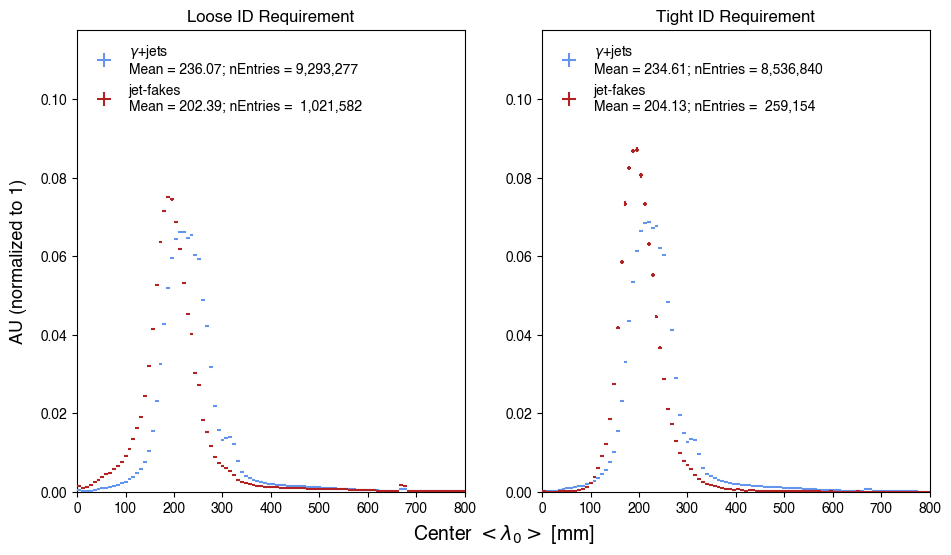
\includegraphics[width=\textwidth]{chapters/chapter4_photonID/images/hists/y_topoCluster0_centerLambda.png}
    \caption[The distribution of the centroid depth ($<\lambda_{0}>$) of the leading topo-cluster]{The distribution of the centroid depth ($<\lambda_{0}>$) of the leading topo-cluster in truth-matched $\gamma+$jet events and truth-vetoed jet fake events.}
    \label{fig:topo-centerLambda}
\end{figure}

A visualization of the geometric moments, both location and shape can be found in Figure \ref{fig:topo-geom}, with relevant spacial parameters (i.e. $\vec{c}$, $\vec{s}$, etc) shown and defined.

\begin{figure}
    \centering
    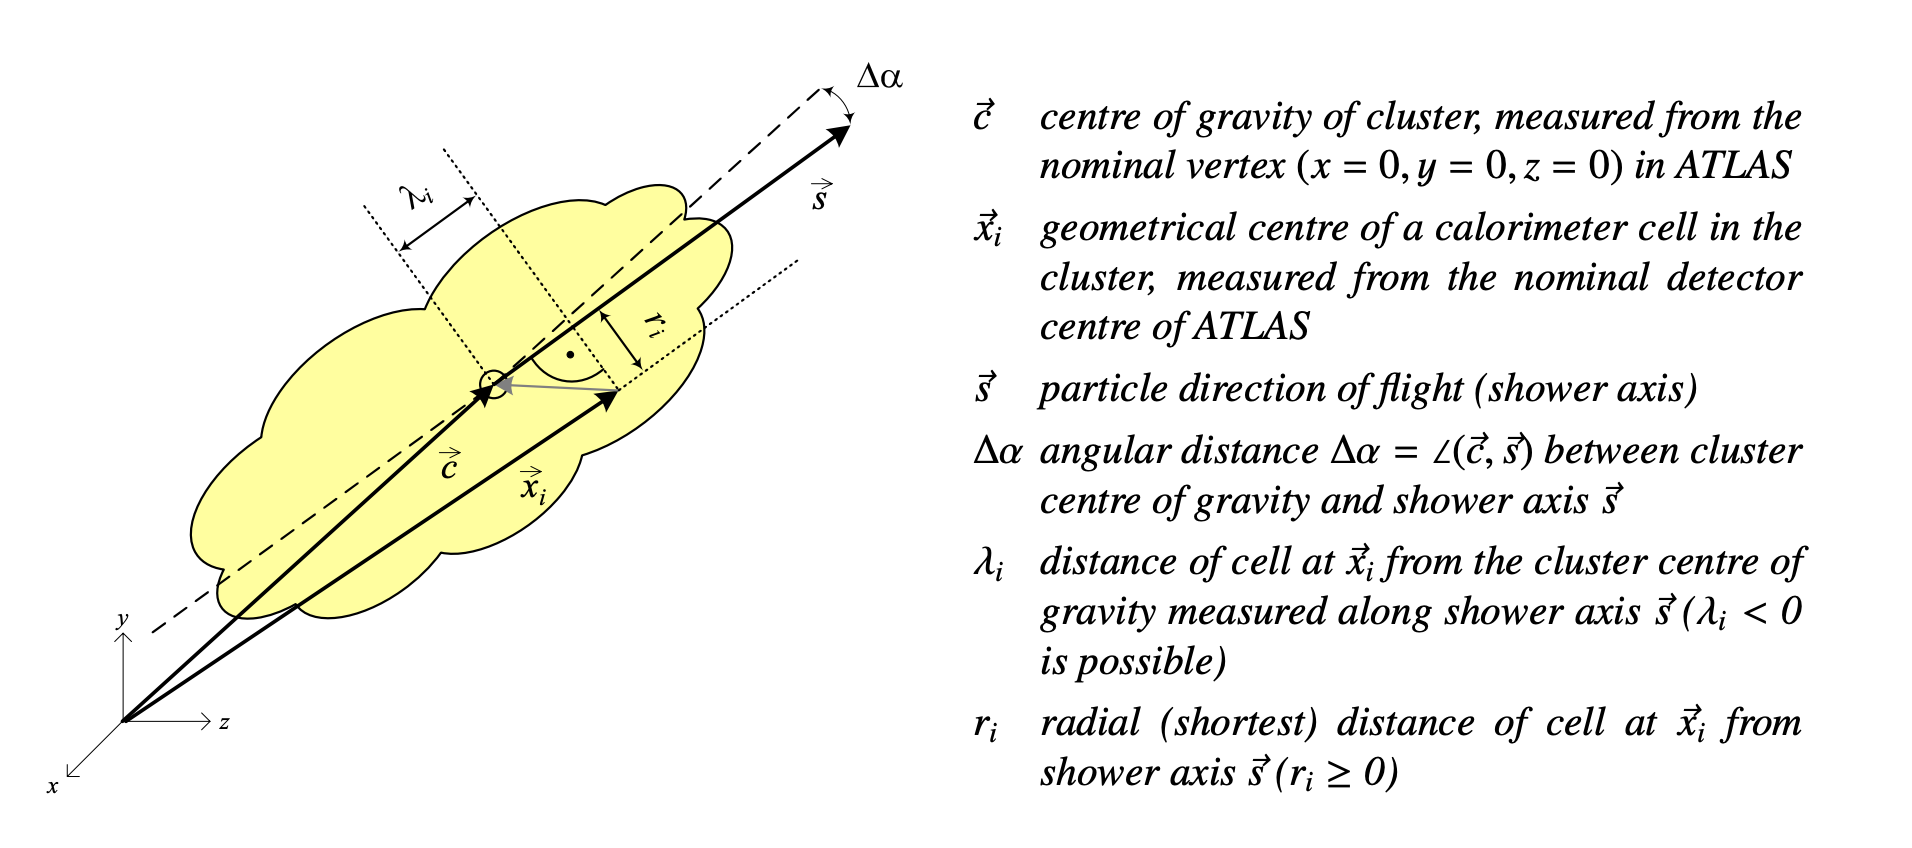
\includegraphics[width=.90\textwidth]{chapters/chapter4_photonID/images/geom-moments.png}

    \caption[The geometric moments and relevant parameters for topo-clusters.]
    {The geometric moments and relevant parameters for topo-clusters \cite{topo-clustering-r1}.}
    \label{fig:topo-geom}
\end{figure}


\noindent\textbf{Additional Moments}\\
\indent Beyond the shape and location information, there are several other moments that can be used. Two are considered as inputs into the photon identification menu, cluster isolation and \gls{EM} probability.

The signal thresholds built into the topological clustering algorithm are constructed to suppress noise, but lead to signal losses at the perimeter of clusters. The isolation moment, $f_{\text{iso}}$, measures the degree of isolation of a cluster. It is constructed as a weighted fraction of the sampling layer energy ($E_{s}^{\text{EM}}$) of non-clustered neighbor cells on the perimeter of the topo-cluster in the sampling layer. It is given by

\begin{equation}
    f_{\text{iso}} = \frac
    {
    \sum_{S \in \{ \text{samplings with} E_{s}^{\text{EM}} > 0 \} }  
    E_{s}^{\text{EM}} N_{\text{cell},s}^{\text{noclus}} / N_{\text{cell},s}^{\text{neighbor}}
    } 
    {
        \sum_{S \in \{ \text{samplings with} E_{s}^{\text{EM}} > 0 \} }
    }.
\end{equation}

Here, $N_{\text{cell},s}^{\text{noclus}} / N_{\text{cell},s}^{\text{neighbor}}$ is the ratio of unclustered perimeter cells to the total number of perimeter cells for a given cluster. This is summed across all sampling layers with positive energy, $s$. For the signal and background samples, the isolation is shown using the existing loose and tight identification criteria in Figure \ref{fig:topo-isolation}.

\begin{figure}[t]
    \centering 
    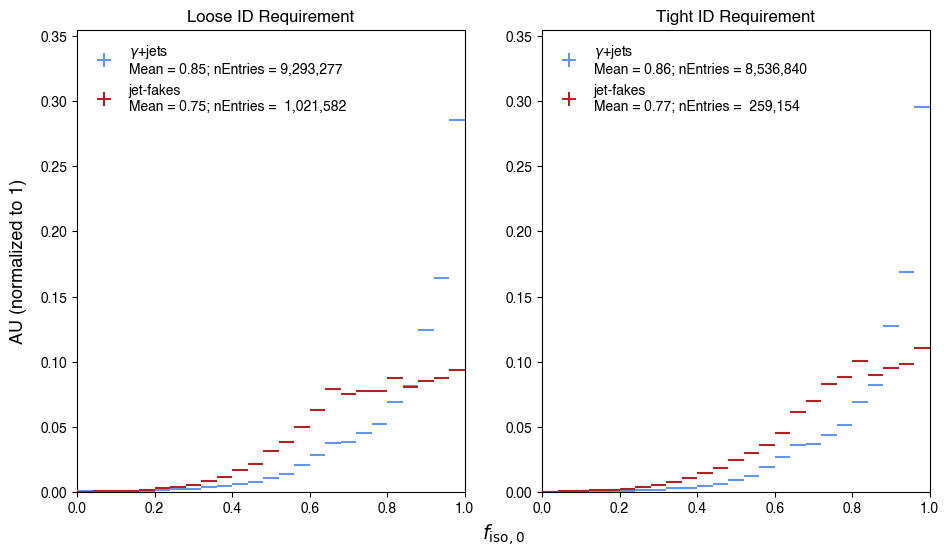
\includegraphics[width=\textwidth]{chapters/chapter4_photonID/images/hists/y_topoCluster0_isolation.png}
    \caption[The distribution of the isolation moment of the leading topo-cluster]{The distribution of the isolation moment of the leading topo-cluster in truth-matched $\gamma+$jet events and truth-vetoed jet fake events}
    \label{fig:topo-isolation}
\end{figure}

Energy losses in topo-clusters are corrected through a method known as \glsfirst{LCW} calibration. Since energy losses differ between hadronic and electromagnetic deposits, the \gls{LCW} calibration includes a step where the probability that a topo-cluster originates from an electromagnetic shower is evaluated.

The likelihood is defined through measuring the efficiency for detecting an EM-like cluster in bins of four other topo-cluster observables, defined by

\begin{equation}
    \mathfrak{O}_{\text{clus}}^{\text{class}} = \{
        E_{\text{clus}}^{\text{EM}},
        \eta_{\text{clus}},
        \log_{10}(\rho_{\text{clus}} / \rho_{\text{0}}) - \log_{10}(E_{\text{clus}}^{\text{EM}} / E_{\text{0}}),
        \log_{10}(\lambda_{\text{clus}} / \lambda_{\text{0}}
    \}
\end{equation}

where $\rho_0 = 1$ MeV mm$^-3$, $E_0 = \unit{1}{\MeV}$, $\lambda_{0} = \unit{1}{\mm}$. These bins (denoted $ijkl$) can then be used to define the likelihood, $ \mathcal{P}_{\text{clus}}^{\text{EM}}$, in each bin as


\begin{equation}
    \mathcal{P}_{\text{clus}}^{\text{EM}} ( E_{\text{clus}}^{\text{EM}}, \eta_{\text{clus}}, \rho_{\text{clus}} / E_{\text{clus}}^{\text{EM}}, \lambda_{\text{clus}}) \mapsto \mathcal{P}_{\text{clus}, ijkl}^{\text{EM}}  = \frac{\epsilon^{\pi^0}_{ijkl}}{ \epsilon^{\pi^0}_{ijkl} + 2\epsilon^{\pi^\pm}_{ijkl}}
\end{equation}


Where $\epsilon^{\pi^0(\pi^\pm)}_{ijkl}$ is the efficiency, defined as
\begin{equation}
    \epsilon^{\pi^0(\pi^\pm)}_{ijkl} = \frac{ N^{\pi^0(\pi^\pm)}_{ijkl} }{N^{\pi^0(\pi^\pm)}_{ij}}
\end{equation}

For $N^{\pi^0(\pi^\pm)}_{ijkl}$ topo-clusters in a given bin $ijkl$ and $N^{\pi^0(\pi^\pm)}_{ij}$ topo-clusters in bin $ij$ of the $(E_{\text{clus}}^{\text{EM}}, \eta_{\text{clus}})$ phase space. This likelihood, $\mathcal{P}_{\text{clus}}^{\text{EM}}$, by definition is bounded from 0 to 1, and considered as an input into the photon ID menu. This distribution is shown in Figure \ref{fig:topo-emProb}, with both the current loose and tight photon identification criteria applied.

\begin{figure}[!th]
    \centering 
    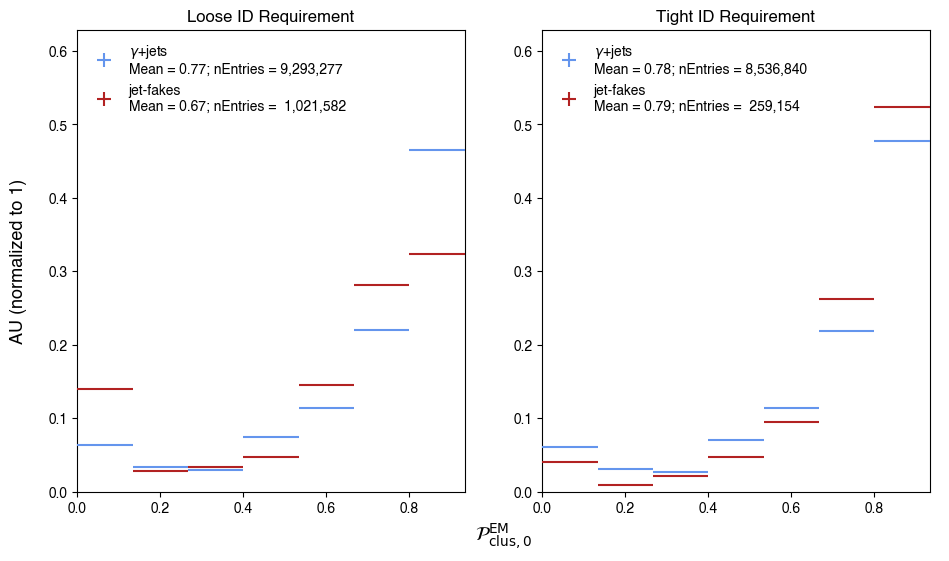
\includegraphics[width=\textwidth]{chapters/chapter4_photonID/images/hists/y_topoCluster0_emProbability.png}
    \caption[The distribution of the \gls{EM} probability moment of the leading topo-cluster]{The distribution of the \gls{EM} probability moment of the leading topo-cluster in truth-matched $\gamma+$jet events and truth-vetoed jet fake events}
    \label{fig:topo-emProb}
\end{figure}


\subsection{Data-MC Comparison}
In order to ensure that the topological clusters are properly modeled in the \gls{MC}, the variables investigated are compared to data. To do so, the present tight photon ID is applied to both the \gls{MC} and data. Furthermore, photons in \gls{MC} must correspond to a truth photon. 


This section includes the comparisons for unconverted photons which are considered for adding to the photon ID menu. Converted comparisons will be included into Appendix 

% TODO: add appendix

%todo: add plots

\begin{figure}[!thp]
    \centering
    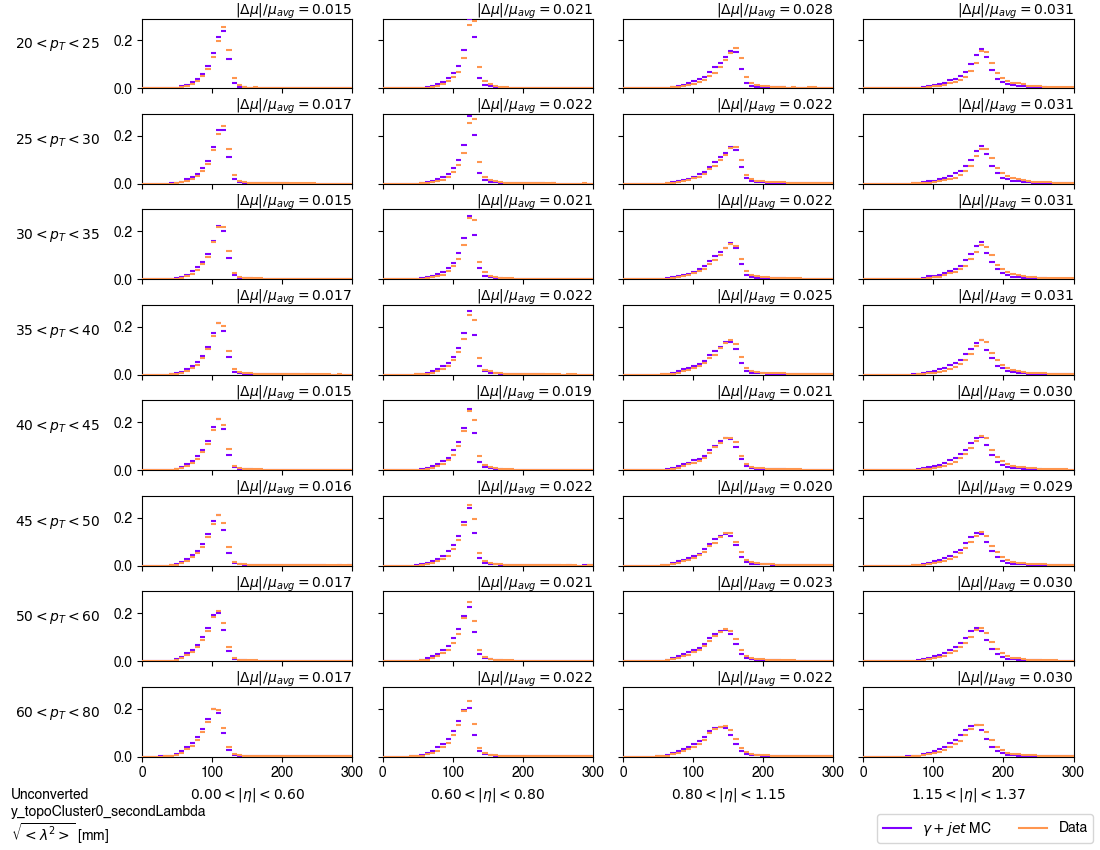
\includegraphics[width=.80\textwidth]{chapters/chapter4_photonID/images/y_topoCluster0_secondLambda_Unconverted_lowerEta.png}
    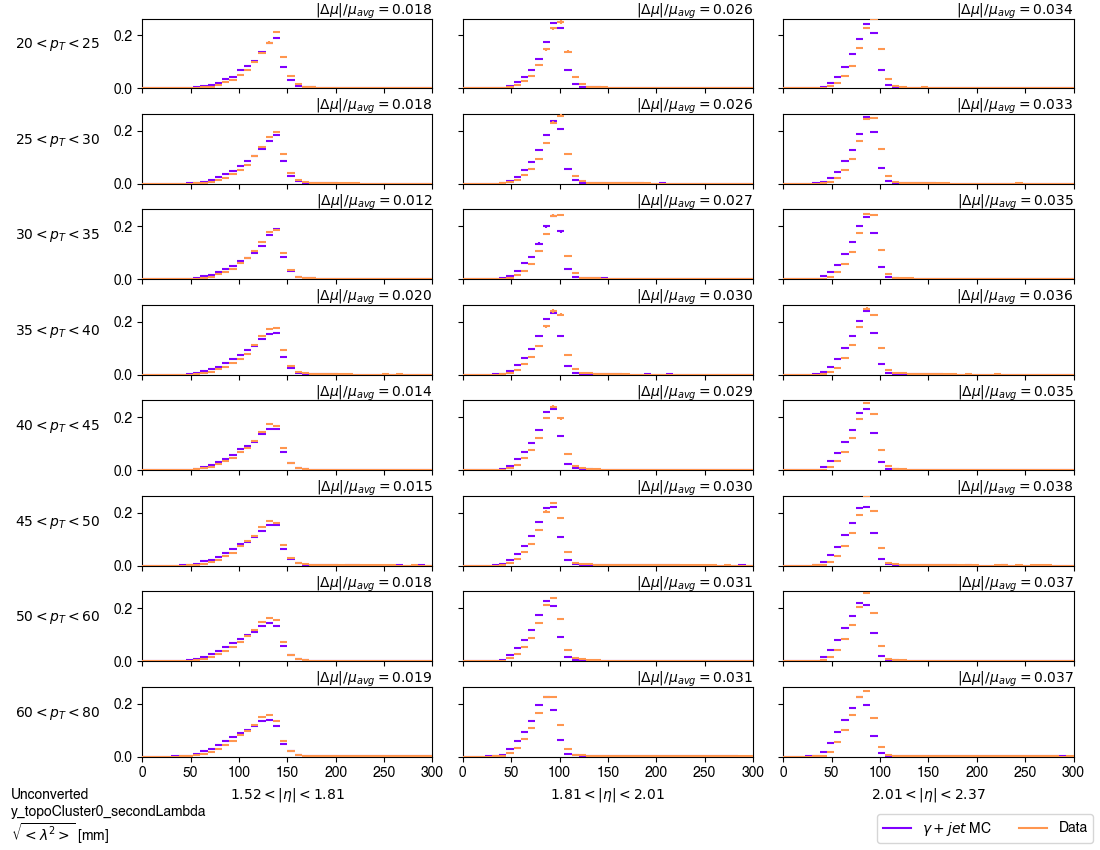
\includegraphics[width=.80\textwidth]{chapters/chapter4_photonID/images/y_topoCluster0_secondLambda_Unconverted_upperEta.png}
    \caption{Data-MC comparison for the semi-major axis in depth ($\sqrt{\lambda^2}$).}
\end{figure}
\begin{figure}[!thp]
    \centering
    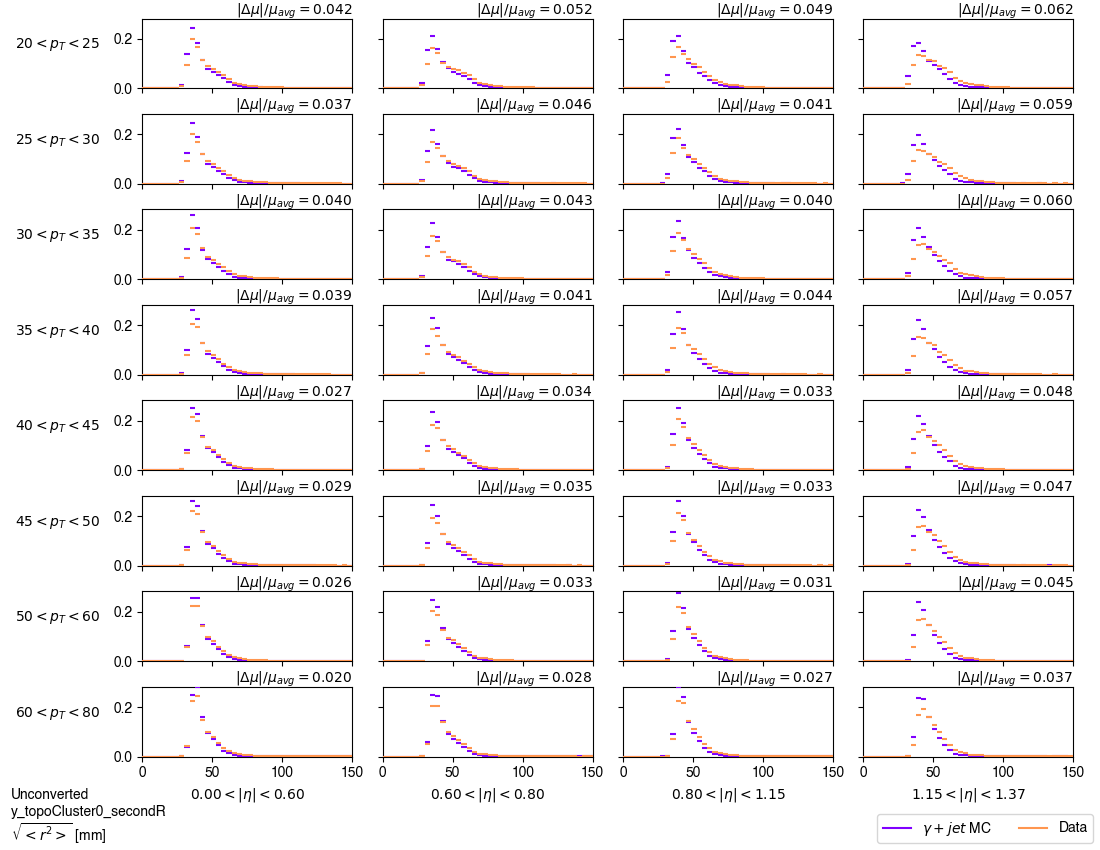
\includegraphics[width=.80\textwidth]{chapters/chapter4_photonID/images/y_topoCluster0_secondR_Unconverted_lowerEta.png}
    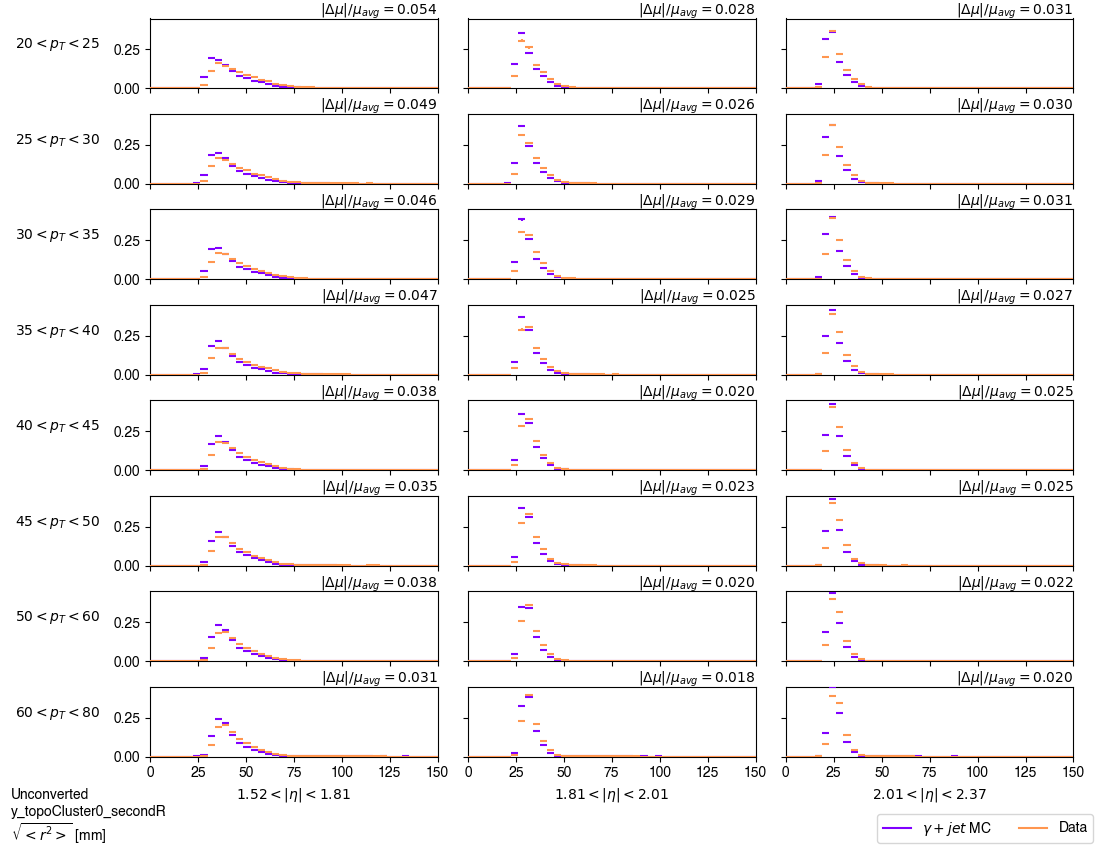
\includegraphics[width=.80\textwidth]{chapters/chapter4_photonID/images/y_topoCluster0_secondR_Unconverted_upperEta.png}
    \caption{Data-MC comparison for the semi-major axis in width ($\sqrt{r^2}$).}
\end{figure}
% TODO: split these figs?

\noindent\textbf{Correlations}\\
\indent Checking the correlations of variables is important for several reasons. First, highly correlated variables do not bring new information, and thus are not useful for adding additional cuts on. Also, it is paramount that any variables that are incorporated in the menu are not correlated to photon isolation. The correlation between these variables and the shower shape variables and isolation working points is shown in Figure \ref{fig:photonid-corrs}. 
%todo: add plots

\begin{figure}[!thp]
    \centering
    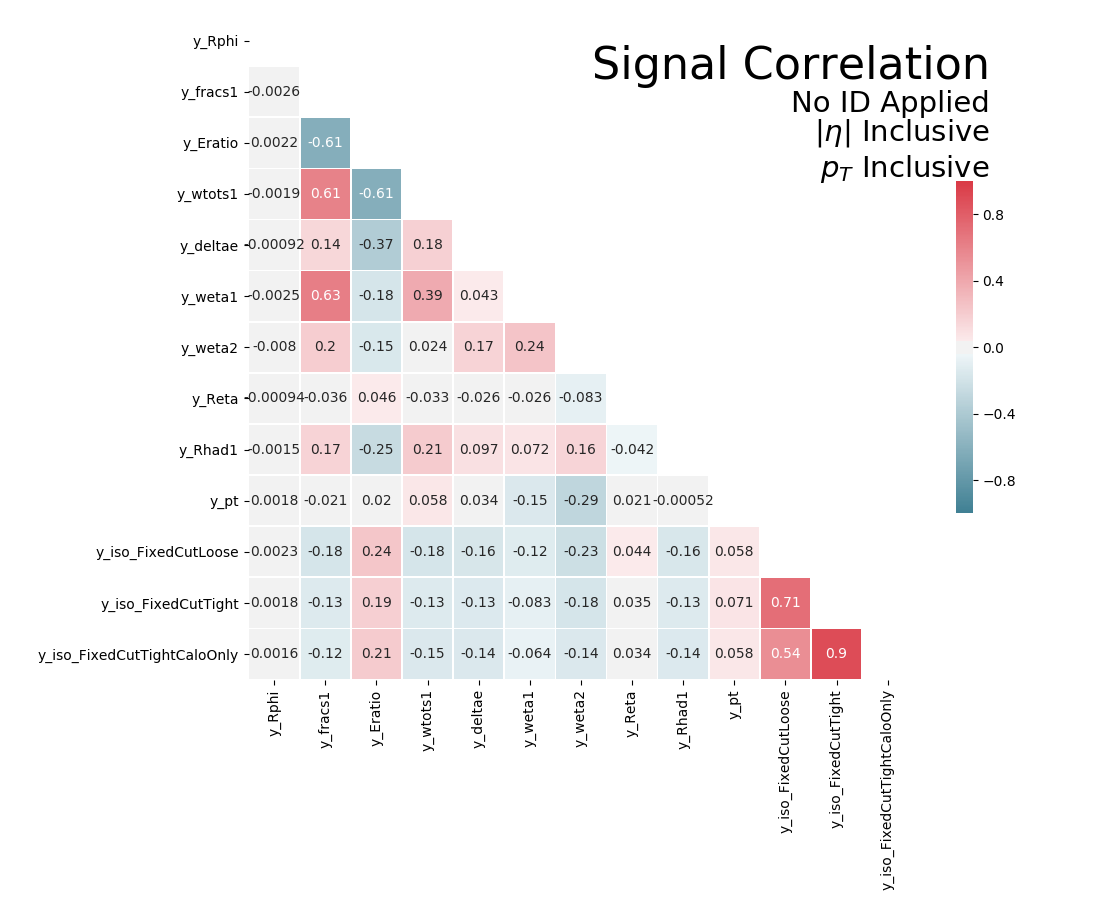
\includegraphics[width=.77\textwidth]{chapters/chapter4_photonID/images/sig_none_corr.png}
    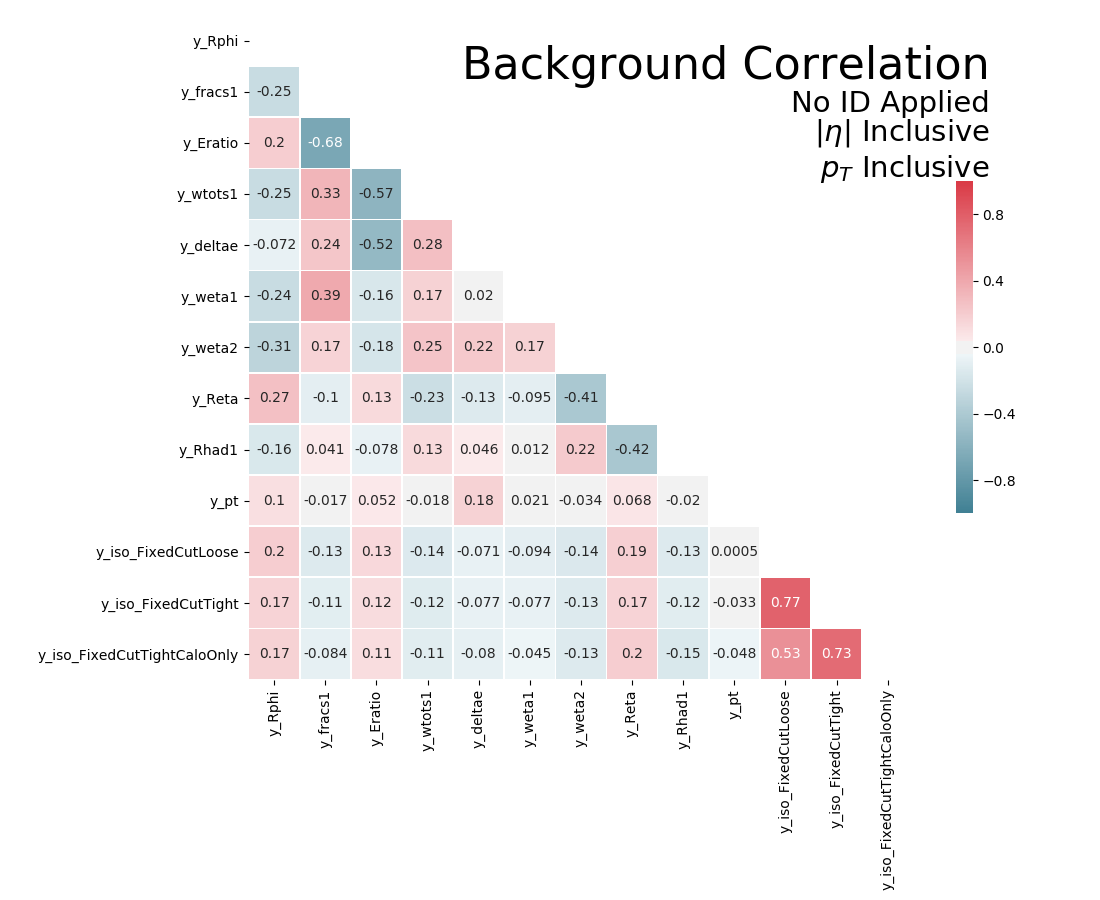
\includegraphics[width=.77\textwidth]{chapters/chapter4_photonID/images/bkg_none_corr.png}
    \caption{Correlation values between the shower shape variables, topological cluster variables, and isolation working points.}
    \label{fig:photonid-corrs}
\end{figure}
% TODO: split these figs?

\subsection{Incorporating into Menu}

The topological cluster variables were added to the existing shower shape variable-based menu. The cut-based approach is reoptimized including the new variables, and new cuts are derived in each $\eta$-\pt bin.  To compare improvement across bins, a figure of merit is defined, the improvement in background rejection for the same signal efficiency as the current photon identification menu. In formulaic terms:

\begin{align}
    Z_{\text{rel}} &= \frac{(1-\epsilon_{bkg,i}) - (1-\epsilon_{bkg,0})}{(1-\epsilon_{bkg,0})} = \frac{\epsilon_{bkg,0} - \epsilon_{bkg,i}}{1-\epsilon_{bkg,0}}
    \label{eqn:improvement-metric}
\end{align}

For relative gain $Z_{\text{rel}}$ (the figure of merit),  and background efficiency $\epsilon_{bkg}$ (thus, background rejection is $(1-\epsilon_{bkg}$), where index $i$ indicates the reoptimized menu, and index $0$ indicates the original menu. This value is calculated bin-wise in $\eta$-\pt and shown in Figure ADD FIG. In principle, adding additional variables to a cut-based method should only improve optimization if the search over possible cut values is exhaustive. However, in several bins, worse performance is found by incorporating new variables. This can be the result of two causes:
\begin{itemize}
    \item In a high dimensional space, such a grid search becomes computationally prohibitive, so a Genetic Algorithm\footnote{The Genetic Algorithm used is a standard method implemented in \texttt{TMVA}, and the details of implementation can be found in Reference \cite{TMVA}.} \cite{genetic-algo} is used to find an approximate solution. Increasing dimensionality increases the probability to find local minima that differ from the global minimum, and thus suboptimal solutions.
    \item Statistical fluctuations. As standard, models are trained on an orthogonal subset of events than they are evaluated on, and statistical fluctuations in these samples can influence reported gain, particularly in low stats bins. Figure \ref{fig:photonid-events} and Figure \ref{fig:conv-photonid-events} show the number of signal and background events in each $\eta$-\pt bin for unconverted and converted photons, respectively.
\end{itemize}

\begin{figure}[!thp]
    \centering
    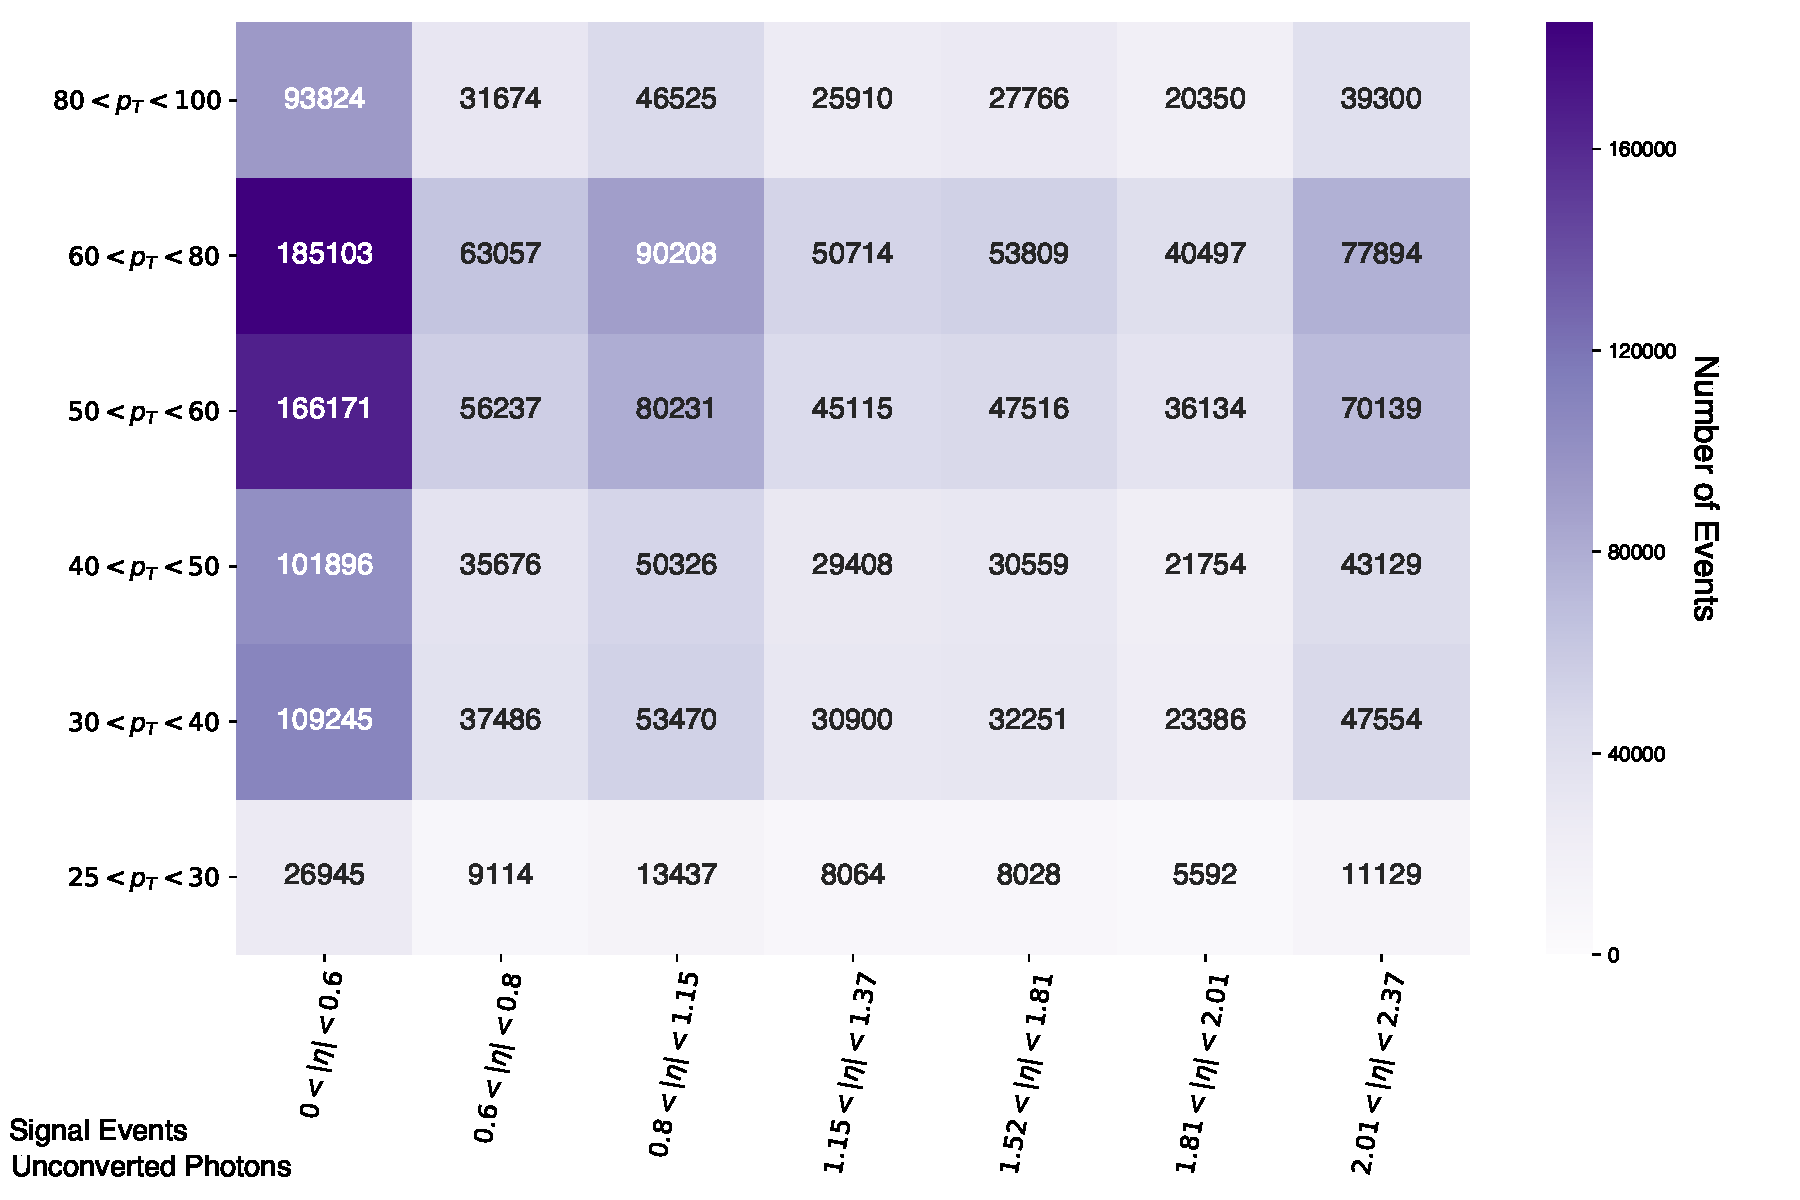
\includegraphics[width=.85\textwidth]{chapters/chapter4_photonID/images/sig_events.pdf}
    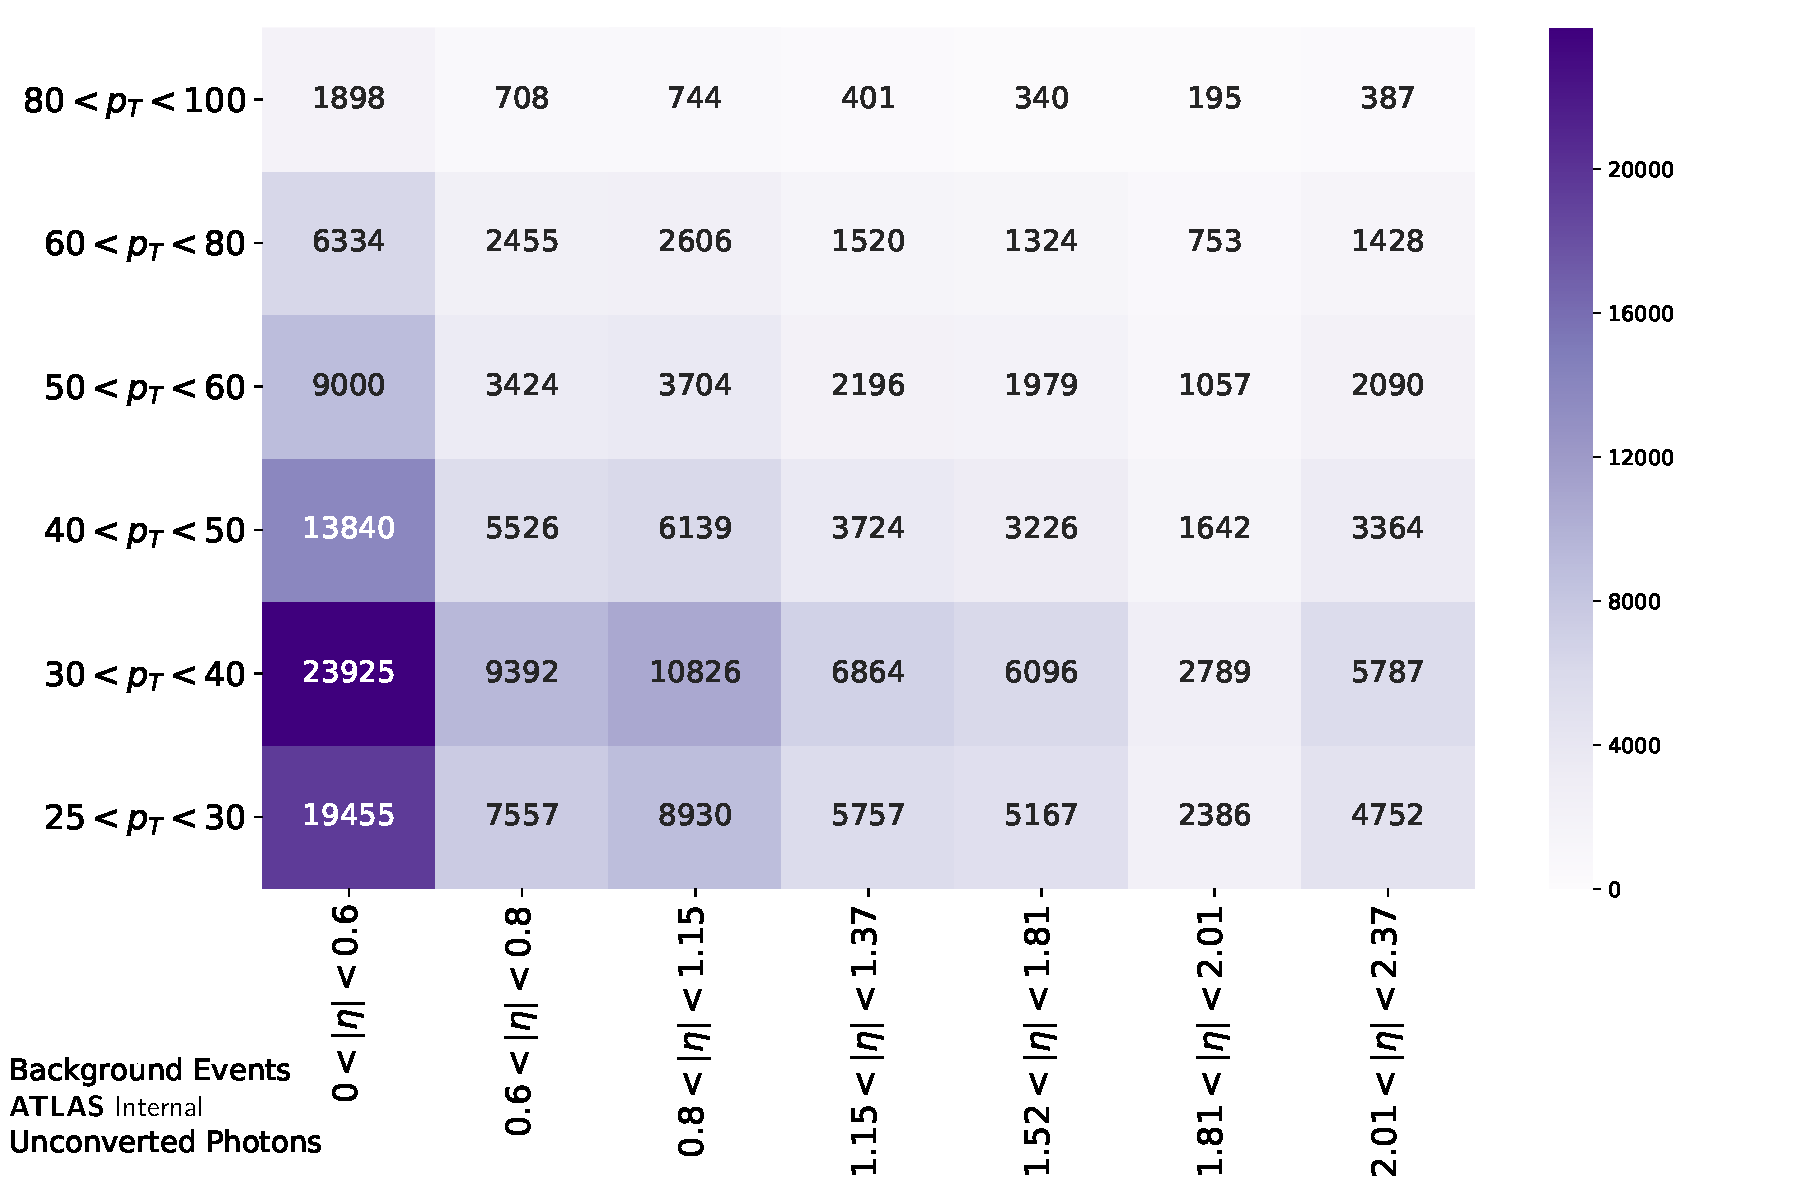
\includegraphics[width=.85\textwidth]{chapters/chapter4_photonID/images/bkg_events.pdf}
    \caption[Number of training events used in the model for unconverted photons in each $\eta$-\pt bin for the signal $\gamma$+jets sample, and the background jet fakes sample]{Number of training events used in the model for unconverted photons in each $\eta$-\pt bin for the signal $\gamma$+jets sample (top), and the background jet fakes sample (bottom). The preselection described in Section \ref{sec:photon-id-samples} is used.}
    \label{fig:photonid-events}
\end{figure}

\begin{figure}[!thp]
    \centering
    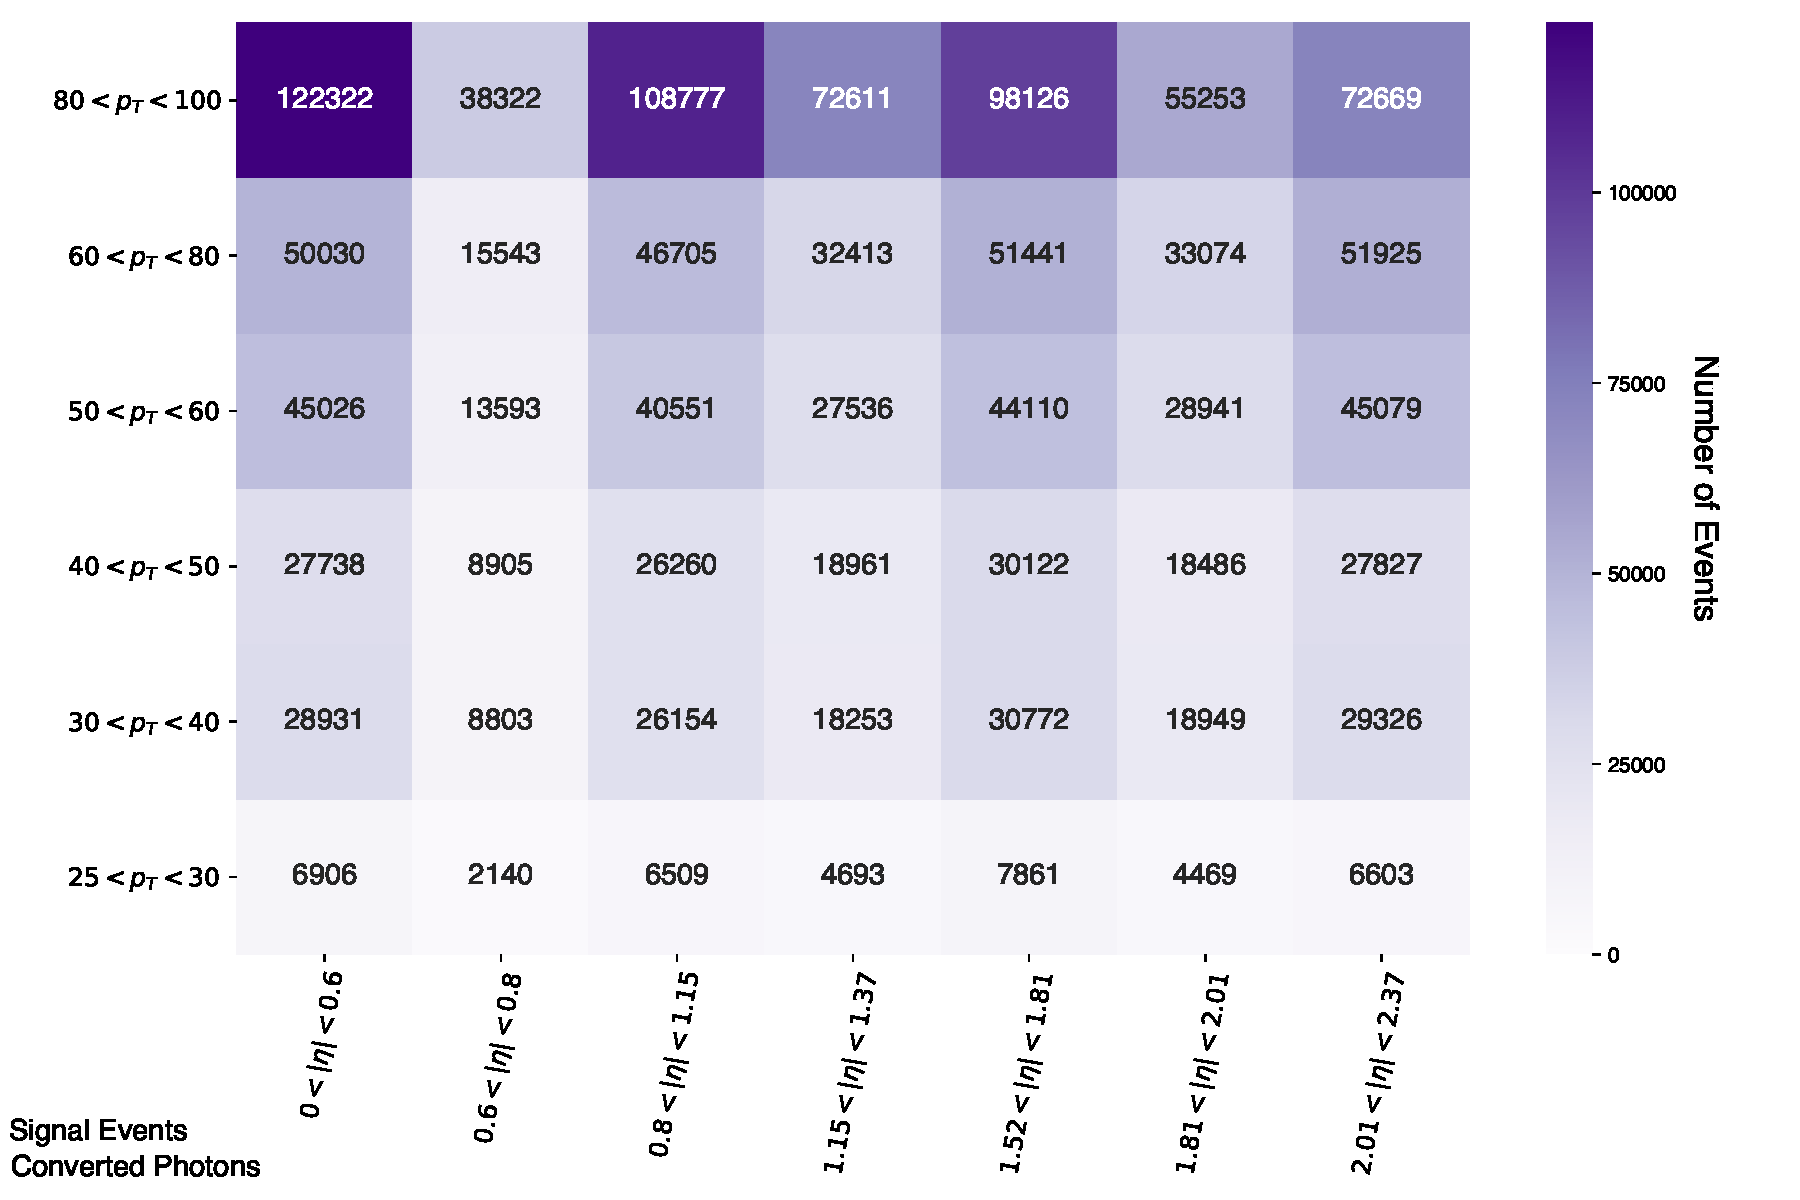
\includegraphics[width=.85\textwidth]{chapters/chapter4_photonID/images/conv_sig_events.pdf}
    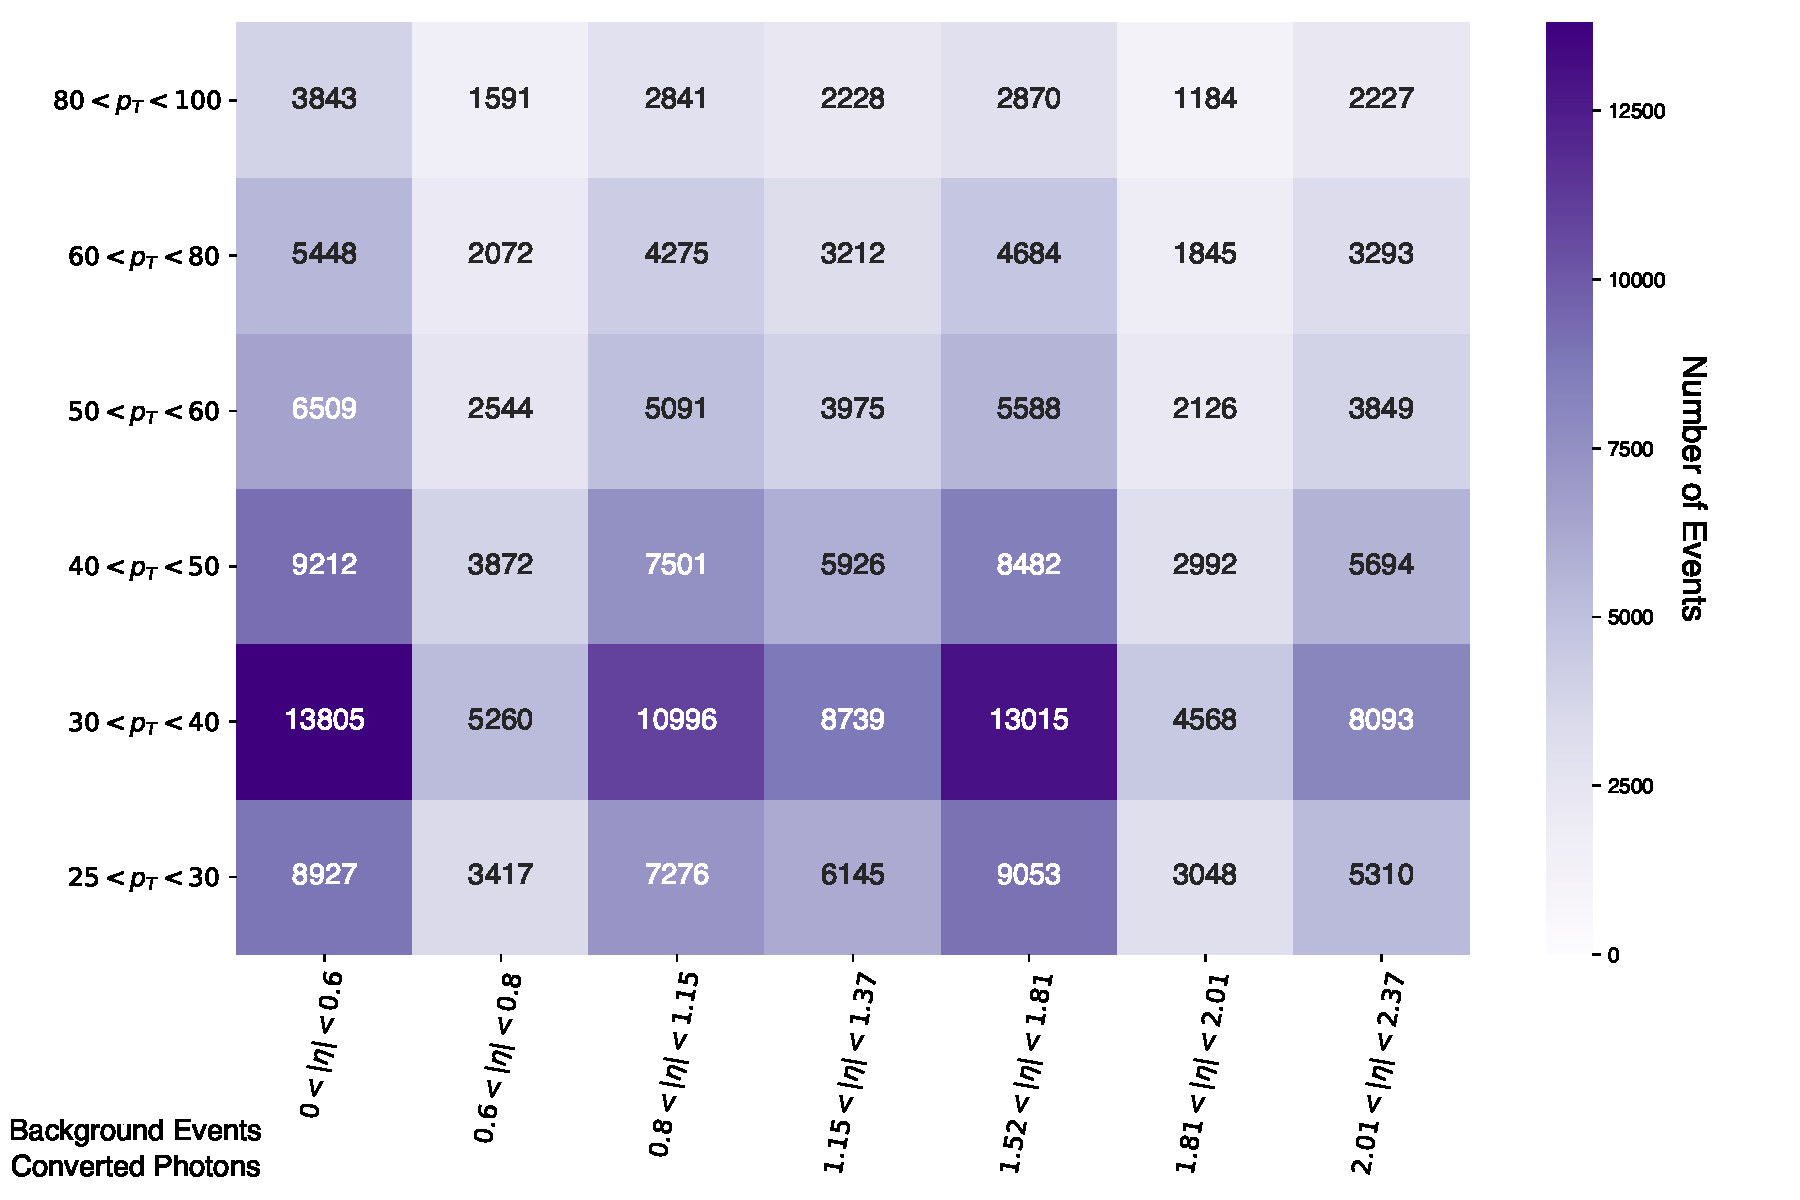
\includegraphics[width=.85\textwidth]{chapters/chapter4_photonID/images/conv_bkg_events.pdf}
    \caption[Number of training events used in the model for converted photons in each $\eta$-\pt bin for the signal $\gamma$+jets sample, and the background jet fakes sample]{Number of training events used in the model for converted photons in each $\eta$-\pt bin for the signal $\gamma$+jets sample (top), and the background jet fakes sample (bottom). The preselection described in Section \ref{sec:photon-id-samples} is used.}
    \label{fig:conv-photonid-events}
\end{figure}

\begin{figure}[!th]
    \centering
    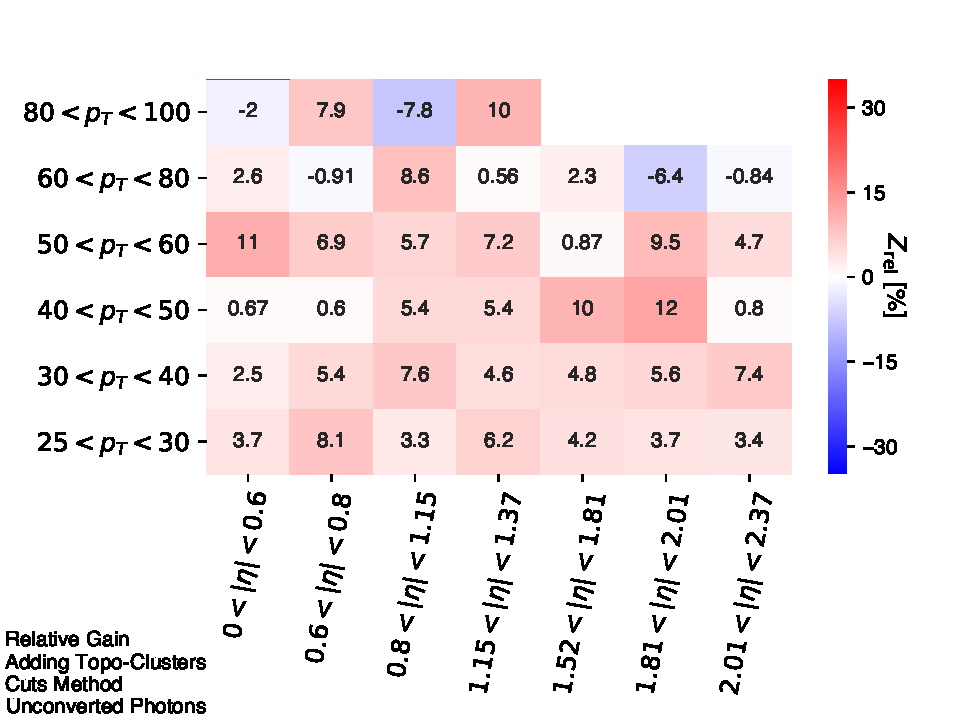
\includegraphics[width=.85\textwidth]{chapters/chapter4_photonID/images/gain_topoAdded_unconverted.pdf}
    \caption[The relative gain in background rejection, $Z_{\text{rel}}$, for each $\eta-\pt$ bin at 85\% signal efficiency by adding topo-cluster moment variables into the cut-based photon identification menu]{The relative gain in background rejection, $Z_{\text{rel}}$, for each $\eta-\pt$ bin at 85\% signal efficiency by adding topo-cluster moment variables into the cut-based photon identification menu. Bins with fewer than 400 background events are masked.}
    \label{fig:gain-topo-clusters-added-unconverted}
\end{figure}


\section{Multivariate Analysis Techniques}

The current photon identification working points are defined by a rectangular cuts method. Cut optimization is performed through a 9-dimensional scan over the shower shape variables. In order to better reject background, a multivariate approach to defining these working points has been investigated. These methods are outlined in detail in Appendix \ref{app:MVA}, and the following sections will discuss the improvements brought to photon identification through implementing them.

\subsection{Boosted Decision Tree}

A gradient boosted \gls{BDT} was employed as an alternative classification algorithm. A major problem in training these \glspl{BDT} was the lack of background training statistics when segmenting into $\eta$-\pt bins. To navigate this problem, rather than training an independent model for each $\eta$-\pt bin, \pt inclusive models were trained. As shown in Figure \ref{fig:photonid-corrs}, the input variables have low correlation to \pt, and thus this does not bias the model. This provided better performance in high \pt bins. In low \pt bins, it provided better performance overall, but in a few bins had equivalent or negligibly worse performance. The percent improvement, as defined using the same metric defined in \ref{eqn:improvement-metric}, is shown in Figure\ref{fig:bdtinclusive-vs-bdt}, with the bin-wise trained \gls{BDT} used as the baseline.

\begin{figure}[!th]
    \centering
    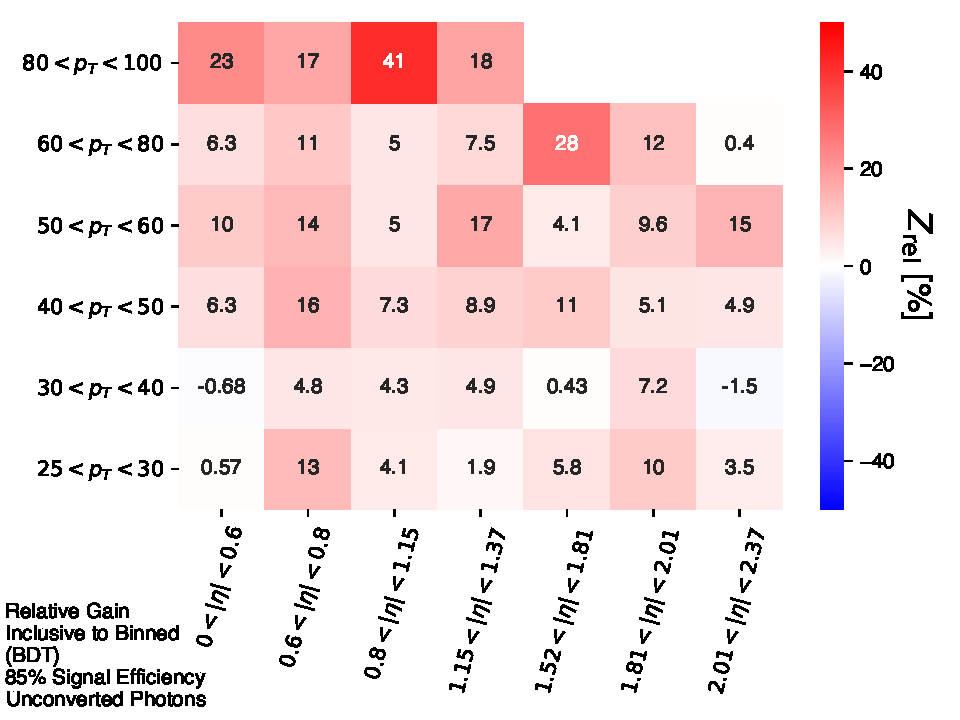
\includegraphics[width=.85\textwidth]{chapters/chapter4_photonID/images/BDTInclusive_v_BDT_normed.pdf}
    \caption[The relative improvement in background rejection by using a \pt-inclusive trained \gls{BDT} compared to a \pt-binned \gls{BDT}]
    {The relative improvement in background rejection, $Z_{\text{rel}}$, for each $\eta-\pt$ bin at 85\% signal efficiency by using a \pt-inclusive trained \gls{BDT} compared to a \pt-binned \gls{BDT}. Only shower-shape variables are included as inputs. Bins with fewer than 400 background events are masked.}
    \label{fig:bdtinclusive-vs-bdt}
\end{figure}


As a baseline, the \gls{BDT} is compared to the cut-based photon identification menu, using the same figure of merit defined in Equation \ref{eqn:improvement-metric}, where the efficiency denoted $i$ represents the \gls{BDT} model, and the efficiency denoted $0$ represents the current cut-based model. This model performs better, except in the two most outer $\eta$ bins, shown in Figure \ref{fig:gain-bdt-vs-cuts}.


\begin{figure}[!th]
    \centering
    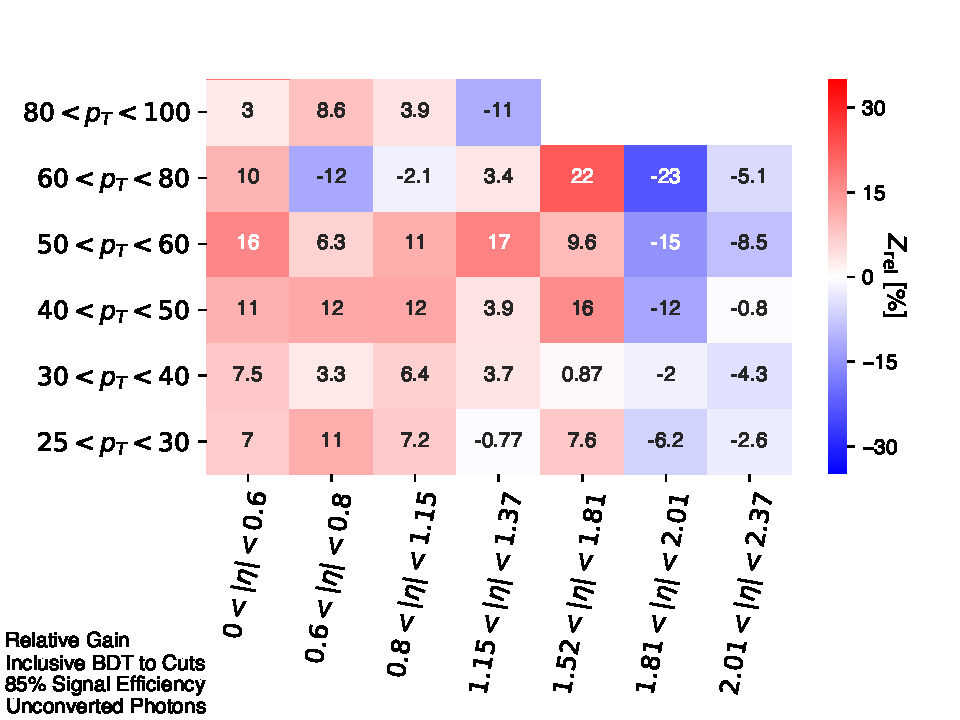
\includegraphics[width=.85\textwidth]{chapters/chapter4_photonID/images/gain_BDTinclusive_cuts_unconverted.pdf}
    \caption[The relative gain in background rejection, $Z_{\text{rel}}$, for each $\eta-\pt$ bin at 85\% signal efficiency by using a \gls{BDT} compared to the cut-based photon identification menu]
    {The relative gain in background rejection, $Z_{\text{rel}}$, for each $\eta-\pt$ bin at 85\% signal efficiency by using a \gls{BDT} compared to the cut-based photon identification menu. Only shower-shape variables are included as inputs. Bins with fewer than 400 background events are masked.}
    \label{fig:gain-bdt-vs-cuts}
\end{figure}


\subsection{Neural Network}

In addition to a \gls{BDT}, a \gls{NN} was studied for photon classification, considering the same shower shape variables. It was developed using Keras \cite{Keras} using the Tensorflow \cite{Tensorflow} backend. The model topology\footnote{A description of \gls{NN} topologies, activation functions, and other associated terminology can be found in Appendix \ref{app:MVA}.} used is shown in Figure \ref{fig:nn-model}, it has an input layer of size 9 to match the number of shower shape variables, which is densely connected to a hidden layer of size 6, with ReLU activation functions. This layer is densely connected to an output, where a dropout \cite{dropout} of 20\% is used while training to reduce overtraining. This produces a total of 67 trainable parameters.

\begin{figure}
    \centering
    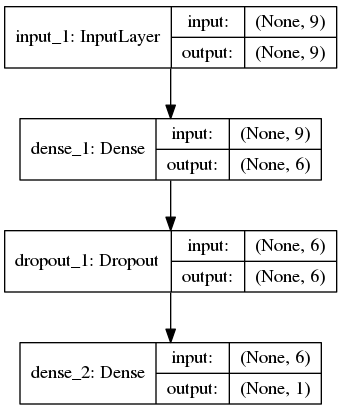
\includegraphics[width=.30\textwidth]{chapters/chapter4_photonID/images/model.png}
    \caption[A diagram of the \gls{NN} topology used for photon identification]
    {A diagram of the \gls{NN} topology used for photon identification. Inputs to this \gls{NN} are the shower shape variables.}
    \label{fig:nn-model}
\end{figure}


For unconverted photons, the \gls{NN} performed better at low \pt than the inclusively trained \gls{BDT}, but worse at high \pt. This comparison can be seen in Figure \ref{fig:nn-v-bdt-unconverted}. A \pt-inclusive training approach was considered for the \gls{NN} as well, however provided a worse performance for the majority of $\eta-\pt$ bins, shown in Figure \ref{fig:nninclusive-v-binned}.

\begin{figure}
    \centering
    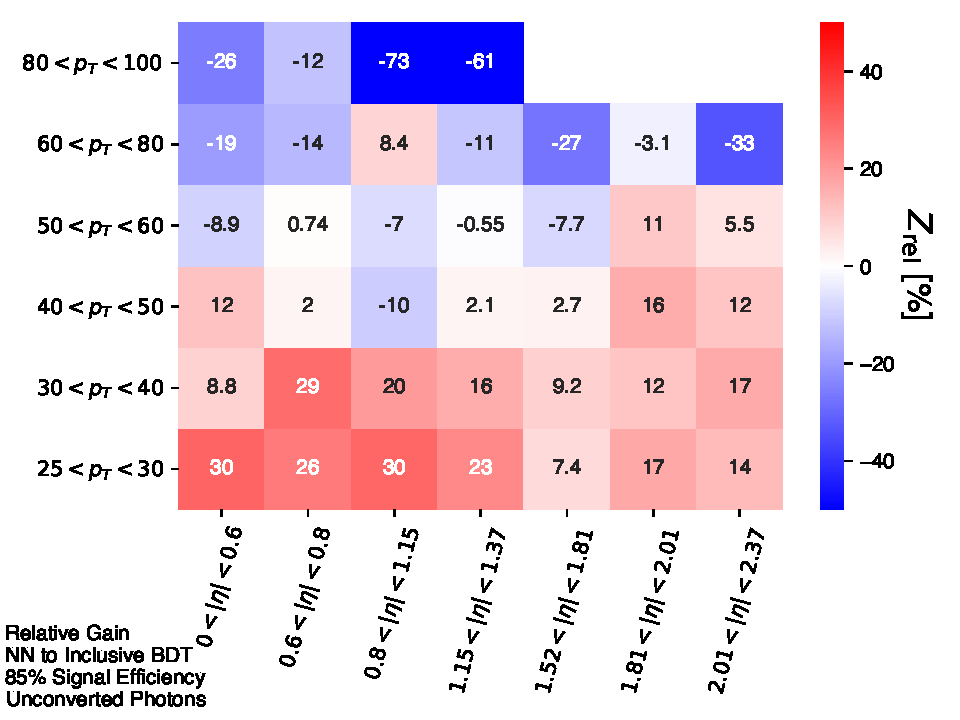
\includegraphics[width=.85\textwidth]{chapters/chapter4_photonID/images/NN_v_BDTinclusive_normed.pdf}
    \caption[The relative gain in background rejection by using a \gls{NN} trained bin-wise compared to a \gls{BDT} trained inclusively]
    {The relative gain in background rejection, $Z_{\text{rel}}$, for each $\eta-\pt$ bin at 85\% signal efficiency by using a \gls{NN} trained in each $\eta-\pt$ bin compared to a \gls{BDT} trained inclusively. Negative values can be interpreted as the \gls{BDT} having better performance than the \gls{NN}. Only shower-shape variables are included as inputs for both models. Bins with fewer than 400 background events are masked.}
    \label{fig:nn-v-bdt-unconverted}
\end{figure}


\begin{figure}
    \centering
    \includegraphics[width=.85\textwidth]{chapters/chapter4_photonID/images/NNinclusive_v_NN_normed.pdf}
    \caption[The relative gain in background rejection by using a \gls{NN} trained inclusively compared to one trained bin-wise]
    {The relative gain in background rejection, $Z_{\text{rel}}$, for each $\eta-\pt$ bin at 85\% signal efficiency by using a \gls{NN} trained inclusively compared to one trained in each $\eta-\pt$ bin. Negative values can be interpreted as the bin-wise training having better performance than the inclusive training. Only shower-shape variables are included as inputs for both models. Bins with fewer than 400 background events are masked.}
    \label{fig:nninclusive-v-binned}
\end{figure}



\subsection{MVA With Topo-Cluster Variables}

The \gls{BDT} was also studied incorporating the topo-cluster moments as inputs. This 
\chapter{Search for di-Higgs Production in the $\gamma\gamma b\bar{b}$ Channel} % todo: yybb not capitalized?

\section{Analysis Overview}

This analysis searches for resonant and non-resonant di-Higgs production, where one Higgs boson decays to a pair of photons, and the other decays to a \bb pair. The motivation for searching for di-Higgs production is outlined in Section \ref{sec:diHiggs}. Di-Higgs production provides a direct probe of the Higgs trilinear coupling. This decay channel, \yybb, is appealing to study due to the clean diphoton trigger, relatively small backgrounds, and excellent diphoton mass resolution. Enhancements to the di-Higgs rate may be observable in the current \RunTwo dataset, and realized through a resonance or non-resonantly. The resonant search looks for a generic scalar, and thus is model independent, however this scalar may be realized as a heavy Higgs in a \gls{THDM} \cite{THDM}. Non-resonantly, enhancements can occur through the presence of \gls{BSM} couplings.


Previous results were presented with an integrated luminosity of 20 \ifb at $\sqrt{s}=\unit{8}{\TeV}$ representing ATLAS dataset in 2012. In this, a 2.4$\sigma$ excess was observed \cite{yybb-2015}. This was followed by a search encompassing early \RunTwo data, just that taken in 2015, corresponding to 3.2 \ifb at $\sqrt{s}=\unit{13}{\TeV}$ \cite{run2_2015}. This search used the same object selection as the \RunOne analysis, and a common selection between the resonant and non-resonant analysis. No significant excesses were seen.

The presented analysis expands on the prior analyses, using \RunTwo data from 2015-2016 corresponding to 36.1 \ifb. A new event selection is defined to be sensitive to the \RunTwo conditions. Furthermore, the previous cut-and-count approach has been replaced by a fit procedure. In the resonant analysis, this is performed on the \myybb distribution after cutting on \myy to isolate $H\rightarrow \gamma \gamma$ events. In the non-resonant analysis the fit is performed on the \myy spectrum. Chapter \ref{ch:vbf} will then present future updates to this analysis.


\section{Data and Simulated Samples}


\subsection{Data}

The analysis presented uses $pp$ collision data recorded by the ATLAS experiment at the LHC in 2015 and 2016, the first half of ``Run 2.'' After detector and data quality requirements, the total collected data corresponds to 36.1 \ifb. A loose diphoton trigger is used for this search, \texttt{HLT\_g35\_loose\_g25\_loose}, which triggers on diphoton events where the leading (subleading) photon \pt is greater than 35\% (25\%) the diphoton invariant mass.

\subsection{Simulated Samples}

Simulation is generated as outlined in Chapter \ref{ch:eventreco} in order to compare theoretical predictions to data. Independent samples are made for the considered signal hypotheses (outlined in Section \ref{sssec:signal-samples}), as well as for the predominant backgrounds (outlined in Section \ref{sssec:background-samples}).

\subsubsection{Signal Samples} \label{sssec:signal-samples}

This analysis considers two signal sources: non-resonant di-Higgs production and resonant production of Higgs boson pairs through a scalar resonance. In addition to \gls{SM} non-resonant signal samples, samples with varied \klambda are produced. This section describes the \gls{MC} samples used to model these various signal processes.\\

\noindent\textbf{Non-resonant \gls{SM} Signal Samples}\\
\indent The non-resonant di-Higgs signal sample corresponding to \gls{SM} \gls{ggF} \hh production is generated at \gls{NLO} in \gls{QCD}. The model was developed within the Cosmology, Particle Physics, and Phenomenology (CP3) theory group \cite{top-quark-massrw}, and is known as FT\textsubscript{approx}. It generates events in a Higgs \gls{EFT} by using the \AMCatNLO method \cite{amc-at-nlo}.

An event reweighting is applied to account for top-quark mass dependence. Due to interference between the box and triangle diagrams, this is an important effect (documented, for example, in Reference \cite{top-quark-mass-example}). All exact one-loop amplitudes and known exact two-loop amplitudes are used. For the \gls{NNLO} normalization, these effects are of order 5\%.

The sample used is showered using \HERWIGpp \cite{herwigpp}, using the \texttt{UEEE5} tune and the \texttt{CTEQ6L1} PDF set.
%% include LO comparison plots from note?


\noindent\textbf{Non-resonant Varied \klambda Signal Samples}\\
\indent Samples for non-resonant di-Higgs production with varied \klambda were generated at values $\klambda = 0, \pm 1, \pm 2, \pm 4, \pm 6, \pm 10$. These samples were generated at \gls{LO}, then reweighted to \gls{NNLO} through a $K$-factor, taking the ratio of the cross-sections of the FT\textsubscript{approx} \gls{SM} non-resonant signal sample (at \gls{NNLO}) and the $\klambda =1$ sample (at \gls{LO}).

For generic \klambda, an interpolation function can be used to predict the amplitude, and thus the signal yield. The amplitude can be written as

\begin{equation}
  A(k_t,\klambda) = k_t^2 B + k_t \klambda T,
\end{equation}
%
where $B$ is the contribution from the box diagram (with two $th$ vertices, thus squared) and $T$ is the contribution from the trilinear diagram (containing one $th$ and one $hhh$ vertex). Squaring this amplitude and varying \klambda (consider values 0, 1, and 10) gives

\begin{align}
  &|A(k_t,\klambda)|^2 = k_t^4 |B|^2 + k_t^2\klambda^2 |T|^2 + k_t^3\klambda(B^*T + BT^*)\\
  &|A(1,0)|^2 = |B|^2\\
  &|A(1,1)|^2 = |B|^2 + |T|^2 + (B^*T + BT^*)\\
  &|A(1,10)|^2 = |B|^2 + 100|T|^2 + 10(B^*T + BT^*).
\end{align}
%
These equations can then be combined to express the squared amplitude in terms of the amplitudes of the varied reference samples for any arbitrary $\klambda$ and $k_t$,
\begin{equation}
  |A(k_t,\klambda)|^2 = k_t^2 \left[ 
    \frac{90 k_t^2 + 9\klambda^2 - 99k_t\klambda}{90}|A(1,0)|^2 +
    \frac{100 k_t\klambda - 10\klambda^2}{90}|A(1,1)|^2 +
    \frac{\klambda^2 - k_t\klambda}{90}|A(1,1)|^2 \right].
\end{equation}
% todo : add to appendix validation plots?

\noindent\textbf{Resonant Signal Samples}\\
\indent The resonant samples were generated using a model of a heavy scalar decaying to two Higgs bosons, with the narrow-width approximation ($\unit{10}{\MeV}$ is used). A $gg$-initiated state is generated at NLO using \AMCatNLO, and the scalar is forced to decay to two \gls{SM} Higgs bosons with $m_H = \unit{125}{\GeV}$. Showering is performed in \HERWIGpp using the \texttt{CT10 NLO} \gls{PDF} set and \texttt{UEEE5} tuned parameters. To ensure the final state is \yybb, the \path{XtoVVDecayFilter} is used. Samples are generated at the following scalar mass hypotheses (in GeV): 260, 275, 325, 350, 400, 450, 500, 750, 1000.


\subsubsection{Background Samples}\label{sssec:background-samples}

The dominant background in this analysis are the non-resonant \myy continuum events. Additionally, mono-Higgs boson production is a subdominant background to this analysis, which is composed of several production modes ($ggH$, VBF $H$, $ZH$, $WH$, $tH$, $ttH$, $bbH$). This section describes the samples used to model these background processes.\\

\noindent\textbf{\yy-Continuum}\\
\indent \yy-continuum processes including two photons and jets are generated using \SHERPA. This \gls{MC} sample is used predominantly for shape information, since normalization is taken through a data-driven approach using the diphoton sidebands. Jets faking photons are also modeled from the data sidebands using a template fit, described in Section \ref{ssec:background-composition}.\\

\noindent\textbf{Mono-Higgs Production}\\
\indent The following mono-Higgs production channels are considered: gluon-gluon fusion ($ggH$), vector-boson fusion (VBF $H$) $Z$-associated production ($ZH$), $W$-associated production ($WH$), single and top quark pair associated production ($tH$ and \tth, respectively), and bottom quark pair associated production ($bbH$)\footnote{There are two $bbH$ samples in order to account for interference.}. Rates for these samples are taken from the 2016 Yellow Report \cite{yellow-report}. The generators for these samples vary, and are listed in Table \ref{tab:single-higgs-samples}, along with the cross-section times \gls{BR} for each sample.

\begin{table}[htbp]
  \begin{center}
    \caption[Mono-Higgs boson backgrounds considered, including generator and PDF used to produce each sample]{Mono-Higgs boson backgrounds considered, including generator and PDF used to produce each sample. Cross-section for each sample is shown, multiplied by the $H\rightarrow \gamma\gamma$ \gls{BR} of 0.00227. Cross-sections assume $\sqrt{s}=\unit{13}{\TeV}$ and $m_{H}=\unit{125}{\GeV}$.}
    \label{tab:single-higgs-samples}
    \begin{tabular}{|c|c|c|}
      \hline
      Process & Generator+PDF & $\sigma \times \mathcal{B}\ (H\rightarrow\gamma\gamma)$ \\
      \hline
      $ggH$ & \makecell{\POWHEG+ \peight \\ PDF4LHC15}& 0.1101404\\
      \hline
      VBF $H$ & \makecell{\POWHEG+ \peight \\ PDF4LHC15}& 0.00857833\\
      \hline
      $W^-H$ & \makecell{\POWHEG+ \peight \\ PDF4LHC15}& 0.00120605\\
      \hline
      $W^+H$ & \makecell{\POWHEG+ \peight \\ PDF4LHC15}& 0.00190226\\
      \hline
      $ZH$ & \makecell{\POWHEG+ \peight \\ PDF4LHC15}& 0.001724519\\
      \hline
      $ggZH$ & \makecell{\POWHEG+ \peight \\ PDF4LHC15}& 0.000278529\\
      \hline
      \tth & \makecell{\peight \\ A14 NNPDF23LO}& 0.001149755\\
      \hline
      $bbH$ (positive) & \makecell{\AMCatNLO+ \peight \\ A14 NNPDF23LO}& 0.00110390\\
      \hline
      $bbH$ (negative) & \makecell{\AMCatNLO+ \peight \\ A14 NNPDF23LO}& -8.95378e-05\\
      \hline
      $tH$ ($t$-channel) & \makecell{\MADGRAPH+ \peight \\ A14 CT10ME}& 0.00016857\\
      \hline
      $tH$ ($W$-associated) & \makecell{\AMCatNLO+ \peight \\ UEEE5 CTEQ6L1 CT10ME}& 3.44359e-05\\
      \hline
    \end{tabular}
  \end{center}
\end{table}


\section{Object Definition}
\subsection{Photons}

Selected photons for this analysis are converted or unconverted photons which pass tight ID cuts (outlined in Section \ref{ssec:em-signatures}). Photons must have $\pt > \unit{25}{\GeV}$ and $\abseta < 2.37$. Additionally, the crack region of $1.37 < \abseta < 1.52$ is rejected.

Isolation criteria are set on $E_{\text{T}}^{\text{iso}}$ and $p{\text{T}}^{\text{iso}}$. $E_{\text{T}}^{\text{iso}}$ is the calorimeter-based isolation, the sum of energy of all topological clusters in $\Dr = 0.2$ of a photon candidate. $p{\text{T}}^{\text{iso}}$ is the track-based isolation, the sum of the transverse momenta of all tracks with $\pt > \unit{1}{\GeV}$ within $\Dr = 0.2$ of the candidate. Photon candidates must have $E_{\text{T}}^{\text{iso}}$ less than 6.5\% of their transverse energy, and $p{\text{T}}^{\text{iso}}$ less than 5\% of their transverse energy\footnote{Known as the FixedCutLoose working point.}. This requirement is 98\% efficient. 


Photons must pass an ambiguity tool that reduces the large $e\rightarrow\gamma$ fake rates from converted photons. This differentiates overlapping selections by making additional requirements on silicon hits and conversion rates \cite{r1-photonID}.

The leading photon \pt distribution is shown in Figure \ref{fig:photon_l_pt}, the subleading is shown in Figure \ref{fig:photon_s_pt}.

\begin{figure}[p]
  \centering
  \includegraphics[width=0.48\textwidth]{chapters/chapter5_yybb/images/data_MC_comparison/h_CR_l_0t_nominal_leadingPhoton_pt.pdf}
  \includegraphics[width=0.48\textwidth]{chapters/chapter5_yybb/images/data_MC_comparison/h_CR_h_0t_nominal_leadingPhoton_pt.pdf}
  \includegraphics[width=0.48\textwidth]{chapters/chapter5_yybb/images/data_MC_comparison/h_SR_l_1t_nominal_leadingPhoton_pt.pdf}
  \includegraphics[width=0.48\textwidth]{chapters/chapter5_yybb/images/data_MC_comparison/h_SR_h_1t_nominal_leadingPhoton_pt.pdf}
  \includegraphics[width=0.48\textwidth]{chapters/chapter5_yybb/images/data_MC_comparison/h_SR_l_2t_nominal_leadingPhoton_pt.pdf}
  \includegraphics[width=0.48\textwidth]{chapters/chapter5_yybb/images/data_MC_comparison/h_SR_h_2t_nominal_leadingPhoton_pt.pdf}
  \caption[Leading photon \pt.]{Leading photon \pt by b-tagging category. The low (left) and high (right) mass selections are shown. Both data and MC are normalized such that the integral is 1.
  \label{fig:photon_l_pt}}
\end{figure}

\begin{figure}[p]
  \centering
  \includegraphics[width=0.48\textwidth]{chapters/chapter5_yybb/images/data_MC_comparison/h_CR_l_0t_nominal_subleadingPhoton_pt.pdf}
  \includegraphics[width=0.48\textwidth]{chapters/chapter5_yybb/images/data_MC_comparison/h_CR_h_0t_nominal_subleadingPhoton_pt.pdf}
  \includegraphics[width=0.48\textwidth]{chapters/chapter5_yybb/images/data_MC_comparison/h_SR_l_1t_nominal_subleadingPhoton_pt.pdf}
  \includegraphics[width=0.48\textwidth]{chapters/chapter5_yybb/images/data_MC_comparison/h_SR_h_1t_nominal_subleadingPhoton_pt.pdf}
  \includegraphics[width=0.48\textwidth]{chapters/chapter5_yybb/images/data_MC_comparison/h_SR_l_2t_nominal_subleadingPhoton_pt.pdf}
  \includegraphics[width=0.48\textwidth]{chapters/chapter5_yybb/images/data_MC_comparison/h_SR_h_2t_nominal_subleadingPhoton_pt.pdf}
  \caption[Subleading photon \pt.]{Subleading photon \pt by b-tagging category. The low (left) and high (right) mass selections are shown. Both data and MC are normalized such that the integral is 1.
  \label{fig:photon_s_pt}}
\end{figure}

To select the \gls{PV}, a \gls{NN} is used. This \gls{NN} uses the following inputs:
\begin{itemize}
  \item $(z_{\text{common}} - z_{\text{vertex}})/(\sigma_z)$. $z_{\text{vertex}}$ is the position of the primary vertex. $z_{\text{common}}$ is defined by the weighted mean of extrapolated photon trajectories. For converted photons, this is replaced by the direction derived by connecting the conversion location to the cluster barycenter in the first sampling layer in the \gls{EM} calorimeter. $\sigma_z$ is the associated error.
  \item $\log(\sum \pt)$ of tracks
  \item $\log(\sum \pt^2)$ of tracks
  \item $\Delta \phi(\gamma\gamma,\text{PV})$. $\phi$ of the \gls{PV} is defined as the $\phi$ vector sum of tracks associated to the vertex
  
\end{itemize}
After selecting this \gls{PV}, tracking and calorimeter variables are recomputed with respect to the new chosen \gls{PV}. This method is greater than 85\% efficient at selecting the correct \gls{PV}.


\subsection{Electrons}

Electrons are used to reject jets originating from leptons. Electrons are required to have $\pt > \unit{10}{\GeV}$, and $\abseta < 2.47$ and outside of the crack-region ($1.37 < \abseta < 1.52$). They must pass medium identification and loose isolation requirements, which are set on both calorimeter and tracking variables and are 99\% efficient.

\subsection{Jets}

Jets are reconstructed with the \path{FastJet} \cite{fastjet} package. They are defined using the \antikt algorithm with $R=0.4$, using jets with energy corrected for pile-up effects and direction readjusted to the primary vertex (EM-JES jets). Jets considered must have $\pt > \unit{25}{\GeV}$ and be within the tagging region, $\abseta < 2.5$. The following additional requirements are applied\footnote{This selection is similar to that of the default jet selection for ATLAS $H\rightarrow \yy$ analyses. The $\abseta < 2.5$ is an additional requirement imposed atop that selection for b-tagging.}:

\begin{itemize}
  \item Jets with $\pt < \unit{50}{\GeV}$ and $\abseta < 2.4$ must pass the ``default'' \gls{JVT} requirement, with $|\text{JVT}| \geq 0.59$ \cite{JVT}.
  \item Events that contain a jet passing the ``LooseBad'' cut are vetoed. 
  \item Jets with $\Dr < 0.4$ from a tight, isolated photon are vetoed.
  \item Jets with $\Dr < 0.2$ from a selected electron are vetoed.
\end{itemize}



Following this selection, candidate jets are selected in the following way:
\begin{itemize}
  \item In the 0-tag control region, the two leading jets are the candidate jets.
  \item In the 1-tag region, one of the jets is the b-tagged jet, the other is selected via a \gls{BDT}
  \item In the 2-tag region, the two b-tagged jets are the candidate jets.
\end{itemize}

\begin{figure}[p] %TODO cite me
  \centering
  \includegraphics[width=0.48\textwidth]{chapters/chapter5_yybb/images/data_MC_comparison/h_CR_l_0t_nominal_leadingJet_pt.pdf}
  \includegraphics[width=0.48\textwidth]{chapters/chapter5_yybb/images/data_MC_comparison/h_CR_h_0t_nominal_leadingJet_pt.pdf}
  \includegraphics[width=0.48\textwidth]{chapters/chapter5_yybb/images/data_MC_comparison/h_SR_l_1t_nominal_leadingJet_pt.pdf}
  \includegraphics[width=0.48\textwidth]{chapters/chapter5_yybb/images/data_MC_comparison/h_SR_h_1t_nominal_leadingJet_pt.pdf}
  \includegraphics[width=0.48\textwidth]{chapters/chapter5_yybb/images/data_MC_comparison/h_SR_l_2t_nominal_leadingJet_pt.pdf}
  \includegraphics[width=0.48\textwidth]{chapters/chapter5_yybb/images/data_MC_comparison/h_SR_h_2t_nominal_leadingJet_pt.pdf}
  \caption[Leading jet \pt.]{Leading jet \pt by b-tagging category. The low (left) and high (right) mass selections are shown. Both data and MC are normalized such that the integral is 1.
  \label{fig:jet_l_pt}}
\end{figure}

\begin{figure}[p]
  \centering
  \includegraphics[width=0.48\textwidth]{chapters/chapter5_yybb/images/data_MC_comparison/h_CR_l_0t_nominal_subleadingJet_pt.pdf}
  \includegraphics[width=0.48\textwidth]{chapters/chapter5_yybb/images/data_MC_comparison/h_CR_h_0t_nominal_subleadingJet_pt.pdf}
  \includegraphics[width=0.48\textwidth]{chapters/chapter5_yybb/images/data_MC_comparison/h_SR_l_1t_nominal_subleadingJet_pt.pdf}
  \includegraphics[width=0.48\textwidth]{chapters/chapter5_yybb/images/data_MC_comparison/h_SR_h_1t_nominal_subleadingJet_pt.pdf}
  \includegraphics[width=0.48\textwidth]{chapters/chapter5_yybb/images/data_MC_comparison/h_SR_l_2t_nominal_subleadingJet_pt.pdf}
  \includegraphics[width=0.48\textwidth]{chapters/chapter5_yybb/images/data_MC_comparison/h_SR_h_2t_nominal_subleadingJet_pt.pdf}
  \caption[Subleading jet \pt.]{Leading jet \pt by b-tagging category. The low (left) and high (right) mass selections are shown. Both data and MC are normalized such that the integral is 1.
  \label{fig:jet_s_pt}}
\end{figure}


In order to reconstruct the 4-body mass, $m_{\gamma\gamma jj}$, in cases where there are not 2 $b$-tagged jets, an additional candidate jet is selected through the use of a \gls{BDT}. The inputs to this \gls{BDT} are: jet and dijet \pt, dijet mass, jet and dijet $\eta$, dijet \Deta, booleans for passing the 77\% and 85\% \btagging WP, and the ranking of the jets in terms of:

\begin{itemize}
  \item Highest jet \pt
  \item Lowest $\Delta m = m_{bb} - m_H$ when summed with the $b$-tagged jet
  \item Highest dijet \pt, when summed with the $b$-tagged jet
\end{itemize}

The jet with the highest \gls{BDT} score is selected as the pairing when constructing  $m_{\gamma\gamma jj}$. The performance is better at high mass hypotheses, since the signal shape is more pronounced from the background than at low masses. 

% TODO: ADD plots


\subsection{Muons}

In jet reconstruction, a muon-in-jet correction is used to improve resolution for $b$-jets. This accounts for leptonic decays involving muons which do not entirely deposit their energy in the \gls{EM} or hadronic calorimeters. Muons must pass medium requirements, have $\pt > \unit{4}{\GeV}$, $\abseta < 2.7$, $|d_{0}|$ significance less than 3, $|z_{0}|$ less than 0.5 mm\footnote{Both $|d_{0}|$ and $|z_{0}|$ requirements are with respect to the primary vertex.}.

For correcting the $b$-jets, the 4-momenta of all muons within the jet's \Dr cone are added to the $b$-jet. Adding this correction shifts the $m_{bb}$ distribution closer to the Higgs mass and provides a $5-6\%$ improvement in signal acceptance for each resonant mass point. Figure \ref{fig:n_muons} shows the number of muons added to each jet, typically 0 or 1 muon.

\begin{figure}[!ht]
  \centering
  \includegraphics[height=0.32\textwidth]{chapters/chapter5_yybb/images/muon-in-jet/all_mu_n_allMu_low_1.pdf}
  \includegraphics[height=0.32\textwidth]{chapters/chapter5_yybb/images/muon-in-jet/all_mu_n_allMu_low_2.pdf} \\
  \includegraphics[height=0.32\textwidth]{chapters/chapter5_yybb/images/muon-in-jet/all_mu_n_allMu_high_1.pdf}
  \includegraphics[height=0.32\textwidth]{chapters/chapter5_yybb/images/muon-in-jet/all_mu_n_allMu_high_2.pdf} \\
  \caption[Number of muons added to each jet, shown for each $b$-tagging category with the low and high mass  selections applied]{Number of muons added to each jet, shown for each $b$-tagging category with the low and high mass  selections applied.}
  \label{fig:n_muons}
\end{figure}


\section{Event Selection} \label{sec:yybb-event-selection}
\noindent\textbf{Preselection}\\
\indent For all samples, a preselection common to all \Hgg analyses is applied \cite{hgam-preselection}. To target this decay, events must pass the diphoton trigger, which requires two photons passing \textit{loose} identification. One of these photons must have $\et > \unit{35}{\GeV}$ and the other must have $\et > \unit{25}{\GeV}$. Nominally, this is the \path{g35_loose_g25_loose} trigger. After this trigger requirement, \pt cuts are applied, requiring the leading (subleading) photon \pt to be greater than 35\% (25\%) the diphoton invariant mass. Additionally the diphoton invariant mass must be in the window of 105 to 160 GeV.

\noindent\textbf{Signal Selection}\\
\indent In addition to the preselection requirements, a further requirement of two jets within the \btagging region ($\abseta <2.5$) is added to the preselection in order to target the \Hbb decay. Events are separated into 0, 1, and 2-tag regions based on \btagging criteria. Events with 3 or more jets passing the 70\% efficient \btagging \gls{WP} are vetoed from this analysis in order to maintain orthogonality with the $HH \rightarrow \bb \bb$ analysis. The 2-tag signal region requires exactly two jets passing the 70\% efficient \btagging \gls{WP}. If an event fails this requirement, but has one \bjet passing the 60\% efficient \btagging \gls{WP}, it is added to the 1-tag signal region. If it fails both of these criteria The 1 and 2-tag regions are used as signal regions, the 0-tag is used as a control region. This logic flow is shown in Figure \ref{fig:btag-logic}.


\tikzstyle{startstop} = [rectangle, rounded corners, minimum width=3cm, minimum height=1cm,text centered, draw=black, fill=orange!30]
\tikzstyle{io} = [rectangle, rounded corners, minimum width=3cm, minimum height=1cm,text centered, draw=black, fill=blue!30]
\tikzstyle{rej} = [rectangle, rounded corners, minimum width=3cm, minimum height=1cm,text centered, draw=black, fill=red!30]
\tikzstyle{decision} = [diamond, minimum width=3cm, minimum height=1cm, text centered, draw=black, fill=green!30]
\tikzstyle{arrow} = [thick,->,>=stealth]
\begin{figure}[htbp]
  \centering
  \begin{tikzpicture}[node distance=3cm]
    \node (start) [startstop] {Start};
  
    \node (dec1) [decision, below of=start] {$n_{b,70\%} >2$};
    \node (out1) [rej, right of=dec1, xshift=2cm] {Veto};
  
    \node (dec2) [decision, below of=dec1, yshift=-1cm] {$n_{b,70\%} = 2$};
    \node (out2) [io, right of=dec2, xshift=2cm] {2-tag Category};
  
    \node (dec3) [decision, below of=dec2, yshift=-1cm] {$n_{b,60\%} = 1$};
    \node (out3) [io, right of=dec3, xshift=2cm] {1-tag Category};
    \node (out4) [io, below of=dec3] {0-tag Category};

    \draw [arrow] (start) -- (dec1);
    
    \draw [arrow] (dec1) -- node[anchor=north] {True} (out1);
    \draw [arrow] (dec1) -- node[anchor=west] {False} (dec2);

    \draw [arrow] (dec2) -- node[anchor=north] {True} (out2);
    \draw [arrow] (dec2) -- node[anchor=west] {False} (dec3);    
    
    \draw [arrow] (dec3) -- node[anchor=north] {True} (out3);
    \draw [arrow] (dec3) -- node[anchor=west] {False} (out4);  
  
  \end{tikzpicture}
  \caption[Logic flowchart for analysis b-tagging category definitions]{Logic flowchart for analysis b-tagging category definitions. The 1 and 2-tag categories are signal regions, the 0-tag category is a control region. Events with more than 2 b-tagged jets are rejected to maintain event orthogonality with the $HH\rightarrow \bb\bb$ analysis.}
  \label{fig:btag-logic}
\end{figure}

After selection, overlapping low and high mass selections are created. In the resonant search, the low mass selection is for signal hypotheses of $\unit{500}{\GeV}$ and below; the high mass selection is used for $\unit{500}{\GeV}$ and above. In the non-resonant search, the high mass hypothesis is used. These selections are defined by:

\begin{itemize}
  \item \textbf{Low Mass:} Leading jet $\pt > \unit{40}{\GeV}$, subleading jet $\pt > \unit{25}{\GeV}$, and $80 < m_{bb}/\GeV < 140$
  \item \textbf{High Mass:} Leading jet $\pt > \unit{100}{\GeV}$, subleading jet $\pt > \unit{30}{\GeV}$, and $90 < m_{bb}/\GeV < 140$
\end{itemize}

Due to the poor mass resolution of the \bb system, a scale factor is applied, assuming the decay is consistent with the signal hypothesis, a \gls{SM} Higgs boson. The 4-vector of the system is rescaled by a factor of $m_{H}/\mbb$ (with $m_H \equiv \unit{125.09}{\GeV}$). This scaling improves the \myybb resolution as shown in Figure \ref{fig:resolution-myybb}.


\begin{figure}[!ht]
  \centering
  \subfloat[Low Mass, 1-tag selection]{\includegraphics[width=0.48\textwidth]{chapters/chapter5_yybb/images/selection/m_yybb_low_1.pdf}}
  \subfloat[High Mass, 1-tag selection]{\includegraphics[width=0.48\textwidth]{chapters/chapter5_yybb/images/selection/m_yybb_high_1.pdf}}\\
  \subfloat[Low Mass, 2-tag selection]{\includegraphics[width=0.48\textwidth]{chapters/chapter5_yybb/images/selection/m_yybb_low_2.pdf}}
  \subfloat[High Mass, 2-tag selection]{\includegraphics[width=0.48\textwidth]{chapters/chapter5_yybb/images/selection/m_yybb_high_2.pdf}}
  \caption[Reconstructed \myybb for the signal \gls{MC} samples, with and without the dijet mass constraint]
  {Reconstructed \myybb for the signal \gls{MC} samples. The solid lines show the distribution before applying the dijet mass constraint, the dashed lines have the dijet mass constraint imposed. Low and High, 1 and 2-tag selections are shown.}
  \label{fig:resolution-myybb}
\end{figure}

Last, in only the resonant analysis, a tight diphoton mass cut is applied, isolating a window around the Higgs boson mass that contains 95\% of signal events. This corresponds to $m_H \pm \unit{4.7}{\GeV}$ for the low mass selection and $m_H \pm \unit{4.3}{\GeV}$ for the high mass selection.

The absolute and relative signal efficiency for the 2 \btag region of the resonant analysis is shown in Figure \ref{fig:resonant-cutflow}. The yield and efficiency for each successive cut for the non-resonant, 2 \btag region are in Tables \ref{tab:cutflow-nonres-2tag-low} and \ref{tab:cutflow-nonres-2tag-high} for the low and high mass selections, respectively. The background yield for the resonant and non-resonant selections are shown in Figure \ref{tab:background-yield}. Further cutflow studies can be found in Appendix \ref{app:cutflows}.

\begin{figure}[!h]
  \centering
  \subfloat[Low Mass Selection]{\includegraphics[width=0.9\textwidth]{chapters/chapter5_yybb/images/cutflows/TwoTag_EfficiencyOverlay_LowMass.pdf}}\\
  \subfloat[High Mass Selection]{\includegraphics[width=0.9\textwidth]{chapters/chapter5_yybb/images/cutflows/TwoTag_EfficiencyOverlay_HighMass.pdf}}
  \caption[Absolute and relative efficiencies for the 2 \btag category, high mass selection]{Absolute (solid line) and relative (dotted line) efficiencies for the 2 \btag resonant signal samples to pass each cut in the low (a) and high (b) mass selection}
  \label{fig:resonant-cutflow}
\end{figure}

\begin{table}\footnotesize
\begin{center}
\caption{Cutflow for non-resonant \hhyybb - 2 tag category (low mass selection)}
\label{tab:cutflow-nonres-2tag-low}
\begin{tabular}{|c|c|c|c|}
 \hline
Cuts& \multicolumn{3}{c|}{2 b-tag} \\ \hline
 &Yield&Error&Efficiency\\ \hline
$N_{xAOD}$ & 3.147&0.027 &$-$ \\
 \hline
$\it{N}_{DxAOD}$ & 3.147&0.019 &$-$ \\
 \hline
$All\ events$ & 3.181&0.024 &100.0 \\
 \hline
$No\ duplicates$ & 3.181&0.024 &100.0 \\
 \hline
$GRL$ & 3.181&0.024 &100.0 \\
 \hline
$Pass\ trigger$ & 2.184&0.021 &68.7 \\
 \hline
$Detector\ DQ$ & 2.184&0.021 &68.7 \\
 \hline
$Has\ PV$ & 2.184&0.021 &68.7 \\
 \hline
$2\ loose\ photons$ & 1.894&0.019 &59.5 \\
 \hline
$e-\gamma\ ambiguity$ & 1.891&0.019 &59.5 \\
 \hline
$Trigger\ match$ & 1.885&0.019 &59.3 \\
 \hline
$tight\ ID$ & 1.617&0.018 &50.8 \\
 \hline
$isolation$ & 1.476&0.017 &46.4 \\
 \hline
$rel.\ p_{T}\ cuts$ & 1.362&0.017 &42.8 \\
 \hline
$m_{\gamma\gamma}\ \in\ [105,160]\ GeV$ & 1.362&0.017 &42.8 \\
 \hline
$2\ Cen\ Jets$ & 1.149&0.016 &36.1 \\
 \hline
$b-tagging$ & 0.373&0.008 &11.7 \\
 \hline
$bJet\ p_{T}\ Cuts$ & 0.369&0.008 &11.6 \\
 \hline
$m_{bb}\ Cut$ & 0.318&0.007 &10.0 \\
 \hline
$\gamma\gamma\ SR$ & 0.305&0.007 & 9.6 \\
 \hline
\end{tabular}
\end{center}
\end{table}

\begin{table}\footnotesize
\begin{center}
\caption{Cutflow for non-resonant \hhyybb, 2 tag category (high mass selection). A description of the cuts is listed in the caption of Table \ref{tab:cutflow-nonres-2tag-low}.}
\label{tab:cutflow-nonres-2tag-high}
\begin{tabular}{|c|c|c|c|}
 \hline
Cuts& \multicolumn{3}{c|}{2 b-tag} \\ \hline
 &Yield&Error&Efficiency\\ \hline
$N_{xAOD}$ & 3.147&0.027 &$-$ \\
 \hline
$\it{N}_{DxAOD}$ & 3.147&0.019 &$-$ \\
 \hline
$All\ events$ & 3.181&0.024 &100.0 \\
 \hline
$No\ duplicates$ & 3.181&0.024 &100.0 \\
 \hline
$GRL$ & 3.181&0.024 &100.0 \\
 \hline
$Pass\ trigger$ & 2.184&0.021 &68.7 \\
 \hline
$Detector\ DQ$ & 2.184&0.021 &68.7 \\
 \hline
$Has\ PV$ & 2.184&0.021 &68.7 \\
 \hline
$2\ loose\ photons$ & 1.894&0.019 &59.5 \\
 \hline
$e-\gamma\ ambiguity$ & 1.891&0.019 &59.5 \\
 \hline
$Trigger\ match$ & 1.885&0.019 &59.3 \\
 \hline
$tight\ ID$ & 1.617&0.018 &50.8 \\
 \hline
$isolation$ & 1.476&0.017 &46.4 \\
 \hline
$rel.\ p_{T}\ cuts$ & 1.362&0.017 &42.8 \\
 \hline
$m_{\gamma\gamma}\ \in\ [105,160]\ GeV$ & 1.362&0.017 &42.8 \\
 \hline
$2\ Cen\ Jets$ & 1.149&0.016 &36.1 \\
 \hline
$b-tagging$ & 0.373&0.008 &11.7 \\
 \hline
$bJet\ p_{T}\ Cuts$ & 0.219&0.005 & 6.9 \\
 \hline
$m_{bb}\ Cut$ & 0.183&0.005 & 5.8 \\
 \hline
$\gamma\gamma\ SR$ & 0.175&0.005 & 5.5 \\
 \hline
\end{tabular}
\end{center}
\end{table}


\begin{table}[h] %TODO: find error on the yy continuum
  \caption[Background yield in the 2 \btag region split by process for the non-resonant and resonant analyses]{Background yield in the 2 \btag region split by process for the non-resonant and resonant analyses. The non-resonant analysis requires passing of all cuts but the \myy SR constraint, and is denoted by the ``Yield'' column. The resonant analysis includes the additional \myy constraint and is denoted ``SR Yield.''}
  \label{tab:background-yield}
  \begin{tabular}{|l|llll|llll|}
  \hline
  2-tag Category & \multicolumn{4}{c|}{Low Mass}     & \multicolumn{4}{c|}{High Mass}    \\ \hline
  Background     &  Yield  & Error & SR Yield & Error & Yield  & Error & SR Yield & Error \\ 
  \yy-continuum   & 109.79 &       & 21.03    &       & 23.58  &       & 4.03     &     \\ 
  $ggH$            & 0.315  & 0.035 & 0.306    & 0.035 & 0.074  & 0.013 & 0.073    & 0.013 \\ 
  VBF $H$           & 0.042  & 0.004 & 0.041    & 0.004 & 0.007  & 0.002 & 0.006    & 0.002 \\ 
  $W^-H$            & 0.004  & 0.001 & 0.004    & 0.001 & 0.002  & 0.001 & 0.001    & 0.001 \\ 
  $W^+H$            & 0.007  & 0.002 & 0.006    & 0.002 & 0.002  & 0.001 & 0.002    & 0.001 \\ 
  $ZH$             & 0.388  & 0.009 & 0.378    & 0.009 & 0.095  & 0.005 & 0.094    & 0.005 \\ 
  $ggZH$           & 0.129  & 0.007 & 0.128    & 0.007 & 0.048  & 0.004 & 0.048    & 0.004 \\ 
  $ttH$            & 1.363  & 0.015 & 1.331    & 0.015 & 0.353  & 0.008 & 0.343    & 0.008 \\ 
  $bbH$ (positive)   & 0.016  & 0.024 & 0.014    & 0.023 & -0.005 & 0.005 & -0.005   & 0.005 \\ 
  $bbH$ (negative)   & -0.004 & 0.001 & -0.005   & 0.001 & 0.000  & 0.000 & 0.000    & 0.000 \\ \hline
  \end{tabular}
  \end{table}

\section{Modeling}

In both the resonant and non-resonant analyses, a full signal+background fit is performed. For the non-resonant analysis, the \myy spectrum is fit, while for the resonant analysis the \myybb is fit. This section describes the parameterization to model the signal and background of each analysis.

\subsection{Background Composition} \label{ssec:background-composition}

The \yy-continuum background contains contributions from both diphoton events, as well as those where jets fake photons, denoted $j\gamma$, $\gamma j$, or $jj$, where the leading, subleading, or both photons have been misidentified jets, respectively. To establish the contributions of each of these sources, a 2x2D sideband method \cite{2x2d-sideband} is used. This method varies the photon identification and isolation criteria to create a signal region and 15 control regions, then expresses the yield, identification efficiency, and isolation efficiency for both photons and jets in each region. Using this, along with the correlations between isolation distributions, a global minimization procedure is used to calculate the \yy, $j\gamma$, $\gamma j$, and $jj$ yield separately for the 1 and 2 b-tag categories. In all cases, the \yy contribution is dominant, representing 80-90\% of events. This method is described in detail in Appendix \ref{app:2x2d}. The relative contributions are shown in Figure \ref{fig:background_fractions}.


\begin{figure}[b!]
  \centering
  \includegraphics[width=\textwidth]{chapters/chapter5_yybb/images/2x2d/expected_contribution_clean.pdf}
  \caption{Expected contributions from \yy, \yj, \jy and \jj to the 2015+2016 data for the low mass (left) and high mass (right) selections.
    \label{fig:background_fractions}}
\end{figure}


In order to get expected shapes of the \yy, \yj, \jy and \jj contributions, the 2x2D method is applied bin-wise in \myy (bins defined in width of 2.5 GeV between 105 and 160 GeV). First, a template for each category is produced using the high stats \yy-continuum sample. For the \yy contribution, this requires both photons passing both tight identification and FixedCutLoose isolation. For the \yj, \jy and \jj, this requires photons which pass loose requirements, but do not fall into the \yy category.

These templates from \gls{MC} are then compared to the data-driven 2x2D method and reweighted to better match data. The template and 2x2D templates are separately fitted using an exponential of second order polynomial function and their ratio is used as a smooth reweighting function in \myy. Figures \ref{fig:2x2D_templates_lowMass} and \ref{fig:2x2D_templates_highMass} show this for the low and high mass selection respectively, in the 0-tag region. There are insufficient statistics to perform this in the 1 and 2 \btag regions, so the same reweighting functions from the 0-tag region are applied. For the final continuum \yy background prediction, the proportions shown in Figure \ref{fig:background_fractions} are used. The fractional contribution is shown in Table \ref{tab:modelling-background-fractions}. The normalization is chosen such that the sideband region ($105 < \myy < 120$ GeV and $130 < \myy <160$ GeV) contribution is equal to the contribution in data.

\begin{figure}[!hp]
  \centering
  \includegraphics[width=\textwidth]{chapters/chapter5_yybb/images/2x2d/low_mass_1_clean.pdf}\\
  \includegraphics[width=\textwidth]{chapters/chapter5_yybb/images/2x2d/low_mass_2_clean.pdf}
  \caption{Template distributions for each of the \yy, \yj, \jy and \jj  components from Sherpa (red) and after reweighting (green) are compared to the output of the 2x2D method for 0-tag events with the low mass selection.
    \label{fig:2x2D_templates_lowMass}}
\end{figure}

\begin{figure}[!hp]
  \centering
  \includegraphics[width=\textwidth]{chapters/chapter5_yybb/images/2x2d/high_mass_1_clean.pdf}\\
  \includegraphics[width=\textwidth]{chapters/chapter5_yybb/images/2x2d/high_mass_2_clean.pdf}
  \caption{Template distributions for each of the \yy, \yj, \jy and \jj components from Sherpa (red) and after reweighting (green) are compared to the output of the 2x2D method for 0-tag events with the high mass selection.
    \label{fig:2x2D_templates_highMass}}
\end{figure}

\begin{table}[!h]
  \caption{Expected fractional contributions from \yy, \yj, \jy and \jj to the events passing the nominal selection in each of the 0-, 1- and 2-tag categories.}
  \label{tab:modelling-background-fractions}
  \begin{center}
    \begin{tabular}{c c c c c c c}
      \toprule
            & \multicolumn{2}{c}{0-Tag}         & \multicolumn{2}{c}{1-Tag}         & \multicolumn{2}{c}{2-Tag}         \\
            & Low mass        & High mass       & Low mass        & High mass       & Low mass        & High mass       \\
        \midrule
        \yy & $0.99 \pm 0.08$ & $0.85 \pm 0.01$ & $0.85 \pm 0.02$ & $0.84 \pm 0.09$ & $0.85 \pm 0.05$ & $0.68 \pm 0.22$ \\
        \yj & $0.00 \pm 0.04$ & $0.07 \pm 0.01$ & $0.07 \pm 0.02$ & $0.07 \pm 0.07$ & $0.08 \pm 0.04$ & $0.09 \pm 0.14$ \\
        \jy & $0.00 \pm 0.03$ & $0.07 \pm 0.01$ & $0.07 \pm 0.02$ & $0.08 \pm 0.04$ & $0.06 \pm 0.03$ & $0.18 \pm 0.13$ \\
        \jj & $0.00 \pm 0.00$ & $0.01 \pm 0.00$ & $0.01 \pm 0.00$ & $0.01 \pm 0.01$ & $0.02 \pm 0.01$ & $0.05 \pm 0.06$ \\
        \bottomrule
    \end{tabular}
\end{center}
\end{table}





\subsection{Modeling in the Non-resonant Analysis}
\subsubsection{Signal Modeling}

A double-sided Crystal Ball function \cite{dscb-diphoton}, a Gaussian core with power-law tails, is used to describe the shape of the \hhyybb signal. Model parameters are taken from the simulated signal sample. Figure \ref{fig:SMhh_DoubleCB} shows the parameterization using the high mass selection, and Figure \ref{fig:SMhh_DoubleCB_low} shows the parameterization with the low mass selection.

%% TOdo rewrite these captions
\begin{figure}[p!]
  \centering
  \includegraphics[width=0.48\textwidth]{{chapters/chapter5_yybb/images/parameterization/plot_singleRes_m125.00_c1_afterfix_nlo}.eps}
  \includegraphics[width=0.48\textwidth]{{chapters/chapter5_yybb/images/parameterization/plot_singleRes_m125.00_c2_afterfix_nlo}.eps}
  \includegraphics[width=0.48\textwidth]{{chapters/chapter5_yybb/images/parameterization/plot_singleRes_m125.00_c1_afterfix_lo}.eps}
  \includegraphics[width=0.48\textwidth]{{chapters/chapter5_yybb/images/parameterization/plot_singleRes_m125.00_c2_afterfix_lo}.eps}
  \caption[SM di-Higgs diphoton parameterization with a double-sided Crystal Ball function]{Parameterization of the $\myy$ distribution from the SM di-Higgs simulated samples at a mass of 125 GeV in the 1-tag (left) and 2-tag (right) categories, with (top) and without the signal MC reweighting to full NLO (bottom). Events were required to pass the high mass selection.
  \label{fig:SMhh_DoubleCB}}
\end{figure}

\begin{figure}[p!]
	\centering
	\includegraphics[width=0.48\textwidth]{{chapters/chapter5_yybb/images/parameterization/plot_singleRes_m125.00_c1_afterfix_low_nlo}.eps}
	\includegraphics[width=0.48\textwidth]{{chapters/chapter5_yybb/images/parameterization/plot_singleRes_m125.00_c2_afterfix_low_nlo}.eps}
	\includegraphics[width=0.48\textwidth]{{chapters/chapter5_yybb/images/parameterization/plot_singleRes_m125.00_c1_afterfix_low_lo}.eps}
	\includegraphics[width=0.48\textwidth]{{chapters/chapter5_yybb/images/parameterization/plot_singleRes_m125.00_c2_afterfix_low_lo}.eps}
	\caption[SM di-Higgs diphoton parameterization with a double-sided Crystal Ball function]{Parameterization of the $\myy$ distribution from the SM di-Higgs simulated samples at a mass of 125 GeV in the 1-tag (left) and 2-tag (right) categories, with (top) and without the signal MC reweighting to full NLO (bottom). Events were required to pass the low mass selection.
	\label{fig:SMhh_DoubleCB_low}}
\end{figure}


\subsubsection{Background Modeling} \label{sssec:nonres-bkg-model}

The background for the non-resonant analysis is composed of a model for the smoothly-falling \yy-continuum, and a model for single Higgs boson production. 


For the \yy-continuum background, a functional form is fit to data. The fit function is selected through a \textit{spurious signal} test \cite{spurious-signal-diphoton}, which evaluates potential bias from this procedure. This test performs signal-plus-background fits to just the background, evaluating the extracted signal in the $\unit{121}{\GeV} < \myy < \unit{129}{\GeV}$ window, which is taken as the bias. This procedure is repeated for each considered function, and the function with the fewest spurious signal events is selected as the background function. If functions have the same bias, then by an Occam's Razor argument, the function with fewer free parameters is selected. The considered functions for this test are as follows:
\begin{itemize}
  \item Exponential, consider orders $N=1,2,3$. Generalized form: $Exp^N (\myy ; \theta^{bkg}) = exp(\sum\limits_{j=0}^{N} \theta_j^{bkg} \dot m_{\gamma\gamma}^j)$
  \item Bernstein, consider orders $N=3,4,5$. Generalized form: $Bernstein^N (\myy ; \theta^{bkg}) = \sum\limits_{j=0}^{N} \theta_j^{bkg} b_{j,N}$, for $b_{j,N} = C_n^i x^j (1-x)^{N-j}$, where $x= (\myy-100)/60$
  \item Dijet of form: $dijet(\myy ; \theta^{bkg}) = \theta_1^{bkg} (1-\myy)^{\theta_2^{bkg}} m_{\gamma\gamma}^{\theta_3^{bkg}}$
\end{itemize}

Through this test, the first-order exponential function is found to have the lowest bias, and is selected as the \yy-continuum background model. This fit is shown for both selections in the 1 and 2-tag categories in Figure \ref{fig:bkg-fit-myy}.

\begin{figure}[b!]
  \centering
  \subfloat[Low mass selection, 1 b-tag]{\includegraphics[width=0.48\textwidth]{chapters/chapter5_yybb/images/parameterization/fit_exp_1taglow}}
  \subfloat[High mass selection, 1 b-tag]{\includegraphics[width=0.48\textwidth]{chapters/chapter5_yybb/images/parameterization/fit_exp_1taghigh}}\\
  \subfloat[Low mass selection, 2 b-tag]{\includegraphics[width=0.48\textwidth]{chapters/chapter5_yybb/images/parameterization/fit_exp_2taglow}}
  \subfloat[High mass selection, 2 b-tag]{\includegraphics[width=0.48\textwidth]{chapters/chapter5_yybb/images/parameterization/fit_exp_2taghigh}}
  \caption[Background-only fit to the $\myy$ distribution using the first-order exponential function]{Background-only fit to the $\myy$ distribution using the low and high-mass selections, for the 1 and 2 b-tag categories using the first-order exponential function.}
  \label{fig:bkg-fit-myy}
\end{figure}


The single Higgs boson background is modeled through a double-sided Crystal Ball function, where parameters are taken from simulation. These fits are shown in Figure \ref{fig:SMh_DoubleCB}.

\begin{figure}[t!]
  \centering
  \includegraphics[width=0.48\textwidth]{{chapters/chapter5_yybb/images/parameterization/plot_singleRes_m125.SM_DSCB_c1}.eps}
  \includegraphics[width=0.48\textwidth]{{chapters/chapter5_yybb/images/parameterization/plot_singleRes_m125.SM_DSCB_c2}.eps}
  \caption[SM single Higgs \myy parameterization with a double-sided Crystal Ball function]{Parameterization of the \myy distribution from the SM single-Higgs simulated samples at a mass of 125 GeV in the 1-tag (left) and 2-tag (right) categories. Events were required to pass the high mass selection.
  \label{fig:SMh_DoubleCB}}
  \end{figure}
  

\subsection{Modeling in the Resonant Analysis}
\subsubsection{Signal Modeling}

For the resonant analysis, several functional forms were considered, including \texttt{ExpGaussExp}\footnote{Also called a ``double-shouldered GaussExp.''}, Crystal Ball + Gaussian, Crystal Ball + Voigt, and a Double Sided Crystal Ball. The model with the fewest parameters that converged was selected. This model was the \texttt{ExpGaussExp}, a function using a gaussian core with exponential tails. The mass hypotheses were fit simultaneously, which yielded more stable fits. Sample fits for two mass hypotheses, one high mass (750 GeV) and one low mass (325 GeV), are shown in Figure \ref{fig:resonant_myybb_EGE}.

\begin{figure}[htbp!]
  \centering
  
  \subfloat[325 GeV, 1 b-tag, low mass selection]{\includegraphics[width=0.48\textwidth]{chapters/chapter5_yybb/images/parameterization/signal_model_EGE_lowMass_1tag_mX_325.pdf}}
  \subfloat[325 GeV, 2 b-tag, low mass selection]{\includegraphics[width=0.48\textwidth]{chapters/chapter5_yybb/images/parameterization/signal_model_EGE_lowMass_2tag_mX_325.pdf}}\\
  \subfloat[750 GeV, 1 b-tag, high mass selection]{\includegraphics[width=0.48\textwidth]{chapters/chapter5_yybb/images/parameterization/signal_model_EGE_highMass_1tag_mX_750.pdf}}
  \subfloat[750 GeV, 2 b-tag, high mass selection]{\includegraphics[width=0.48\textwidth]{chapters/chapter5_yybb/images/parameterization/signal_model_EGE_highMass_2tag_mX_750.pdf}}
  

  \caption[\myybb\ parameterization for resonant samples using an \texttt{ExpGaussExp} function]{Parameterization with an \texttt{ExpGaussExp} of the $\myybb$ distribution from one low mass (325 GeV) and one high mass (750 GeV) resonant di-Higgs sample. The mass hypotheses, selection used, and b-tag category are indicated.
  \label{fig:resonant_myybb_EGE}}
\end{figure}

  


\subsubsection{Background Modeling} \label{sssec:res-bkg-model}

Similar to the non-resonant analysis, a spurious signal test (described in Section \ref{sssec:nonres-bkg-model}) is performed to select the background fit function. The fit function is performed in both the 1 and 2-tag categories, where the same generalized fit function is required to be used to correlate uncertainties, however the parameter values can differ between categories. Different fit functions are selected for the low and high mass categories, where the low mass fit must contain a characteristic peak, and the high mass fit must be monotonically decreasing. For the low mass region (using the loose selection), the following functions were considered:

\begin{itemize}
  \item Novosibirsk: $P(x) = exp(-0.5^{ln(q_y)^2 / \Lambda^2 + \Lambda^2})$ with $q_{y} = 1 + \Lambda(x-x_0)/\sigma \times \frac{\sinh(\Lambda \sqrt{\ln(4)})}{\Lambda \sqrt{\ln(4)}}$.
  \item Modified Gamma: a Gamma distribution where the shape and scale parameters are replaced by linear functions of the mass hypothesis. This adds 2 additional degrees of freedom (5 total).
  \item Modified Landau: a Landau distribution where the shape parameter is replaced by a linear function of the mass hypothesis. This adds 1 additional degree of freedom (3 total).
\end{itemize}


For the high mass region (using the tight selection), the following functions were considered:
\begin{itemize}
  \item Exponential ($x$): $Exp[x](\myybb;p_0) = exp(p_0 \cdot \myybb)$
  \item Exponential ($x^2$): $Exp[x^2](\myybb;p_0) = exp(p_0 \cdot \myybb^{2})$
  \item Inverse polynomial ($x^{-2}$): $Inv\ Poly [x^{-2}](\myybb;p_0) = 1 +p_0/(\myybb^{2})$
  \item Inverse polynomial ($x^{-3}$): $Inv\ Poly [x^{-3}](\myybb;p_0) = 1 +p_0/(\myybb^{3})$
  \item Power Law: $Power\ Law(\myybb;p_0) = \myybb^{p_0}$
\end{itemize}

The number of spurious signal events were obtained by performing S+B fits in the \myybb spectrum separately in the 1 and 2-tag categories. For the low mass region, the fits were performed from 245 GeV to 485 GeV, for the high mass region the fits were performed from 335 GeV to 1140 GeV, which correspond to 95\% signal coverage of the resonant masses considered. The results of the 1-tag spurious signal test are shown in Table \ref{tab:spurious-signal-1}, and the 2-tag results are shown in Table \ref{tab:spurious-signal-2}, with the systematic uncertainty on the signal amplitude in terms of spurious signal $N_{spur}$ and its ratio to the statistical uncertainty on the fitted number of signal events $Z_{spur}$ is its ratio the fitted number of signal events.

The Novosibirsk function is selected for the low mass region and the exponential function is selected for the high mass region. For the 2 \btag category, more complicated functions have slightly smaller $N_{spur}$, but failed to fit high-mass distributions well in pseudodata trials. Background-only fits to using these functions are shown for the 1 and 2 b-tag categories in Figure \ref{fig:bkg-fit-myyjj}.

\begin{table}[!h]
  \centering
  \caption[Spurious signal test results for the 1 b-tag category]{Spurious signal test results for the 1 b-tag category. $N_{spur}$ is the spurious signal amplitude, $Z_{spur}$ is its ratio the fitted number of signal events. $\chi^2$/ndof values is obtained from a background-only fit. Parameters gives the number of floating parameters in the given function.}
  \label{tab:spurious-signal-1}
  \begin{tabular}{|c|c|c|c|c|}
    \hline
    \multicolumn{5}{|c|}{Low Mass}\\
    \hline
    Model     &   Maximum $Z_{spur}$ [\%]      &      Maximum $N_{spur}$      &   Parameters     &    $\chi^2$/ndof \\
    \hline
    Novosibirsk        & 33.64    &   2.06  & 3  & 36.7/22 \\
    Modified Gamma     & 53.67    &   3.42  & 5  & 45.2/20 \\
    Modified Landau    & 96.93    &   7.54  & 3  & 128.3/22 \\
    \hline
    \multicolumn{5}{|c|}{High Mass}\\
    \hline
    Model     &   Maximum $Z_{spur}$ [\%]      &      Maximum $N_{spur}$      &   Parameters     &    $\chi^2$/ndof \\
    \hline
    Exp ($x$)             &  63.66    &  0.89  & 1  & 32.5/26 \\
    Exp ($x^2$)           &  73.64    &  0.97  & 1  & 53/9/26 \\
    Inv. Poly ($x^-2$)    &  355.52   &  1.51  & 1  & 354.7/26 \\
    Inv. Poly ($x^-3$)    &  146.35   &  1.03  & 1  & 68.8/26 \\
    Power Law             &  78.00    &  0.96  & 1  & 45.0/26 \\
    \hline    
  \end{tabular}
\end{table}

\begin{table}[!h]
  \centering
  \caption[Spurious signal test results for the 2 b-tag category]{Spurious signal test results for the 2 b-tag category. $N_{spur}$ is the spurious signal amplitude, $Z_{spur}$ is its ratio the fitted number of signal events. $\chi^2$/ndof values is obtained from a background-only fit. Parameters gives the number of floating parameters in the given function.}
  \label{tab:spurious-signal-2}
  \begin{tabular}{|c|c|c|c|c|}
    \hline
    \multicolumn{5}{|c|}{Low Mass}\\
    \hline
    Model     &   Maximum $Z_{spur}$ [\%]      &      Maximum $N_{spur}$      &   Parameters     &    $\chi^2$/ndof \\
    \hline
    Novosibirsk        & 56.97    &  0.58   & 3  & 33.9/22 \\
    Modified Gamma     & 82.05    &  0.77   & 5  & 36.3/20 \\
    Modified Landau    & 65.62    &  1.09   & 3  & 45.8/22 \\
    \hline
    \multicolumn{5}{|c|}{High Mass}\\
    \hline
    Model     &   Maximum $Z_{spur}$ [\%]      &      Maximum $N_{spur}$      &   Parameters     &    $\chi^2$/ndof \\
    \hline
    Exp ($x$)             &  98.94   & 0.21   & 1  & 36.4/26 \\
    Exp ($x^2$)           &  123.18   & 0.27   & 1  & 59.0/26 \\
    Inv. Poly ($x^-2$)    &  88.33   & 0.25   & 1  & 42.9/26 \\
    Inv. Poly ($x^-3$)    &  116.84   & 0.13   & 1  & 22.2/26 \\
    Power Law             &  72.46   & 0.17   & 1  & 25.9/26 \\
    \hline    
  \end{tabular}
\end{table}


\begin{figure}[htbp!]
  \centering
  \subfloat[1 b-tag, low mass]{\includegraphics[width=0.48\textwidth]{chapters/chapter5_yybb/images/parameterization/m_yyjj_lowMass_1tag_bkgOnly}}
  \subfloat[1 b-tag, high mass]{\includegraphics[width=0.48\textwidth]{chapters/chapter5_yybb/images/parameterization/m_yyjj_highMass_1tag_bkgOnly}}\\
  \subfloat[2 b-tag, low mass]{\includegraphics[width=0.48\textwidth]{chapters/chapter5_yybb/images/parameterization/m_yyjj_lowMass_2tag_bkgOnly}}
  \subfloat[2 b-tag, high mass]{\includegraphics[width=0.48\textwidth]{chapters/chapter5_yybb/images/parameterization/m_yyjj_highMass_2tag_bkgOnly}}
  \caption[Background-only fit to the \myybb distribution]{Background-only fit to the \myybb distribution. The b-tag category and selection used is indicated.}
  \label{fig:bkg-fit-myyjj}
\end{figure}


\section{Systematic Uncertainties}

As a result of the small \hh cross-section, the sensitivity of this analysis is dominated by statistical uncertainties\footnote{The statistical uncertainties are taken as Poisson uncertainties ($1/\sqrt{N}$).}. The following sections will discuss systematic uncertainties, both theoretical (Section \ref{ssec:theory-unc}) and experimental (Section \ref{ssec:exp-unc}).

\subsection{Theoretical Uncertainties} \label{ssec:theory-unc}

This section describes theoretical uncertainties on the mono-Higgs and di-Higgs samples. In each of these, alternate models of parton showering and hadronization were considered and differences were found to be negligible.

\noindent\textbf{Mono-Higgs:} Theory uncertainties for the mono-Higgs boson production cross-section are estimated through varying renormalization and factorization scales. These scale uncertainties reach $^{+20\%}_{-24\%}$. Uncertainties due to the \gls{PDF} and running of the \gls{QCD} coupling constant ($\alpha_{S}$) are also considered, reaching $\pm3.6\%$. Production associated with heavy-flavor jets is considered as follows:

\begin{itemize}
  \item $ggH$ and $ZH$: A 100\% uncertainty is assigned, motivated by previous studies of heavy-flavor production with top quark pairs \cite{heavy-flavor-top} and $W$ boson production in association with b-jets \cite{heavy-flavor-W}.
  \item $ZH$ and \tth: No heavy-flavor uncertainty assigned. The dominant contribution is accounted for in the \gls{LO} process.
\end{itemize}

A $H\rightarrow \yy$ \gls{BR} uncertainty of $^{+2.9\%}_{-2.8\%}$ and a $H\rightarrow \bb$ \gls{BR} uncertainty of $\pm1.7\%$ \cite{hh-crosssections} are taken into account as well.

\noindent\textbf{\gls{SM} Di-Higgs:} The \gls{SM} \hh signal samples are impacted by the same theory uncertainties as the mono-Higgs, as described above. For the \gls{NNLO} cross-section, the scale effects are 4-8\%, and the $\text{PDF}+\alpha_{S}$ uncertainty is 2-3\%. An additional 5\% uncertainty is added from the infinite top-quark mass approximation \cite{nnlo-topquark}.

\noindent\textbf{Resonant Di-Higgs:} For the resonant analysis, scale and \gls{PDF} uncertainties are neglected. The \gls{SM} non-resonant \hh production is a background with uncertainty $^{+7\%}_{-8\%}$, and interference between the resonant \hh signal and nonresonant \hh production is neglected.

\subsection{Experimental Uncertainties} \label{ssec:exp-unc}

\noindent\textbf{Luminosity:} Beam-separation scans in 2015 and 2016 are used to derive the systematic uncertainty in the integrated luminosity of 2.1\%. This methodology is outlined in Reference \cite{lumi-unc}.

\noindent\textbf{Trigger:} Bootstrap methods presented in Reference \cite{trigger-unc} are used to determine the efficiency of the diphoton trigger. This trigger is 99.4\% efficient with a systematic of 0.4\%.

\noindent\textbf{Simulation:} Calibration uncertainties apply to photons and jets used in the analysis, for all samples except the \yy-continuum, which is estimated from data. The uncertainties are propagated through the analysis chain, and relevant observables are constructed. Then changes in peak location and width ($m_{\text{peak}}$ and $\sigma_{\text{peak}}$, respectively), as well as signal yield in \myy (non-resonant) or \myybb (resonant) are extracted. In the resonant analysis, uncertainties are evaluated at each mass hypothesis are evaluated, and the maximum value is taken.

\noindent\textbf{Yield:} Photon identification and isolation affect the diphoton selection efficiency. Peak uncertainties are primarily due to photon energy scale, and are about 0.2-0.6\% for both mono and di-Higgs samples. Width uncertainties are primarily due to photon energy resolution, and are 5-14\%. 

\noindent\textbf{Jets:} Uncertainties in \gls{JES} and \gls{JER} affect the \mbb acceptance \cite{jes-uncertainty}.  Uncertainties in flavor tagging can miscategorization of events in the tagging categories. A summary of the most dominant systematic uncertainties can be found in Table \ref{tab:systematic_uncertainties}

\noindent\textbf{Signal Model:} The spurious signal, described in Section \ref{sssec:nonres-bkg-model}, is used as an uncertainty on the number of signal events. The values for each analysis category can be found in Table \ref{tab:unc-sig-events}.

\begin{table}[htbp]
  \centering
  \caption[Uncertainty on total number of signal events in each analysis category]{Uncertainty on total number of signal events in each analysis category, as derived from the spurious signal test}
  \label{tab:unc-sig-events}
  \begin{tabular}{c|c|c}
    Analysis & Category & Uncertainty on Number of Events \\
    \hline 
    Non-resonant &\makecell{1-tag\\2-tag} & \makecell{0.25\\0.63}\\
    \hline
    Resonant & \makecell{Loose\\Tight} & \makecell{0.21\\0.89}\\
  \end{tabular}
\end{table}

\noindent\textbf{Cross Section:} In the resonant analysis, an $m_X$ correction is applied to the signal cross-section. This, along with its associated uncertainty is applied at low mass to adjust for degeneracy biases. %% TODO: make sure this is clear elsewhere, reference?


%%%%%% SYSTEMATICS TABLE
\begin{table}[!htb]
  \begin{center}
    %TODO - reword this
  \caption[Summary of dominant systematic uncertainties affecting expected yields in the resonant and non-resonant analyses]{Summary of dominant systematic uncertainties affecting expected yields in the resonant and non-resonant analyses.
      For the non-resonant analysis, uncertainties in the Higgs boson pair signal and SM single-Higgs-boson backgrounds are presented.
      For the resonant analysis, uncertainties on the Higgs boson pair signal for the loose and tight selections are presented.
      Sources marked `-' and other sources not listed in the table are negligible by comparison.
      No systematic uncertainties related to the continuum background are considered, since this is derived through a fit to the observed data.}
  \label{tab:systematic_uncertainties}

      \resizebox{\textwidth}{!}
      {\normalsize
          \begin{tabular}{l l r@{} @{}D{.}{.}{1.1} r@{} @{}r@{} @{}D{.}{.}{1.1}@{} @{}l r@{} @{}D{.}{.}{1.1} r@{} @{}r@{} @{}D{.}{.}{2.1}@{} @{}l r@{} @{}D{.}{.}{1.1} r@{} @{}r@{} @{}D{.}{.}{1.1}@{} @{}l r@{} D{.}{.}{1.1} r@{} @{}r@{} @{}D{.}{.}{1.1}@{} @{}l}
                  \toprule
              \multicolumn{2}{c}{\multirow{2}{*}{Source of systematic uncertainty}}                                 & \multicolumn{24}{c}{\% effect relative to nominal in the 2-tag (1-tag) category}                                                                   \\
                                                       &                                                            & \multicolumn{12}{c}{Non-resonant analysis}                             & \multicolumn{12}{c}{Resonant analysis: BSM \hh}                           \\
              \midrule
                                                       &                                                            & \multicolumn{6}{c}{SM \hh signal} & \multicolumn{6}{c}{Single-$H$ bkg} & \multicolumn{6}{c}{Loose selection} & \multicolumn{6}{c}{Tight selection} \\
              \midrule
              \multicolumn{2}{l}{Luminosity}                                                                        & $\pm$ & 2.1 & ( & $\pm$ & 2.1 & ) & $\pm$ & 2.1 & ( & $\pm$ & 2.1  & ) & $\pm$ & 2.1 & ( & $\pm$ & 2.1 & )   & $\pm$ & 2.1 & ( & $\pm$ & 2.1 & )   \\
              \multicolumn{2}{l}{Trigger}                                                                           & $\pm$ & 0.4 & ( & $\pm$ & 0.4 & ) & $\pm$ & 0.4 & ( & $\pm$ & 0.4  & ) & $\pm$ & 0.4 & ( & $\pm$ & 0.4 & )   & $\pm$ & 0.4 & ( & $\pm$ & 0.4 & )   \\
              \multicolumn{2}{l}{Pile-up modelling}                                                                 & $\pm$ & 3.2 & ( & $\pm$ & 1.3 & ) & $\pm$ & 2.0 & ( & $\pm$ & 0.8  & ) & $\pm$ & 4.0 & ( & $\pm$ & 4.2 & )   & $\pm$ & 4.0 & ( & $\pm$ & 3.8 & )   \\
              \midrule
              \multirow{4}{*}{Photon}                  & identification                                             & $\pm$ & 2.5 & ( & $\pm$ & 2.4 & ) & $\pm$ & 1.7 & ( & $\pm$ & 1.8  & ) & $\pm$ & 2.6 & ( & $\pm$ & 2.6 & )   & $\pm$ & 2.5 & ( & $\pm$ & 2.5 & )   \\
                                                       & isolation                                                  & $\pm$ & 0.8 & ( & $\pm$ & 0.8 & ) & $\pm$ & 0.8 & ( & $\pm$ & 0.8  & ) & $\pm$ & 0.8 & ( & $\pm$ & 0.8 & )   & $\pm$ & 0.9 & ( & $\pm$ & 0.9 & )   \\
                                                       & energy resolution                                          & \multicolumn{6}{c}{-}             & \multicolumn{6}{c}{-}              & $\pm$ & 1.0 & ( & $\pm$ & 1.3 & )   & $\pm$ & 1.8 & ( & $\pm$ & 1.2 & )   \\
                                                       & energy scale                                               & \multicolumn{6}{c}{-}             & \multicolumn{6}{c}{-}              & $\pm$ & 0.9 & ( & $\pm$ & 3.0 & )   & $\pm$ & 0.9 & ( & $\pm$ & 2.4 & )   \\
              \midrule
              \multirow{2}{*}{Jet}                     & energy resolution                                          & $\pm$ & 1.5 & ( & $\pm$ & 2.2 & ) & $\pm$ & 2.9 & ( & $\pm$ & 6.4  & ) & $\pm$ & 7.5 & ( & $\pm$ & 8.5 & )   & $\pm$ & 6.4 & ( & $\pm$ & 6.4 & )   \\
                                                       & energy scale                                               & $\pm$ & 2.9 & ( & $\pm$ & 2.7 & ) & $\pm$ & 7.8 & ( & $\pm$ & 5.6  & ) & $\pm$ & 3.0 & ( & $\pm$ & 3.3 & )   & $\pm$ & 2.3 & ( & $\pm$ & 3.4 & )   \\
              \midrule
              \multirow{3}{*}{Flavor tagging}         & $b$-jets                                                   & $\pm$ & 2.4 & ( & $\pm$ & 2.5 & ) & $\pm$ & 2.3 & ( & $\pm$ & 1.4  & ) & $\pm$ & 3.4 & ( & $\pm$ & 2.6 & )   & $\pm$ & 2.5 & ( & $\pm$ & 2.6 & )   \\
                                                       & $c$-jets                                                   & $\pm$ & 0.1 & ( & $\pm$ & 1.0 & ) & $\pm$ & 1.8 & ( & $\pm$ & 11.6 & ) & \multicolumn{6}{c}{-}               & \multicolumn{6}{c}{-}               \\
                                                       & light-jets                                                 & $<$   & 0.1 & ( & $\pm$ & 5.0 & ) & $\pm$ & 1.6 & ( & $\pm$ & 2.2  & ) & \multicolumn{6}{c}{-}               & \multicolumn{6}{c}{-}               \\
              \midrule
              \multirow{4}{*}{Theory}                  & PDF{+}$\alpha_{S}$                                            & $\pm$ & 2.3 & ( & $\pm$ & 2.3 & ) & $\pm$ & 3.1 & ( & $\pm$ & 3.3  & ) & \multicolumn{6}{c}{n/a}             & \multicolumn{6}{c}{n/a}             \\
                                                       & \multirow{2}{*}{Scale}                                     & $+$   & 4.3 & ( & $+$   & 4.3 & ) & $+$   & 4.9 & ( & $+$   & 5.3  & ) & \multicolumn{6}{c}{n/a}             & \multicolumn{6}{c}{n/a}             \\
                                                       &                                                            & $-$   & 6.0 & ( & $-$   & 6.0 & ) & $+$   & 7.0 & ( & $+$   & 8.0  & ) & \multicolumn{6}{c}{n/a}             & \multicolumn{6}{c}{n/a}             \\
                                                       & EFT                                                        & $\pm$ & 5.0 & ( & $\pm$ & 5.0 & ) & \multicolumn{6}{c}{n/a}            & \multicolumn{6}{c}{n/a}             & \multicolumn{6}{c}{n/a}             \\
              \bottomrule
          \end{tabular}
      }
  \end{center}
\end{table}
%%%%%% SYSTEMATICS TABLE

\section{Statistical Analysis}

The statistical analysis uses the profile likelihood ratio
\begin{equation}
  \label{eq:qmutilda}
  \tilde{q}_{\mu} = \left\{
  \begin{array}{ll}
    %-2ln$\frac{L(\mu,\hat{\hat{\theta}}(\mu))}{L(0,\hat{\hat{\theta}}(0))}$
    -2\ln\frac{L(\mu,\hat{\hat{\theta}}(\mu))}{L(0,\hat{\hat{\theta}}(0))}  & \mbox{$\hat{\mu}<0$} \\
    -2\ln\frac{L(\mu,\hat{\hat{\theta}}(\mu))}{L(\hat{\mu},\hat{\theta}(\mu))} & \mbox{$0\leq\hat{\mu}\leq\mu$} \\
    0 & \mbox{$\hat\mu>\mu$} \\
  \end{array}
  \right .
\end{equation}
where $\theta$ is the nuisance parameters and $\mu$ is the \gls{POI}. This analysis is statistics limited, so toy experiments are generated following the frequentist recommendation. Global observables are randomized around the corresponding nuisance parameter values fit on the data on the data for the given signal hypothesis ($\mu$), except spurious signal, which is randomized around 0.



\section{Results}



\subsection{Limits on Non-Resonant Production}

The tight selection is used in the non-resonant analysis to set a 95\% \gls{CL} upper limit on non-resonant \gls{ggF} Higgs boson pair production. The observed and expected limits are shown Table \ref{tab:nonresonant_results_SM} in both absolute value and as a multiple of the \gls{SM} production cross-section. The observed $\pm 1\sigma$ values are shown as well. This upper limit is shown in Figure \ref{fig:limits-nonresonant}, and the data and background-only fit on the \myy spectrum is shown in Figure \ref{fig:results-myy}.

\begin{table}[htbp]
  \centering 
  \caption{Non-resonant limits in terms of the Standard Model HH cross section}
  \label{tab:nonresonant_results_SM} 

  \begin{tabular}{ccccc}
  \hline
  & Observed & Expected & $-1\sigma$  & $+1\sigma$ \\
  \hline
  $\sigma_{gg\rightarrow HH}$ [pb] & 0.73 & 0.93 & 0.66 & 1.3\\
  Multiple of $\sigma_{SM}$ & 22 & 28 & 20 & 40 \\
  \hline
  \end{tabular}
\end{table}

\begin{figure}[htbp]
	\subfloat[]{\includegraphics[width=0.48\textwidth]{chapters/chapter5_yybb/images/results/m_yy_lowMass_1tag_bkg_fit_to_data_withRatio}}
	\quad
	\subfloat[]{\includegraphics[width=0.48\textwidth]{chapters/chapter5_yybb/images/results/m_yy_lowMass_2tag_bkg_fit_to_data_withRatio}}
	\\
	\subfloat[]{\includegraphics[width=0.48\textwidth]{chapters/chapter5_yybb/images/results/m_yy_highMass_1tag_bkg_fit_to_data_withRatio}}
	\quad
	\subfloat[]{\includegraphics[width=0.48\textwidth]{chapters/chapter5_yybb/images/results/m_yy_highMass_2tag_bkg_fit_to_data_withRatio}}
	\caption{Data and background-only fits for each of the analysis categories in the non-resonant analysis. The background fit is composed of the smoothly-falling continuum \yy background as well as the single Higgs boson production background, peaking around $\unit{125}{\GeV}$.}
  \label{fig:results-myy}
\end{figure}


\begin{figure}[htbp]
  \centering
\includegraphics[width=0.9\textwidth]{chapters/chapter5_yybb/images/limits/nonresonant.pdf}
  \caption[The expected and observed limits on the non-resonant HH production cross section]
  {The expected and observed 95\% \gls{CL} limits on the non-resonant HH production cross section, $\sigma_{gg\rightarrow HH}$. These limits are set using the tight analysis selection. The 95\% confidence level is indicated by the red horizontal line.}
  \label{fig:limits-nonresonant}
\end{figure}

\subsection{Limits on Resonant Production}

The 95\% \gls{CL} limits on resonant di-Higgs production are shown in Figure \ref{fig:limits-resonant}. This limit uses the loose selection at $m_{X} \leq \unit{500}{\GeV}$ and the tight selection at $m_{X} \geq \unit{500}{\GeV}$. No significance excesses are found. Expected exclusion limits range from 1.14 pb to 0.12 pb, observed limits range from 0.90 pb to 0.15 pb.

\begin{figure}[htbp]
  \centering
\includegraphics[width=0.9\textwidth]{chapters/chapter5_yybb/images/limits/resonant.pdf}
\caption[The expected and observed limits on the resonant \HH production cross section as a function of $m_{X}$.]
{The expected and observed 95\% \gls{CL} limits on the resonant \HH production cross-section, $\sigma_{X} \times \mathcal{B}(X\rightarrow HH)$, as a function of $m_{X}$. The loose selection is used in the low mass regime, $m_{X} \leq \unit{500}{\GeV}$, while the tight selection is used in the high mass regime, $m_{X} \geq \unit{500}{\GeV}$. The transition point between these selections is indicated by the dashed line.} 
\label{fig:limits-resonant}
\end{figure}

\subsection{Limits on the Trilinear Higgs Coupling}

Limits are set on \klambda using the asymptotic formula. The exclusion as a function of \klambda is shown in Figure \ref{fig:limits-klambda}, corresponding to $-8.2 < \klambda < 13.3$.

\begin{figure}[htbp]
  \centering
\includegraphics[width=0.9\textwidth]{chapters/chapter5_yybb/images/limits/lambda.pdf}
\caption[The expected and observed limits on the non-resonant \HH production cross section as a function of \klambda]
{The expected and observed 95\% \gls{CL} limits on the non-resonant \HH production cross section as a function of \klambda. The red line indicated the predicted $HH$ cross-section for varied \klambda, assuming all other couplings are equivalent to \gls{SM} prediction, the band includes theoretical uncertainty.} 
\label{fig:limits-klambda}
\end{figure}
\chapter{Conclusion}
\printbibliography
\addcontentsline{toc}{chapter}{Bibliography}		% file with references

%%%%%%%%%%%%%%%%%%%%%%%%%%%%%%%%%%%%%%%%%%%%%%%%%%%%%%%%%%%%%%%%%%%
%%  Appendices

\appendix
%\include{app1}			% file with Appendix A contents
%\include{app2}			% file with Appendix B contents


\end{document}
